\chapter{SW implementering og test }

\section{Implementering}
Softwaren i blodtryksmålesystemet er opbygget omkring trelagsmodellen, se Figur 4.1.

\begin{figure}[H]
	\centering
	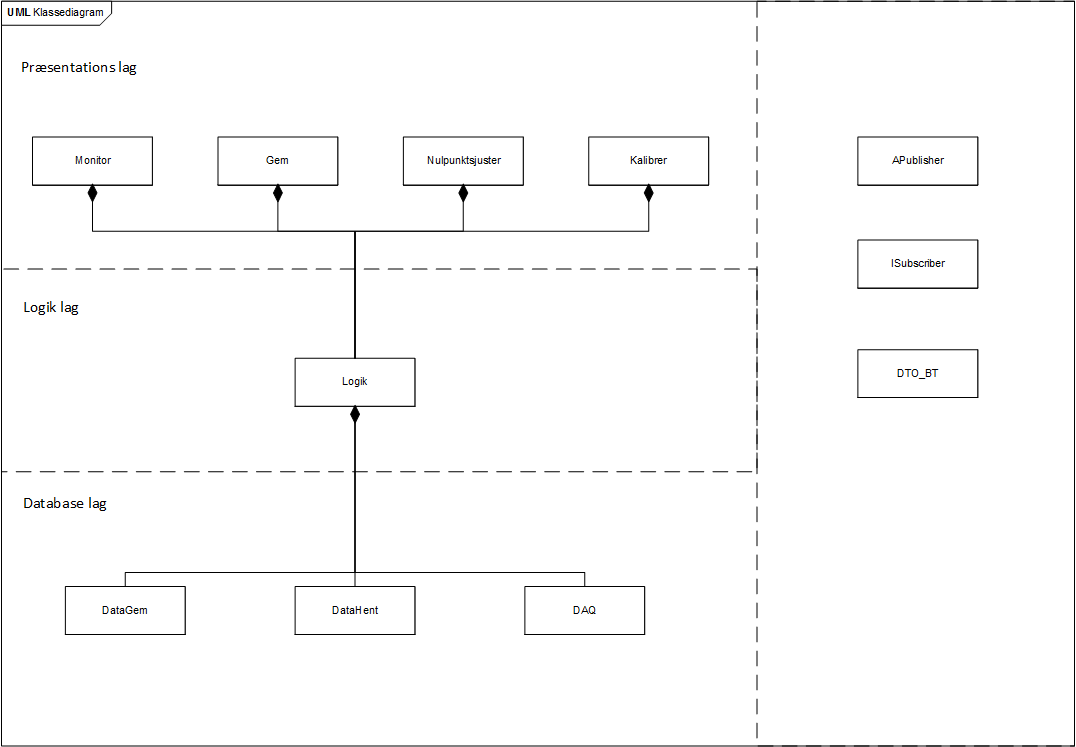
\includegraphics[width=1\textwidth]{Figurer/3lagsmodel_software}
	\caption{UML kompositions klassediagram}
\end{figure}

For at danne et overblik over de forskellige klasser og deres metoder, er der udarbejdet et UML klassediagram. Klassediagrammet beskriver ligeledes relationerne mellem klasserne ved komposition, arv og interface, se Figur 4.2. 

\begin{figure}[H]
	\centering
	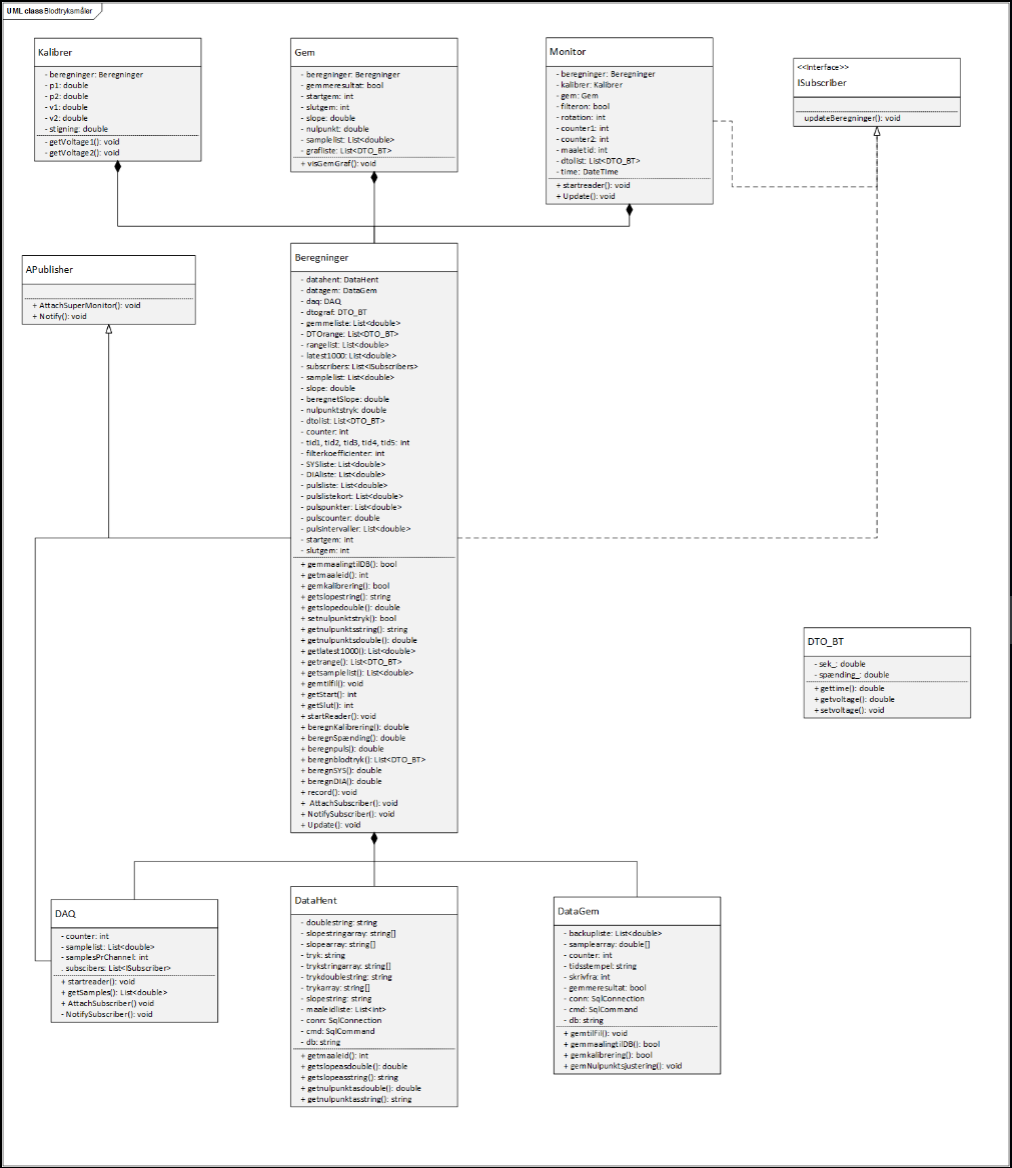
\includegraphics[width=1\textwidth]{Figurer/classdiagram}
	\caption{Klassediagram}
\end{figure}

\subsection{Datalag}
Datalaget kommunikerer med DAQ, Database og computerens harddisk. 

\subsubsection{DAQ}
Klassen DAQ består hovedsageligt af software fra National Instruments, der kan udveksle data med den fysiske DAQ 6009. Denne kan betragtes som af typen ”black box”. Dette betyder, at udvikleren ikke har et begreb om den interne mekanisme i klassen, men udelukkende ser på outputtet. Som udgangspunkt er funktionen af klassen at levere data omkring de målinger, der foretages i den fysiske DAQ.\\
De styrbare parametre i denne klasse er blandt andet samplingfrekvens og måleområde. 

\subsubsection{Datahent}
Klassen henter data fra en Database og lokale tekstfiler. Fra Databasen indhentes data om tidligere målingers nummerering således at de målinger, der skal gemmes i fremtiden, kan blive nummereret korrekt.\\
De lokale tekstfiler indeholder data omkring tidligere kalibreringer og nulpunktsjusteringer.

\subsubsection{DataGem}
Klassen gemmer data på Database og lokale tekstfiler.

\subsection{Logiklag}

\subsubsection{Beregninger}
Beregninger er hovedsageligt et lag, hvor logiske beregninger foretages.\\
Herunder beregnes for eksempel systolisk og diastolisk blodtryk samt puls. Beregninger i forbindelse med kalibrering og nulpunktsjustering foregår ligeledes her. Ydermere skaber logiklaget forbindelse mellem datalaget og præsentationslaget, hvilket tillader, at metoder fra datalaget kan anvendes fra præsentationslaget.

\subsection{Præsentationslag}

\subsubsection{Monitor}
Monitorlaget er Forskerens generelle visuelle interaktionslag med systemet. Heri observeres udskrevne blodtrykssignaler over 4-sekunders intervaller. Værdierne puls, systolisk og diastolisk blodtryk udskrives ligeledes her. Designet er inspireret fra i forvejen eksisterende blodtryksmonitoreringssystemer. \\
Der er mulighed for at vælge en optagelseslængde for målingen, samt starte og stoppe den via en ”Rec”\--knap/"Stop"\--knap. Herefter kan Gem-vinduet åbnes, hvor den optagede sekvens kan gemmes. Derudover er der en knap til udførelse af nulpunktsjustering. Den kørende måling kan vises med eller uden et filter ved at ændre på de to radiobuttons, "On"\-/"Off". Y- og X-akse kan påsættes med to radiobuttons, "On"\-/"Off". Se Figur 4.3.
\begin{figure}[H]
	\centering
	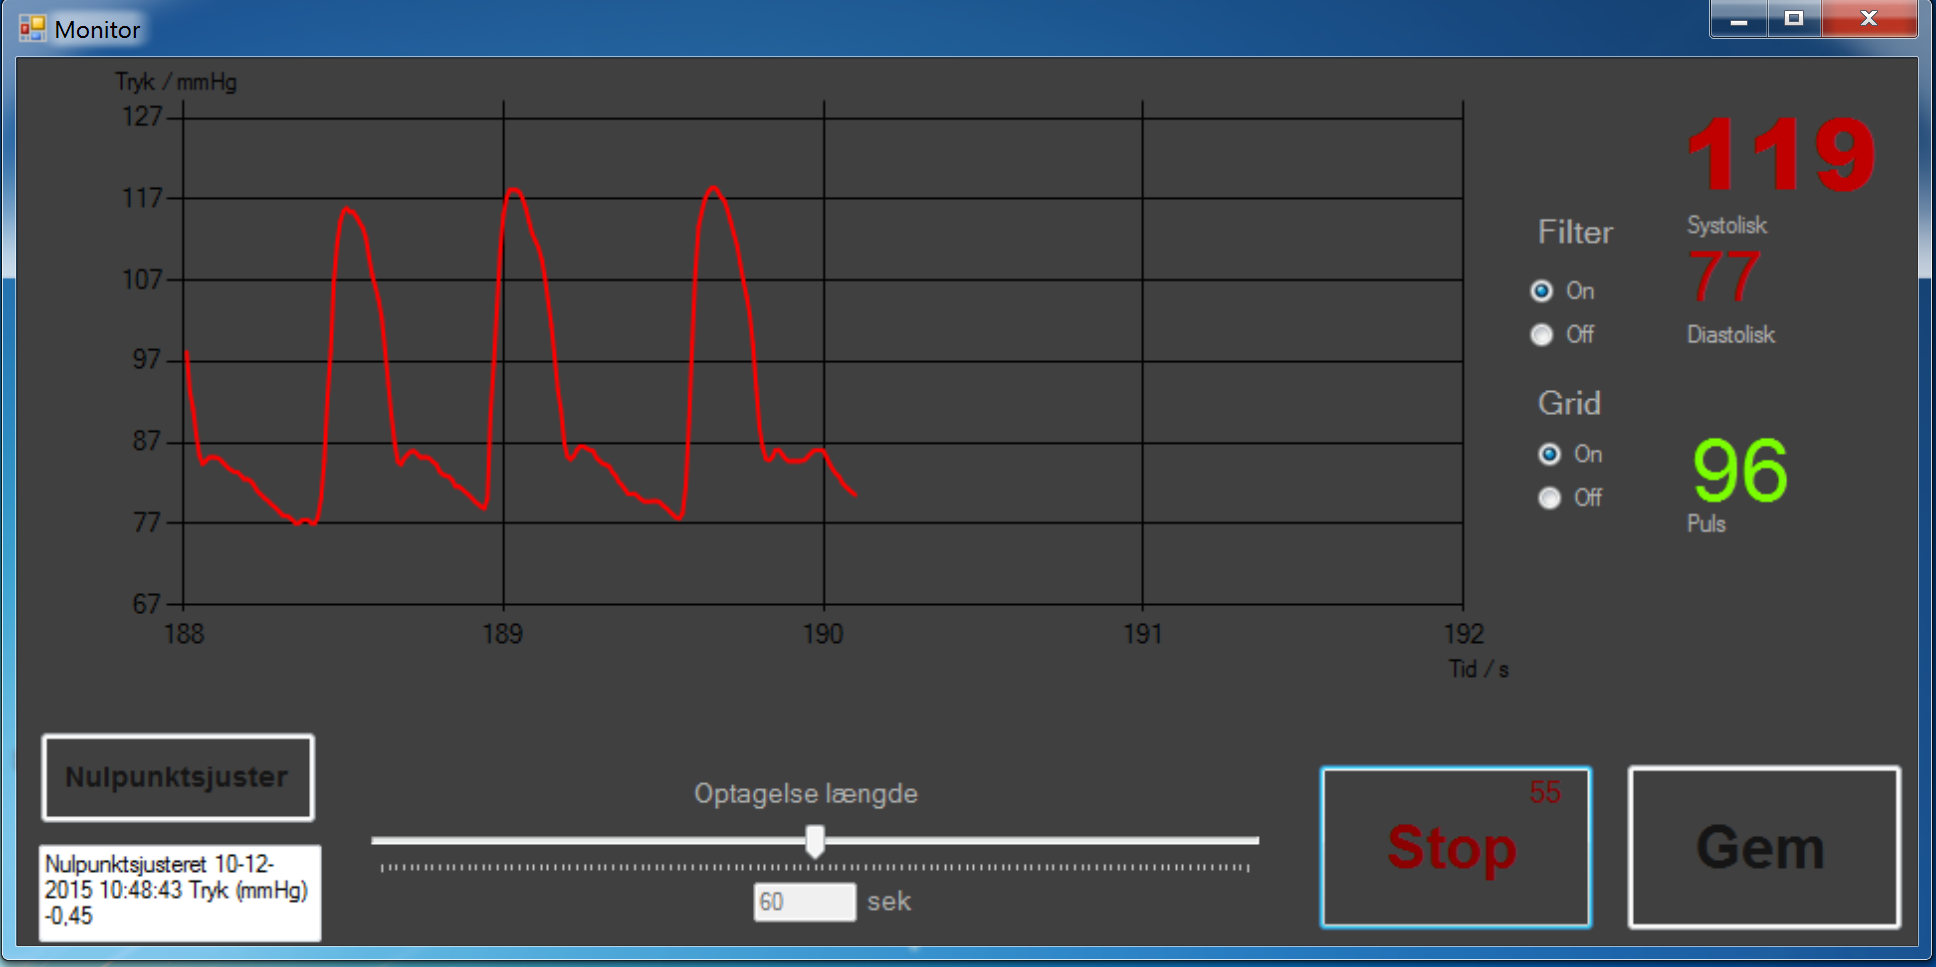
\includegraphics[width=1\textwidth]{Figurer/Monitor_vindue_Recording}
	\caption{Monitor med igangsat måling}
\end{figure}

\subsubsection{Gem}
Vinduet udskriver den optagede sekvens i et vindue, der visuelt ligner Monitor-vinduet. Der er to tekstbokse, hvor en kommentar og et navn for den ansvarlige af målingen, kan indtastes. Se Figur 4.4.
\begin{figure}[H]
	\centering
	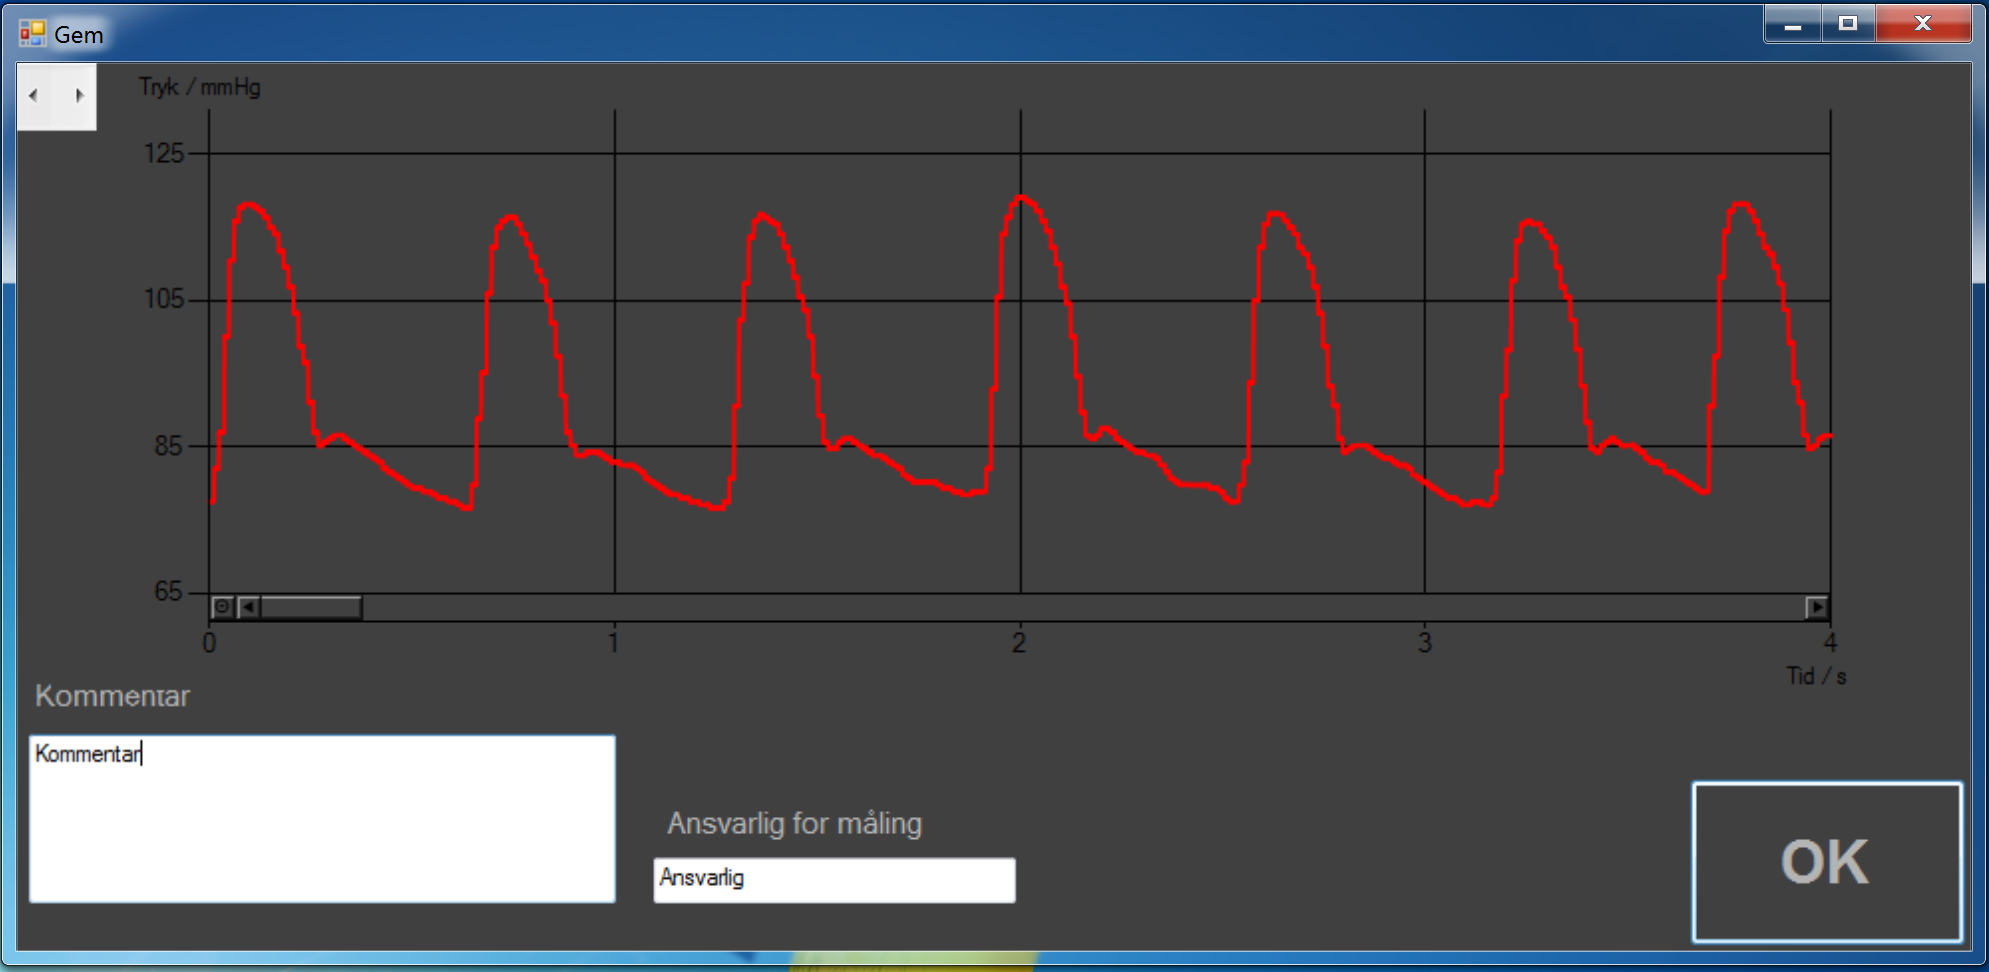
\includegraphics[width=1\textwidth]{Figurer/Gem}
	\caption{Gem-vindue med 10 sekunders måling}
\end{figure}

\subsubsection{Kalibrér}
Vinduet indeholder to tekstbokse til indtastning af tryk samt tekstbokse til dertilhørende spænding. Spændingerne kan måles automatisk ved tryk på ”Mål”\--knapperne.
Kalibreringskonstanten kan udregnes med knappen ”Beregn” og gemmes samt anvendes ved at trykke på ”OK”\--knappen.

\subsection{Datamodellaget}
Datamodellaget muliggør indirekte dataoverførsel mellem lag, der umiddelbart ikke har relation, der tillader dette.

\subsubsection{DTO}
DTO er et namespace, som indeholder data transfer object (DTO). Alle de andre lag har adgang til dette lag og kan oprette instanser af klassen DTO.\\
Denne klasse har attributterne tid og spænding. Formålet med denne klasse er at overføre sampleværdier fra DAQ til et format, der har en korrekt tidsværdi, samt et tryk korrigeret for nulpunktstryk og kalibrering.
\begin{figure}[H]
	\centering
	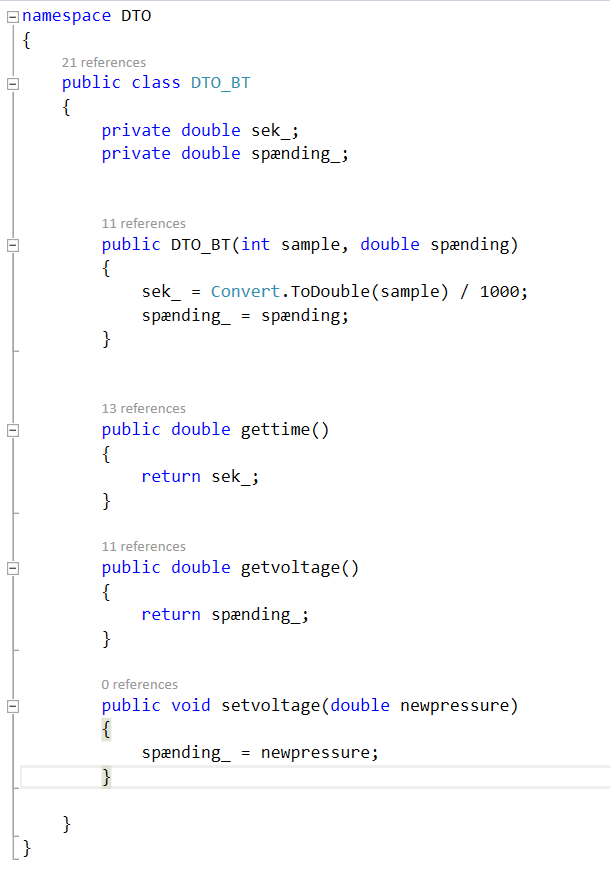
\includegraphics[width=0.5\textwidth]{Figurer/DTO_kode}
	\caption{DTO klassen med metoder}
\end{figure}

\subsubsection{Publisher/subscriber pattern}
Datastrømmen fra DAQ klassen er styrende for alle de andre klasser, blandt andet udskrivning af blodtrykket i Monitor-vinduet. Den fysiske DAQ måler med 1000 Hz og returnerer data til DAQ klassen med 50 ms intervaller. Dette måleinterval indeholder 50 sampleværdier. Disse data sendes videre til Beregningerklassen, og fra Beregningerklassen til Monitorklassen ved hjælp af publisher/subscriber mønstret. Når data befinder sig i Monitorklassen kan der laves logiske beregninger og manipulation på data i Beregningerklassen.\\
Forholdet mellem klasserne er således, at DAQklassen og Beregningerklassen har et publisher/subscriber forhold, og  Beregninger- og Monitorklassen har et publisher/subscriber forhold. \\
Hierakiet fremgår af Figur 4.6, Figur 4.7, og Figur 4.8.
\begin{figure}[H]
	\centering
	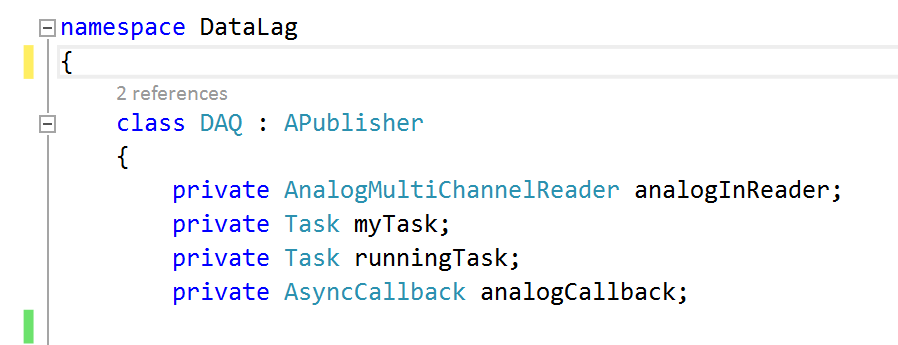
\includegraphics[width=0.5\textwidth]{Figurer/DAQ_pub}
	\caption{DAQ klassens arvehieraki}
\end{figure}

\begin{figure}[H]
	\centering
	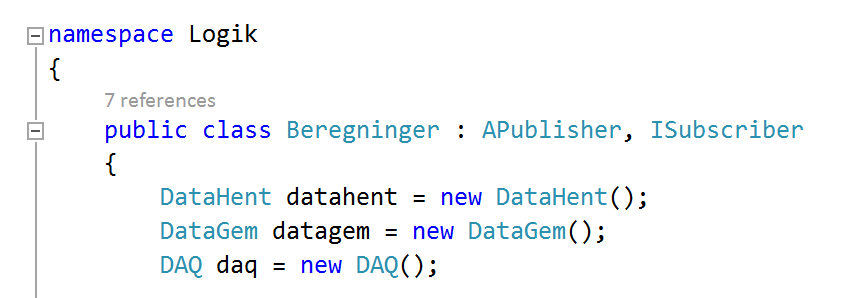
\includegraphics[width=0.5\textwidth]{Figurer/Beregninger_subpub}
	\caption{Beregninger klassens arvehieraki}
\end{figure}

\begin{figure}[H]
	\centering
	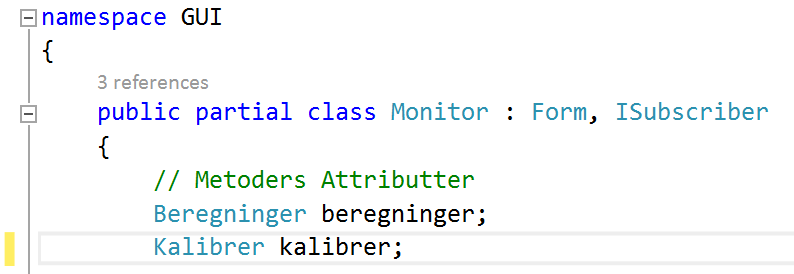
\includegraphics[width=0.5\textwidth]{Figurer/Monitor_sub}
	\caption{Monitor klassens arvehieraki}
\end{figure}


\subsection{Metodebeskrivelser}

De seks Use Cases er beskrevet ved hjælp af sekvensdiagrammer med korte beskrivelser herunder. Dette gøres for at se, hvilke klasser og metoder i softwaren der bruges i de forskellige Use Cases.\\
Sekvensdiagrammerne overskueliggør klassernes involvering i de forskellige Use Cases og beskriver kommunikationen herimellem.\\
Aktivitetsdiagrammer beskriver udførelsen af enkelte metoder step-by-step. Dette giver et fuldkomment indblik i metodens workflow.


\subsubsection{Use Case 1: Kalibrer}
Forsker trykker på knappen "Beregn"\- og anmoder Kalibreringsklassen om metoden 'beregn' i Beregningerklassen. Den udregnede kalibreringskonstant returneres.\\
Forsker trykker på knappen "OK"\- og metoden 'gemkalibrering' afvikles i Beregningerklassen. Herfra afvikles metoden 'gemkalibrering' i DataGemklassen. DataGem returnerer en bool, der beskriver om gemningen var succesfuld.
\begin{figure}[H]
	\centering
	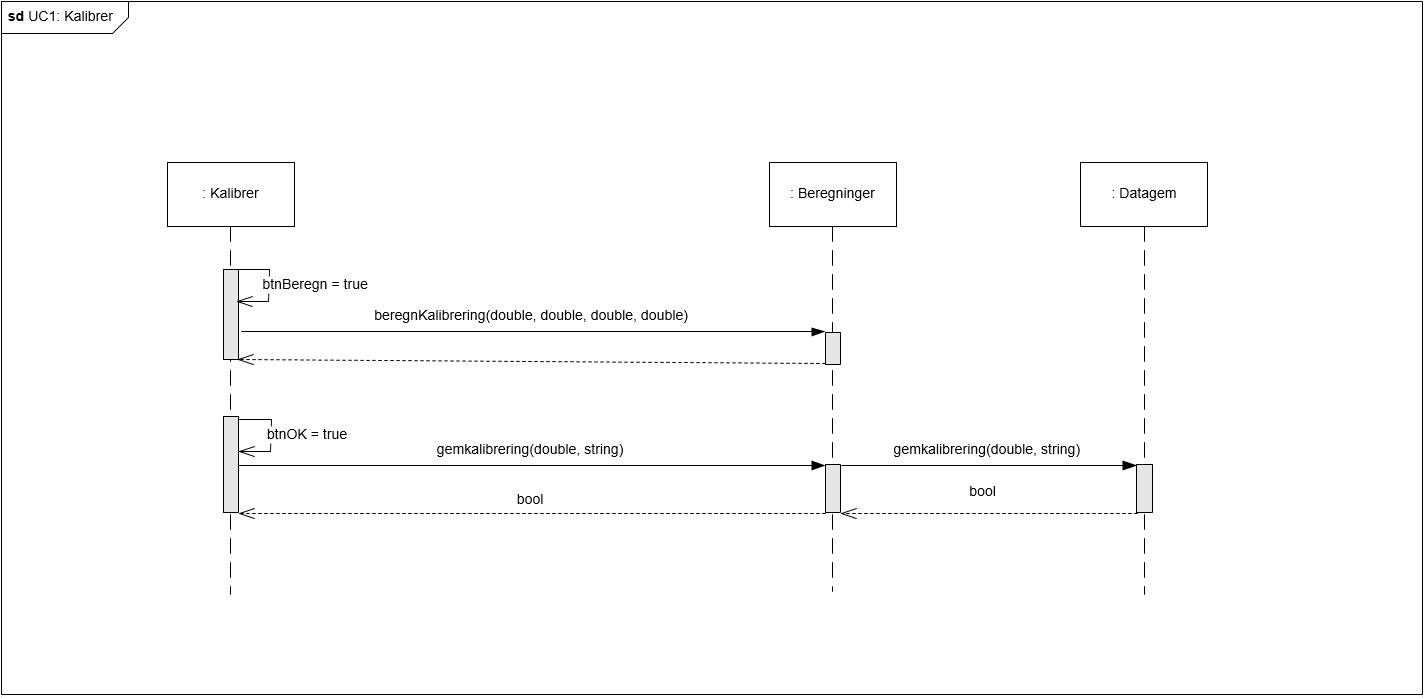
\includegraphics[width=1\textwidth]{Figurer/UC1_SD_SW}
	\caption{Sekvensdiagram for Use Case 1}
\end{figure}

\subsubsection{Use Case 2: Vis måling med filter}
Når Monitor-vinduet åbnes ved opstart af program afvikles metoden 'startreader' i DAQ klassen. Ved hjælp af publisher/subscriber metoden, 'NotifySubscriber', returneres rådata til Beregninger og videre til Monitor.\\
Rådata sendes til Beregninger og omregnes til tid og blodtryk ved hjælp af DTO klassen.
'BeregnSYS', 'beregnDIA' og 'beregnPuls' returnerer ligeledes double værdier med systolisk og diastolisk blodtryk samt puls. 
\begin{figure}[H]
	\centering
	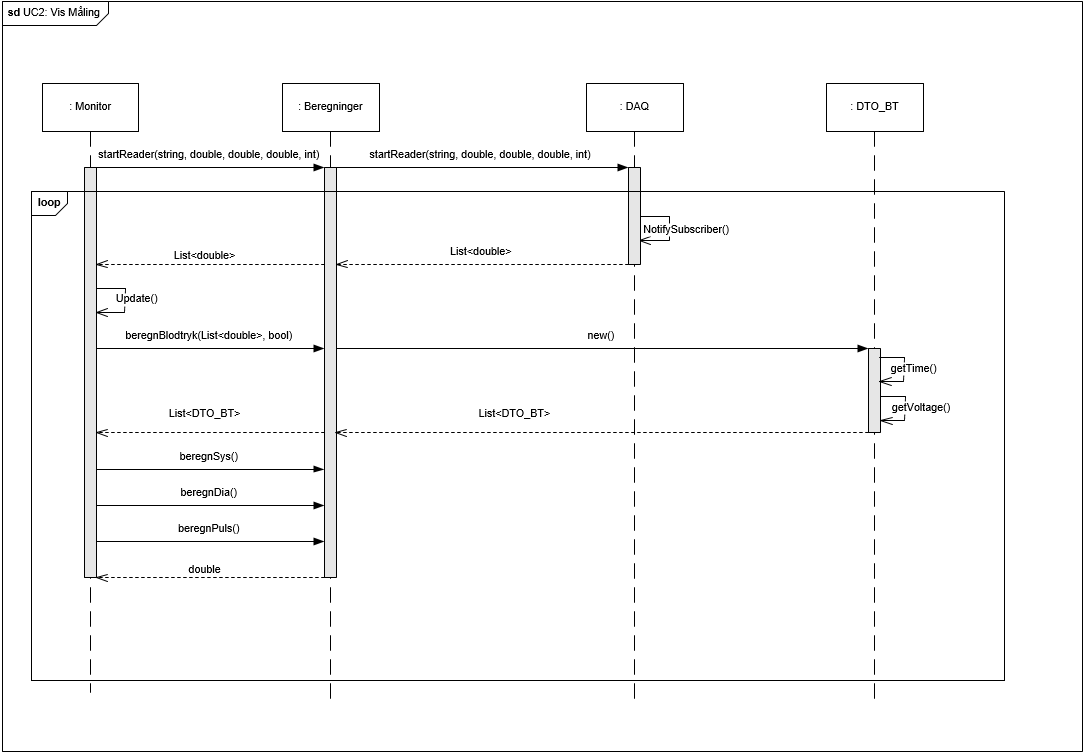
\includegraphics[width=1\textwidth]{Figurer/UC2_SD_SW}
	\caption{Sekvensdiagram for Use Case 2}
\end{figure}

Metoden, der beregner puls, har to logiske grene til udregning af pulsen. Den første gren til venstre i Figur 4.11 beregner pulsen, når der er mellem 3000 og 10000 samples til rådighed - altså når den fysiske DAQ har målt mellem 3 og 10 sekunder.\\
Metodikken består i at lokalisere toppunkter i signalet for at udregne det gennemsnitlige interval herimellem. Herudfra kan pulsen estimeres. \\
En for-løkke bruges til at evaluere alle sampleværdier i forhold til de førliggende og efterfølgende samples. Hvis værdien på den pågældende sample har større værdi end den førliggende og efterfølgende, gemmes tidspunktet for dette sample i en liste.\\ 
For at sikre at toppunktet ikke er et mindre toppunkt, fra eksempelvis støj eller højfrekvent signalindhold, evalueres der kun for hver 50. værdi, og tidspunktet gemmes kun, hvis værdien ligger 0,1 V over gennemsnittet af alle sampleværdier der evalueres. Ud fra gennemsnitsintervallet mellem toppunkterne beregnes pulsen.
\\
\\
Den anden logiske gren regner pulsen, når der er over 10000 samples til rådighed - altså efter den fysiske DAQ har målt i over 10 sekunder.\\ 
Metodikken er den samme som ovenfor, men i stedet for at gemme et tidspunkt for toppunktet, tælles en counter op. Når antallet af toppunkter for 10 sekunder er fundet, kan pulsen beregnes.

\begin{figure}[H]
	\centering
	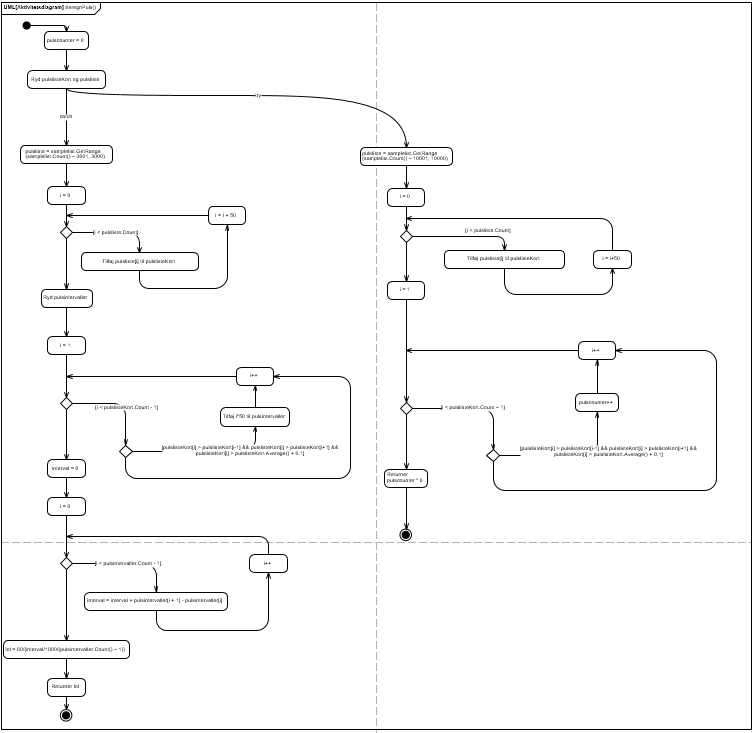
\includegraphics[width=1\textwidth]{Figurer/aktivitetsdiagram_beregnPuls}
	\caption{Aktivitetsdiagram over beregnpuls}
\end{figure}


\subsubsection{Use Case 3: Nulpunktjuster}
'GetNulpunktsstring' returnerer en string, der indeholder data om seneste nulpunktsjustering. Denne udskrives på Monitor.\\
Forsker trykker på knappen 'Nulpunktsjuster', og Beregninger udfører en nulpunktsjustering, gemmer data i DataGem og returnerer en ny string der beskriver den seneste nulpunktsjustering.

\begin{figure}[H]
	\centering
	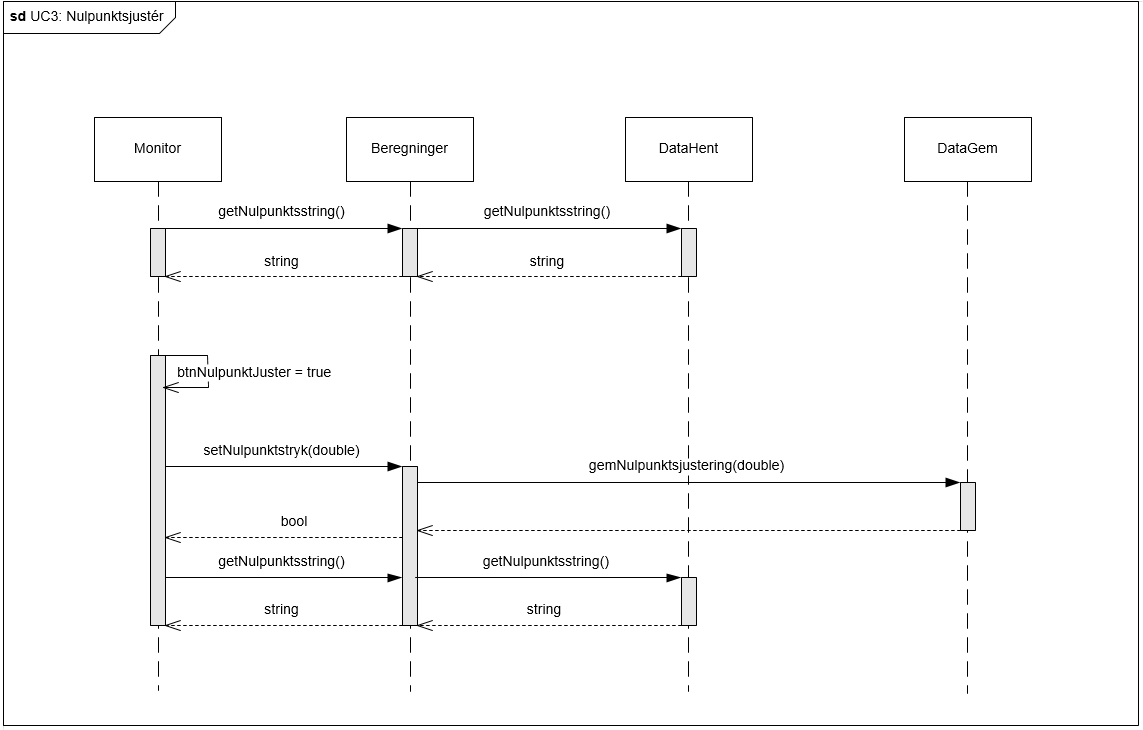
\includegraphics[width=1\textwidth]{Figurer/UC3_SD_SW}
	\caption{Sekvensdiagram for Use Case 3}
\end{figure}

\subsubsection{Use Case 4: Deaktiver filter}
Forsker sætter radiobutton for filter til "Off".
Boolen "filteron" sættes til 'false', og sendes med metoden, der udregner blodtryk 'beregnBlodtryk', i Beregningerklassen. Den returnerede liste af DTO'er, som udskrives i Monitor, er ufiltrerede.

\begin{figure}[H]
	\centering
	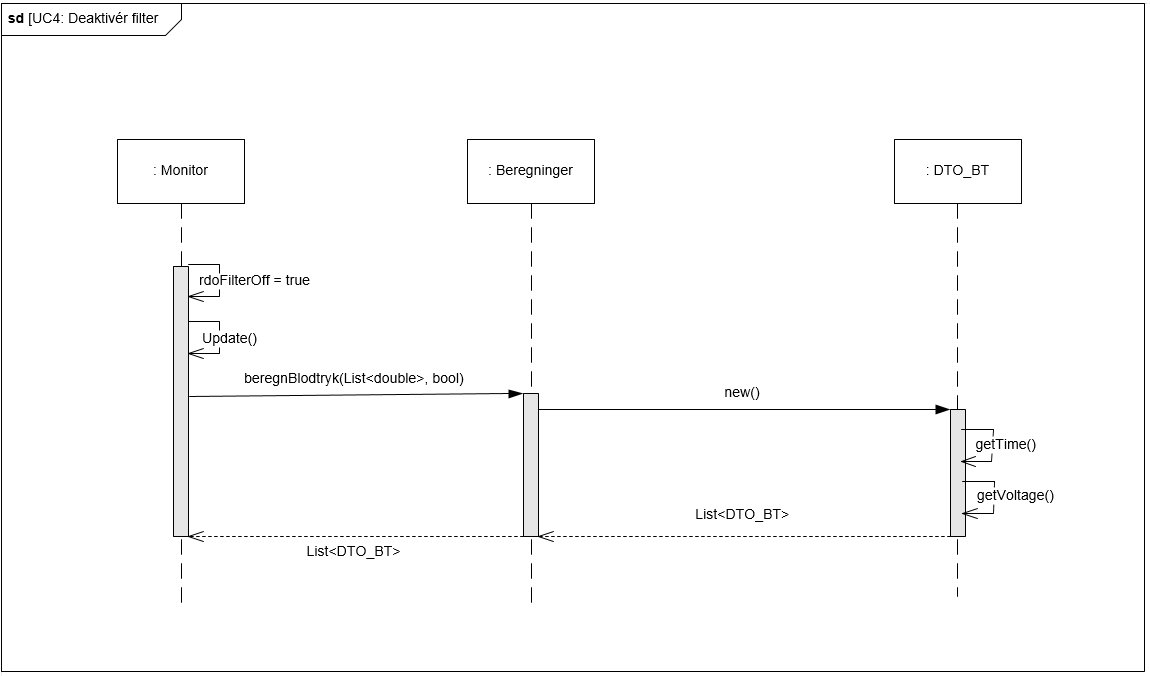
\includegraphics[width=1\textwidth]{Figurer/UC4_SD_SW}
	\caption{Sekvensdiagram for Use Case 4}
\end{figure}

\subsubsection{Use Case 5: Aktiver filter}
Filteret er bygget op som et FIR-filter med 10 filterkoefficienter. Hvert udskrevet punkt på grafen er en gennemsnitsværdi af de foregående 10 værdier.
Forsker sætter radiobutton for filter til "On".
Boolen "filteron" sættes til 'true', og sendes med metoden, der udregner blodtryk 'beregnBlodtryk', i Beregningerklassen. Den returnerede liste af DTO'er, som udskrives i Monitor, er filtrerede.

\begin{figure}[H]
	\centering
	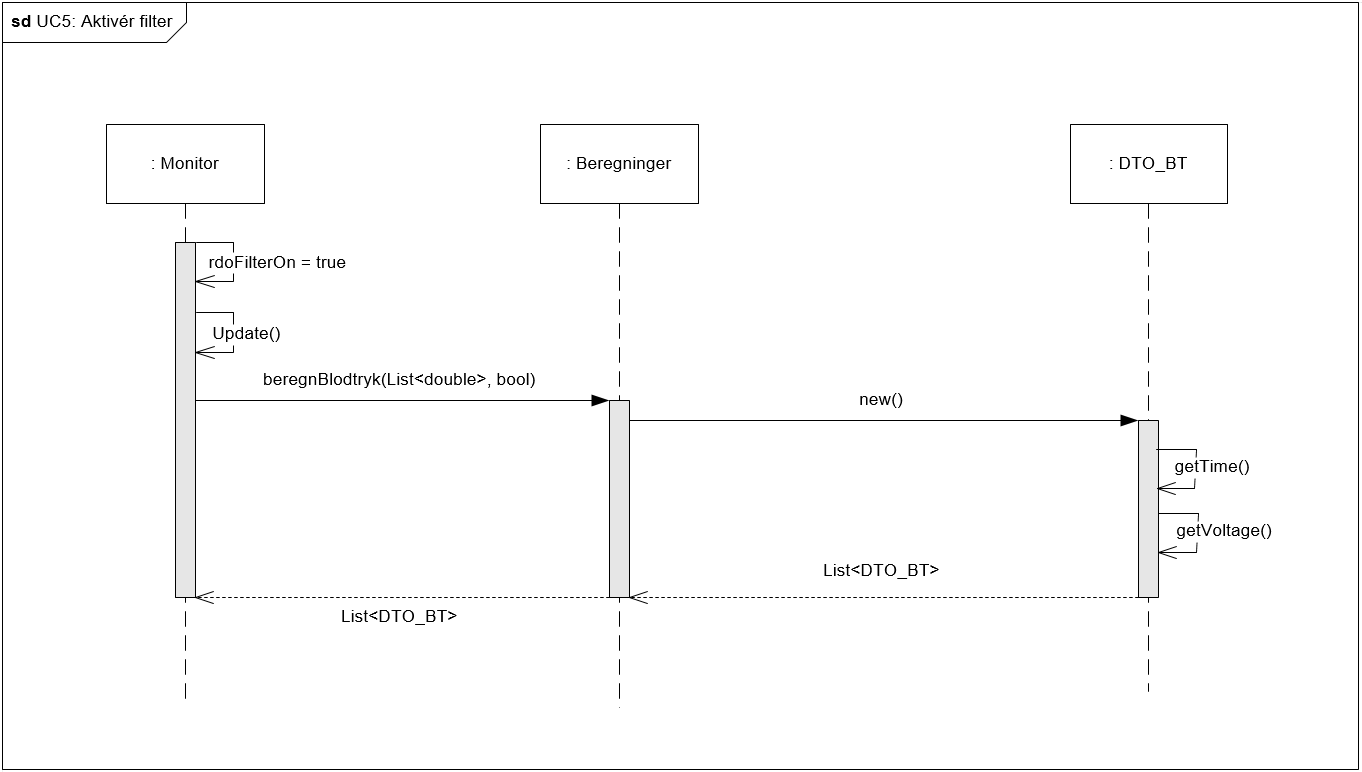
\includegraphics[width=1\textwidth]{Figurer/UC5_SD_SW}
	\caption{Sekvensdiagram for Use Case 5}
\end{figure}

\subsubsection{Use Case 6: Gem måling}
Forsker vælger en optagelseslængde og trykker på "Rec". Metoden record() køres i Beregningerklassen og der sættes en startværdi for målingen.
Når tiden udløber, køres record() i Beregningerklassen igen og en slutværdi for målingen sættes.
Forsker trykker på "Gem"\--knappen i Monitor-vinduet og et Gem-vindue instantieres med data fra den optagede måling. Disse hentes via metoder i logiklaget.\\
Det optagede signal vises i Gem-vinduet. Dette gøres ved hjælp en liste af DTO'er, der oprettes.\\

Forsker trykker på "OK"\--knappen
og metoden gemmaalingtilDB() afvikles i DataGem klassen. Det målte signal og metadata gemmes. 

\begin{figure}[H]
	\centering
	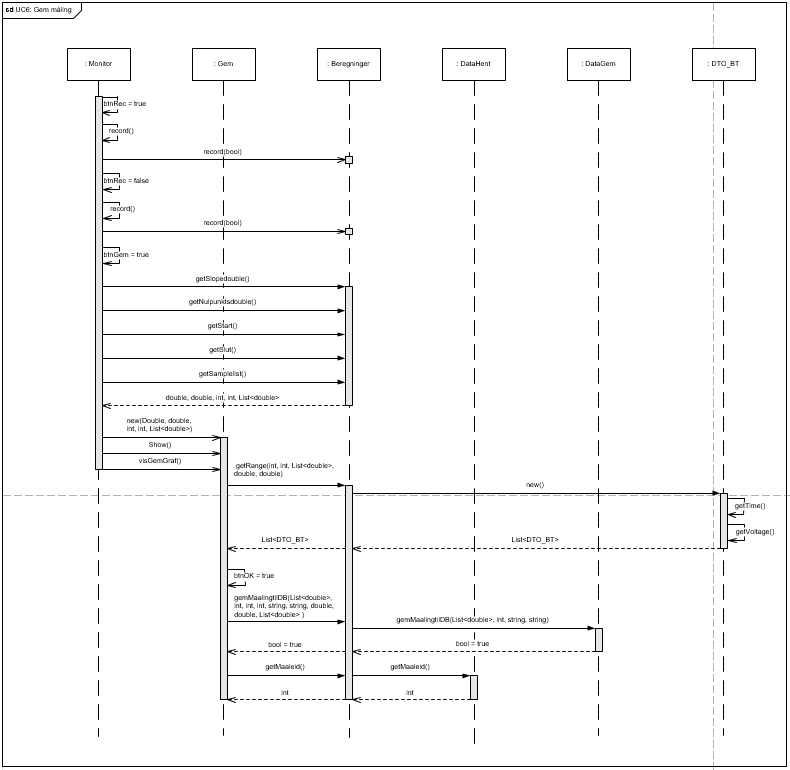
\includegraphics[width=1\textwidth]{Figurer/UC6_SD_SW}
	\caption{Sekvensdiagram for Use Case 6}
\end{figure}

\section{Test}
Til at teste de forskellige metoder i softwaren er der blevet benyttet debugging. Debugging gør det muligt at følge compilerens sekventielle udførelse af programmet. Når der udføres handlinger, og attributværdier sættes, kan dette følges og sættes op mod de forventede resultater. Såfremt der skulle opstå fejl, gør debugging det muligt at fokusere på enkelte metoder og undersøge, hvor fejlen opstår.

\subsection{Use Case 1: Kalibrer}

Forsker indtaster målte kalibreringsdata. Kalibreringsdata for seneste kalibrering vises. Se Figur 4.16.

\begin{figure}[H]
	\centering
	\includegraphics[width=1\textwidth]{Figurer/Test_Kalibrer_1}
	\caption{Kalibreringsdata indtastet}
\end{figure}

De målte værdier beregnes. Se Figur 4.17.

\begin{figure}[H]
	\centering
	\includegraphics[width=1\textwidth]{Figurer/Test_Kalibrer_2}
	\caption{Kalibreringskonstant udregnes}
\end{figure}

Kalibreringskonstanten implementeres ved udskrivning på graf. Se Figur 4.18.

\begin{figure}[H]
	\centering
	\includegraphics[width=1\textwidth]{Figurer/Test_Kalibrer_3}
	\caption{Kalibreringsdata anvendes}
\end{figure}
Det kontrolleres, at kalibreringsfilen er opdateret. Se Figur 4.19.
\begin{figure}[H]
	\centering
	\includegraphics[width=1\textwidth]{Figurer/Test_Kalibrer_4}
	\caption{Kalibreringsdata er gemt til fil}
\end{figure}

\subsection{Use Case 2 Vis måling}
Et inputsignal på 1 Hz, 1 V amplitude og 0 V offset bruges til input på den fysiske DAQ. Se Figur 4.20.
\begin{figure}[H]
	\centering
	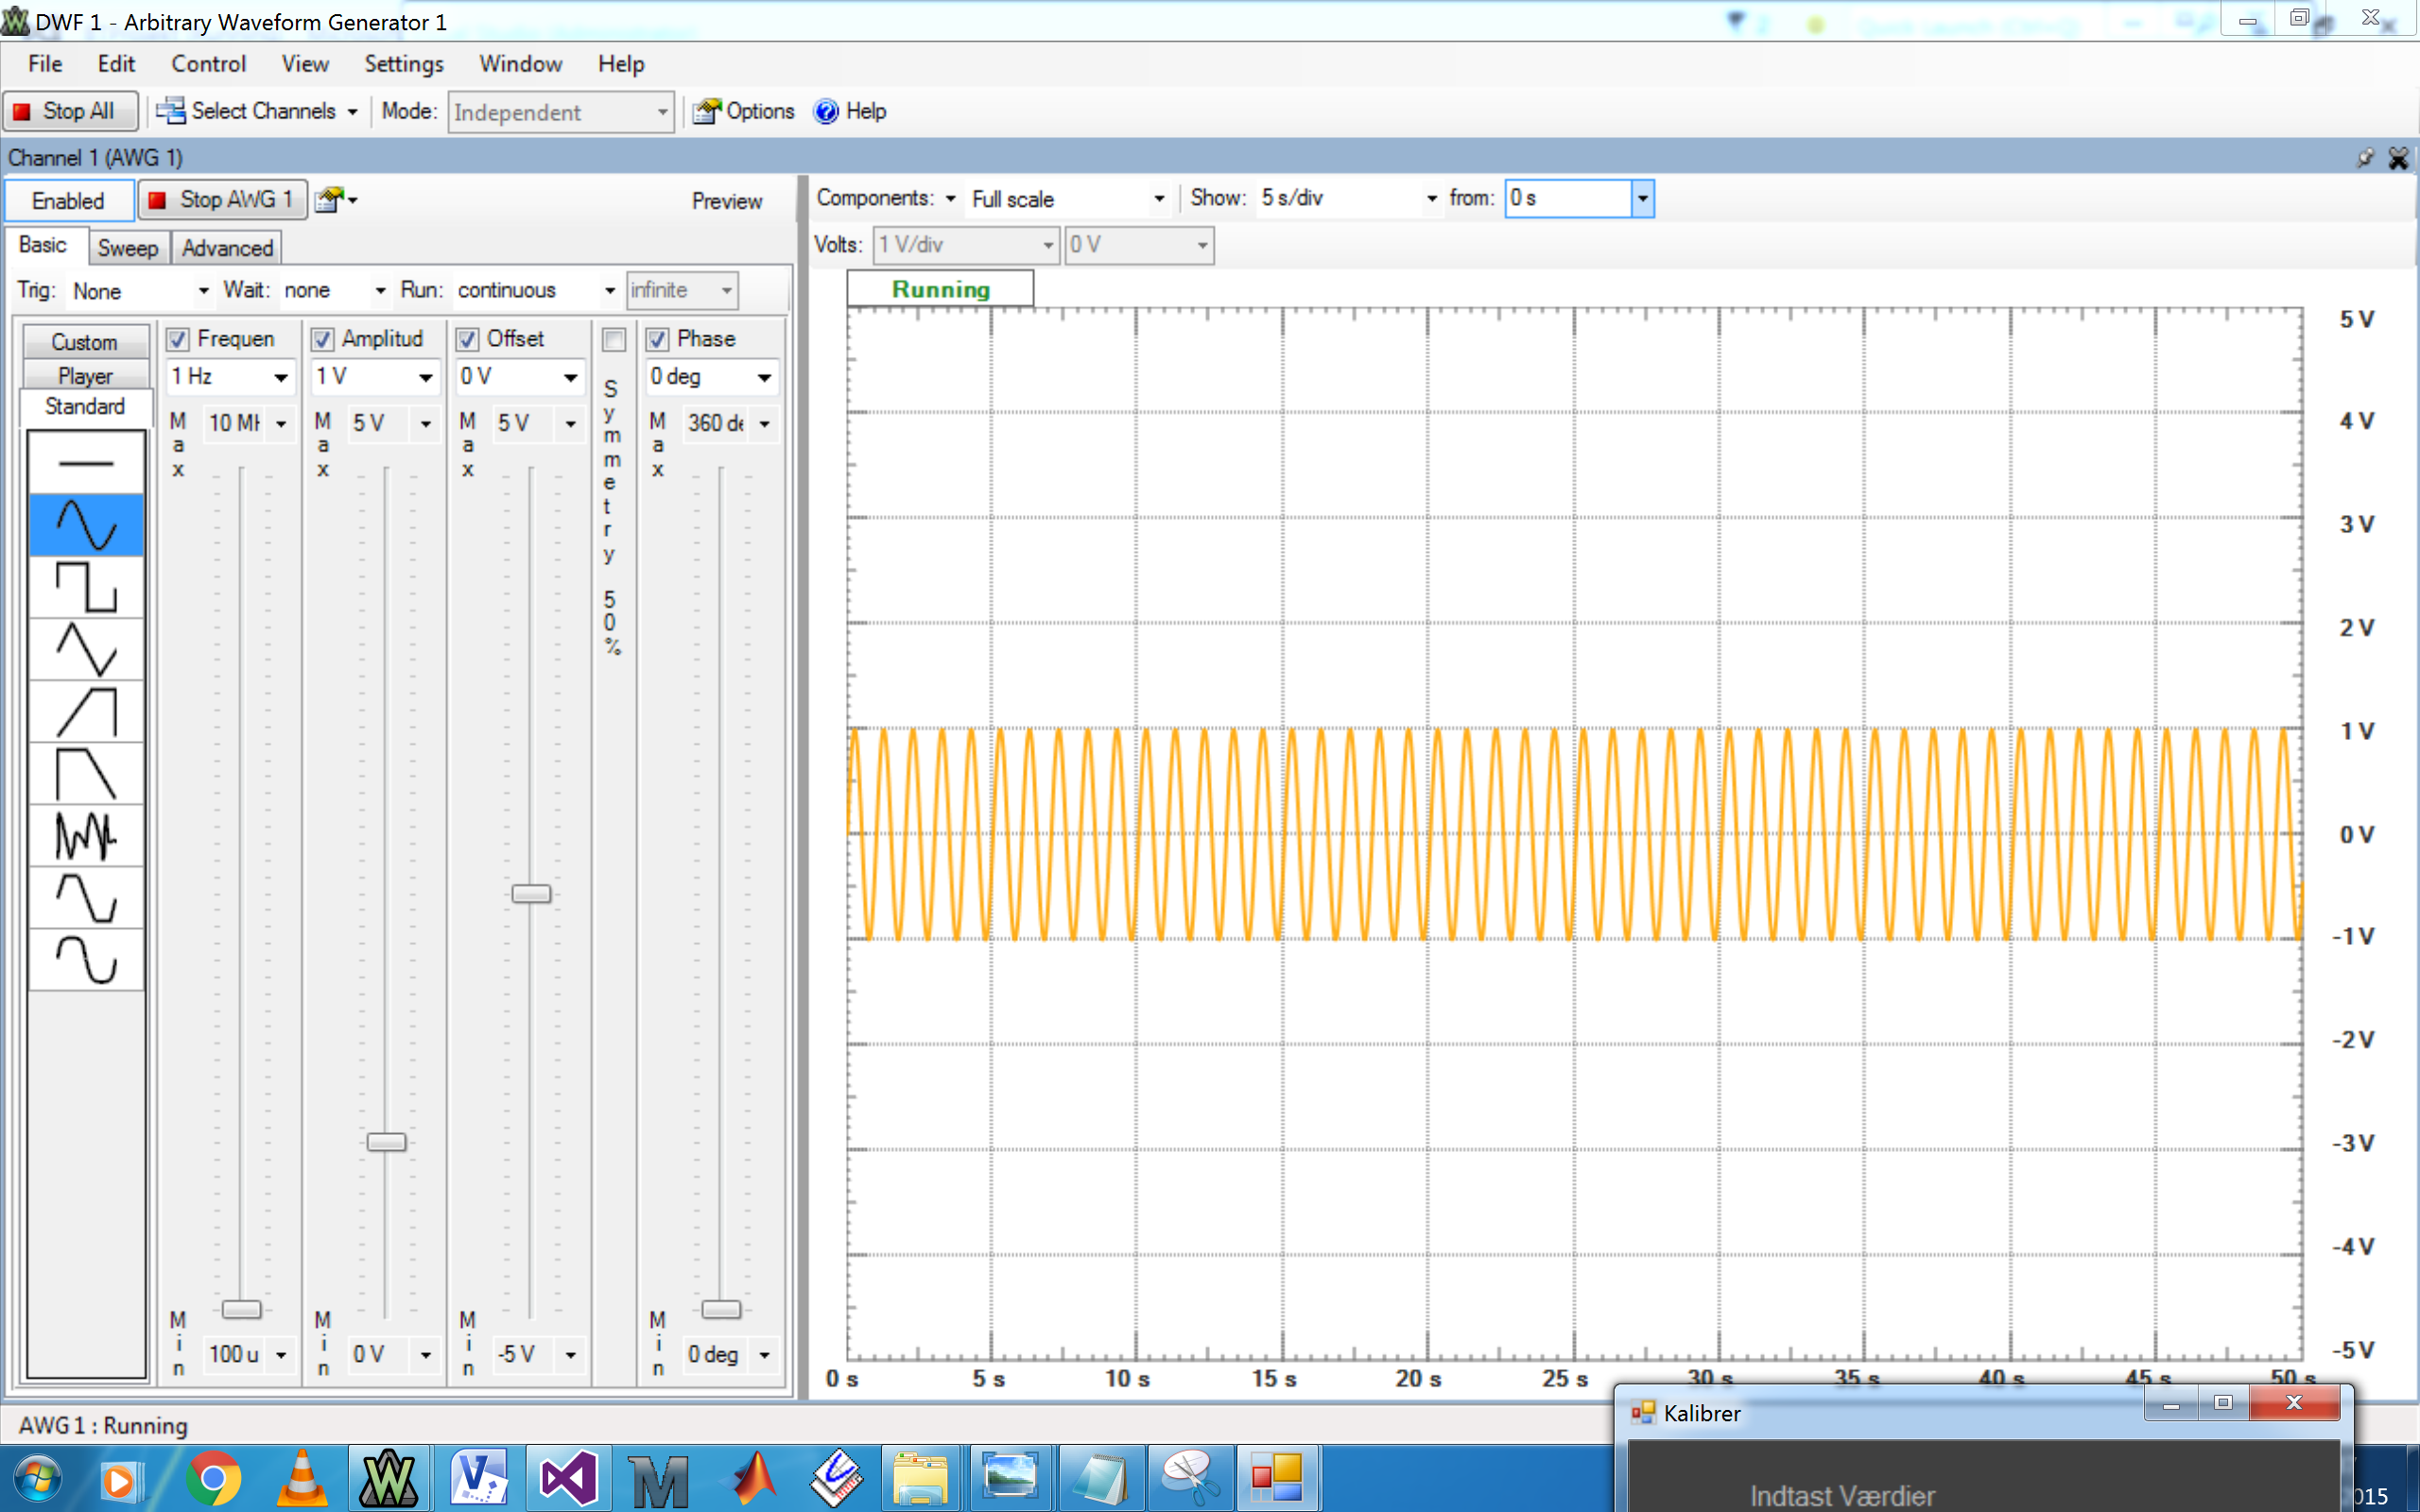
\includegraphics[width=1\textwidth]{Figurer/Test_Vis_1}
	\caption{Inputsignal til DAQ}
\end{figure}

Det ses, at kalibreringskonstanten (mmHg/V) er lig 57,9.
Nulpunktsjusteringsværdien er tæt på 0.
Maksimalværdien på signalet (systole) skal være lig 58 mmHg.
Minimumsværdien på signalet skal være lig -58 mmHg. 
Pulsen skal være lig 60 (1 Hz).  Se Figur 4.21.

Kalibreringskonstanten er lig 57,9. Det udskrevne blodtryk er lig 57,9 mmHg.
\begin{figure}[H]
	\centering
	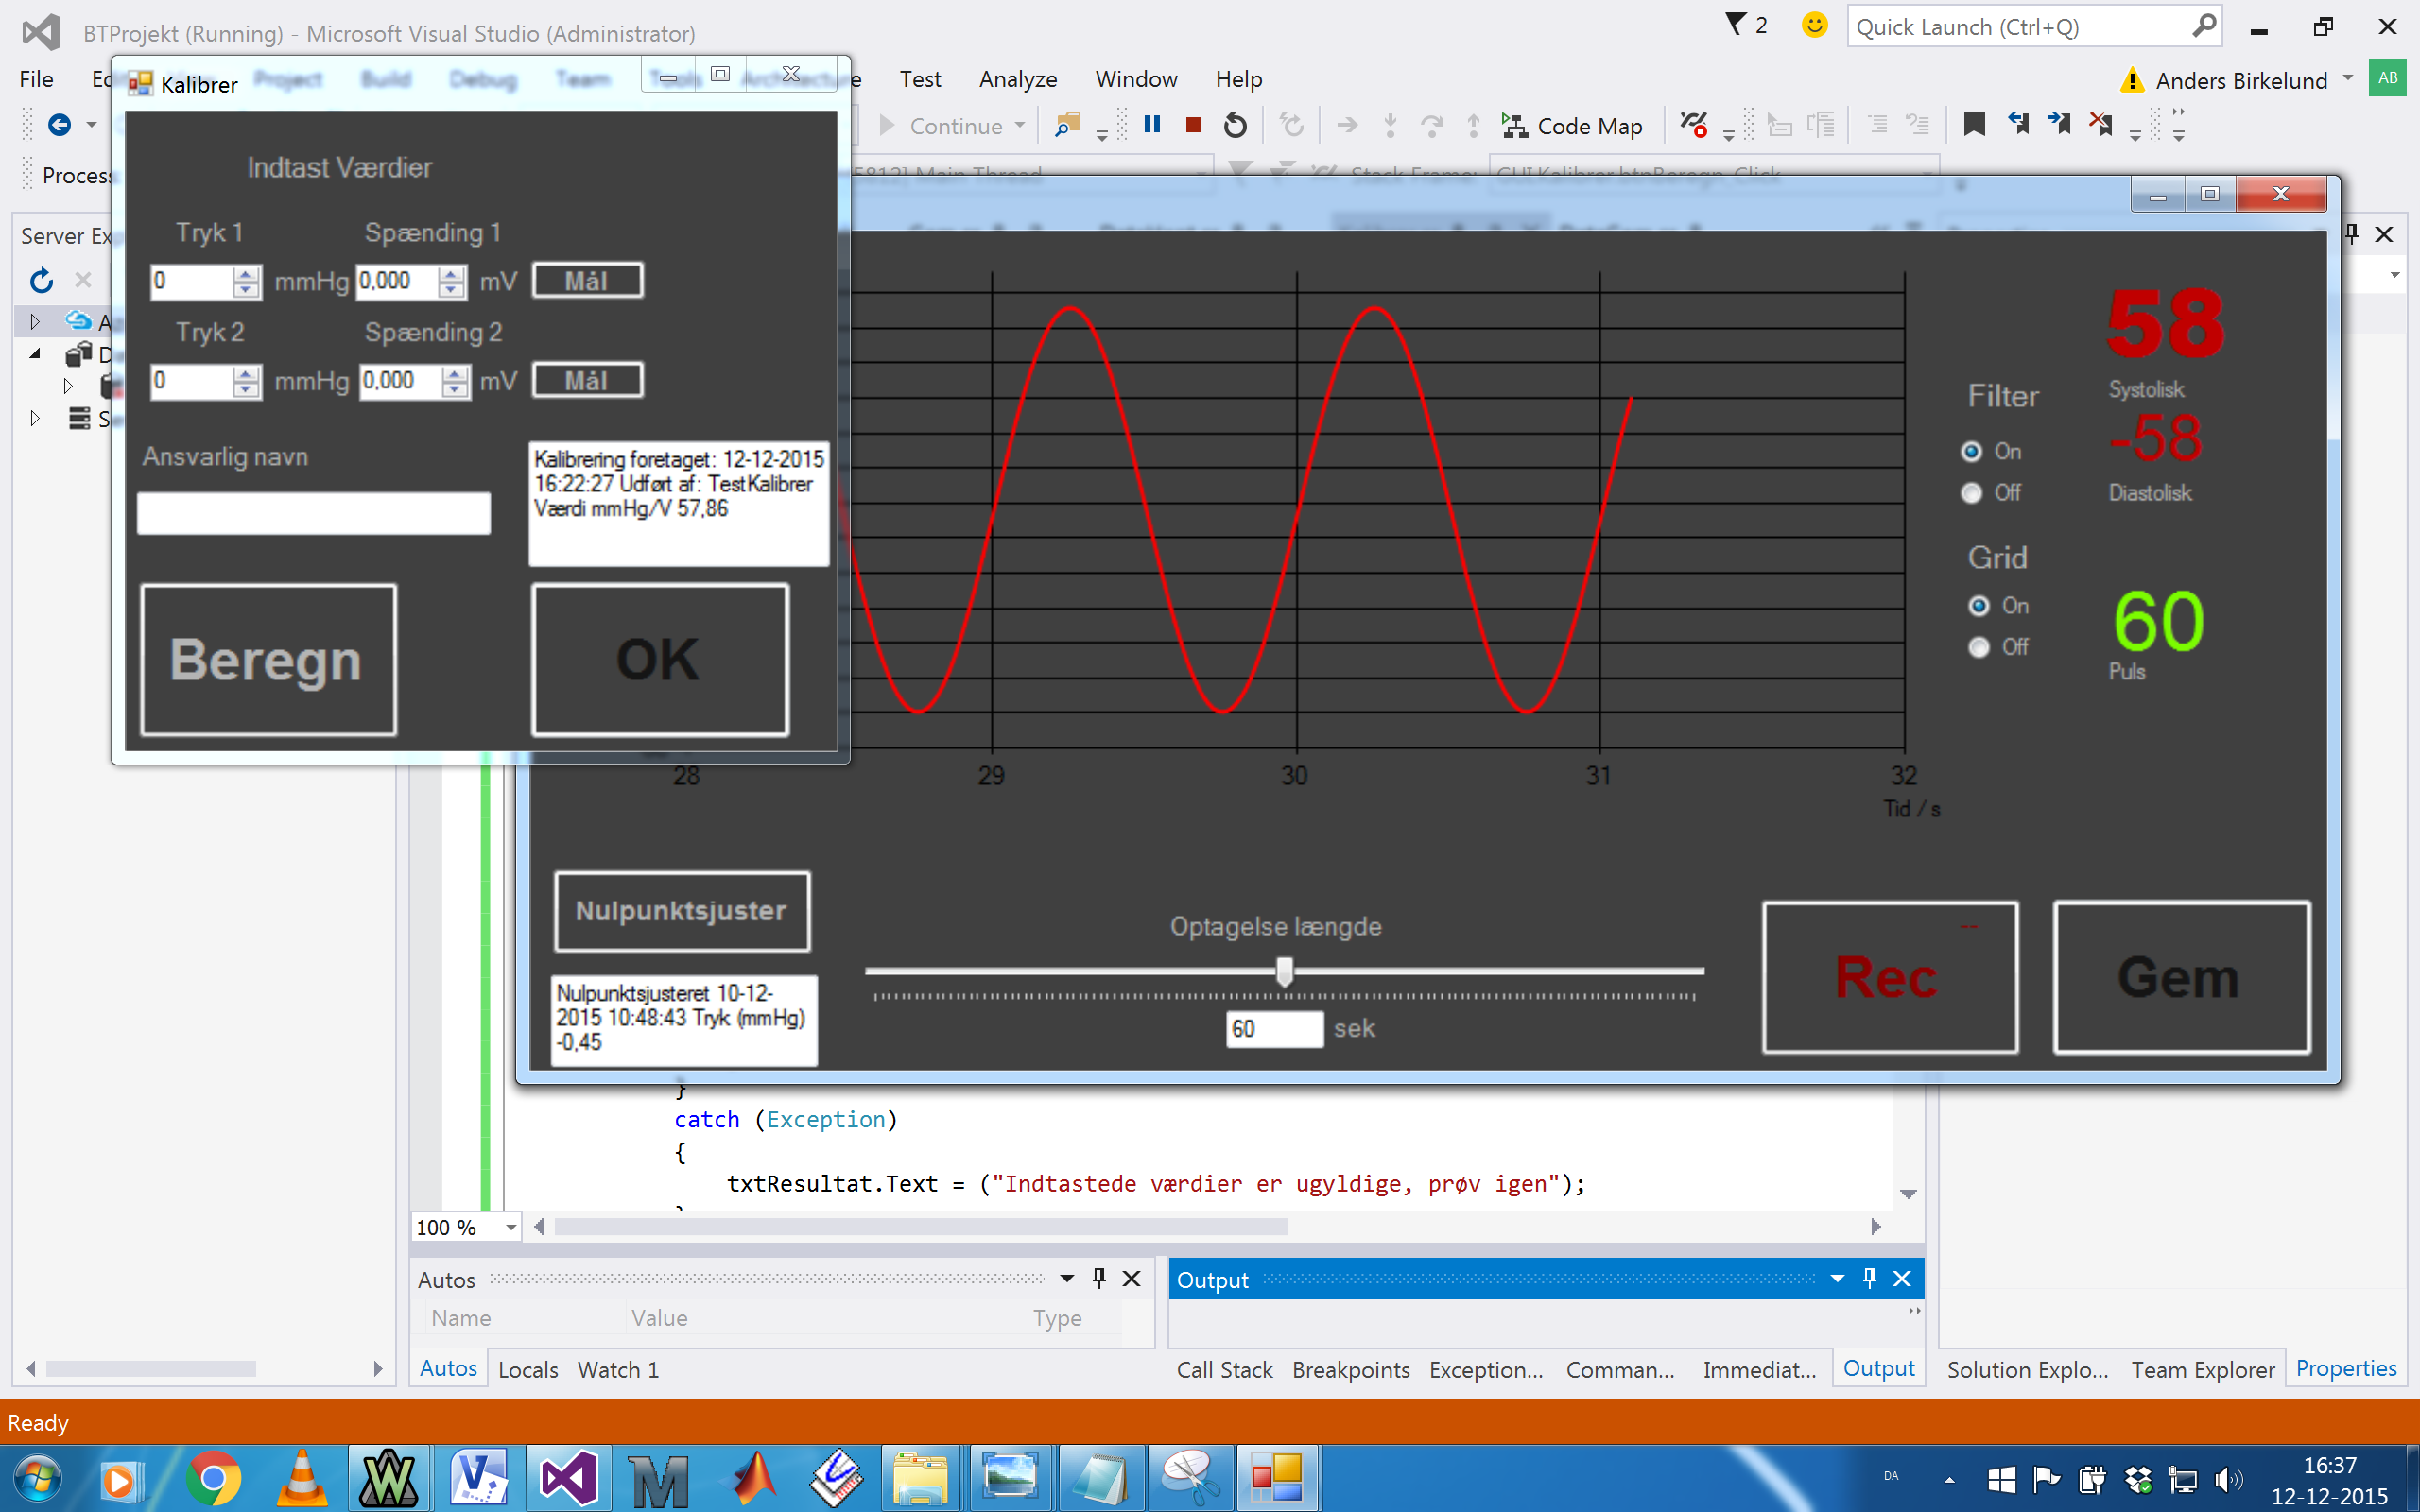
\includegraphics[width=1\textwidth]{Figurer/Test_Vis_2}
	\caption{Output på Monitor-vindue}
\end{figure}

\subsubsection{Puls}
Til at teste pulsmetoden startes en optagelse fra starten af målingen. Målelængden sættes til 10 sekunder. Disse parametre sættes i Monitor-vinduets constructor, så optagelsen starter lige så snart måling startes. Se Figur 4.22.
\begin{figure}[H]
	\centering
	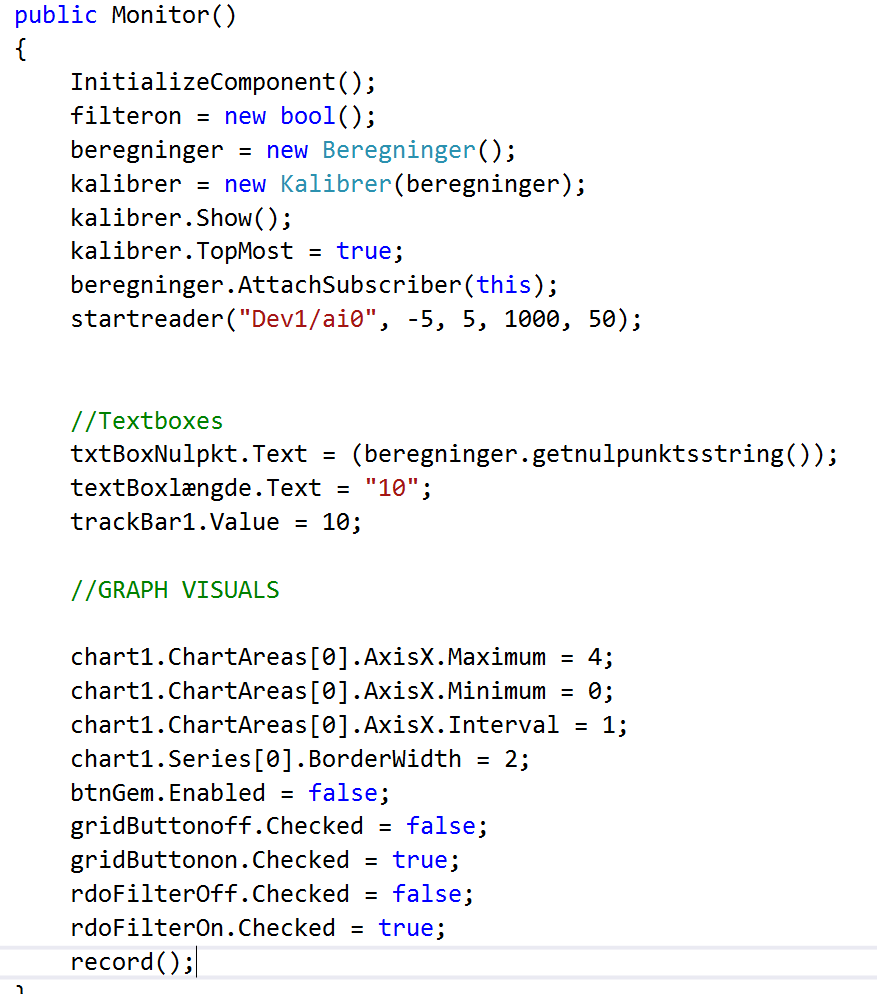
\includegraphics[width=0.5\textwidth]{Figurer/Pulstest_record}
	\caption{Monitor-vinduets default constructor ved puls-test}
\end{figure}
Et break point sættes ved metoden, der returnerer en puls, baseret på 10000 samples. Metoden har talt 15 pulsslag. Se Figur 4.23.
\begin{figure}[H]
	\centering
	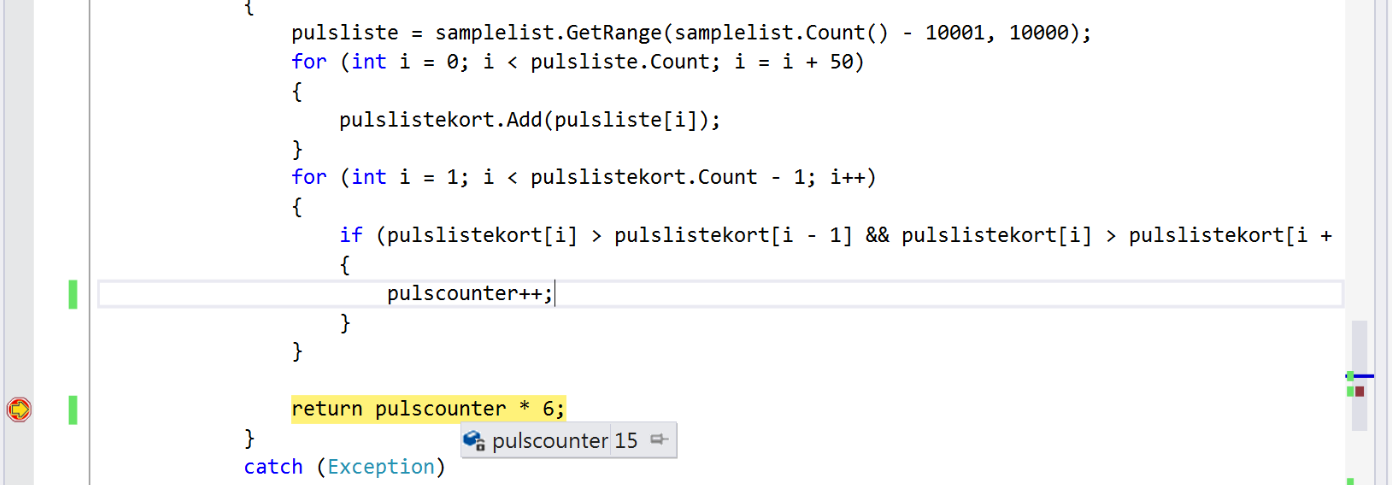
\includegraphics[width=1\textwidth]{Figurer/Pulstest_debug}
	\caption{Puls efter 10 sekunders måling}
\end{figure}
Antallet af pulsslag talt på Gem-vinduet for de 10 sekunder. Her er der talt 15 pulsslag. Kun fire sekunder kan vises ad gangen. Se Figur 4.24.
\begin{figure}[H]
	\centering
	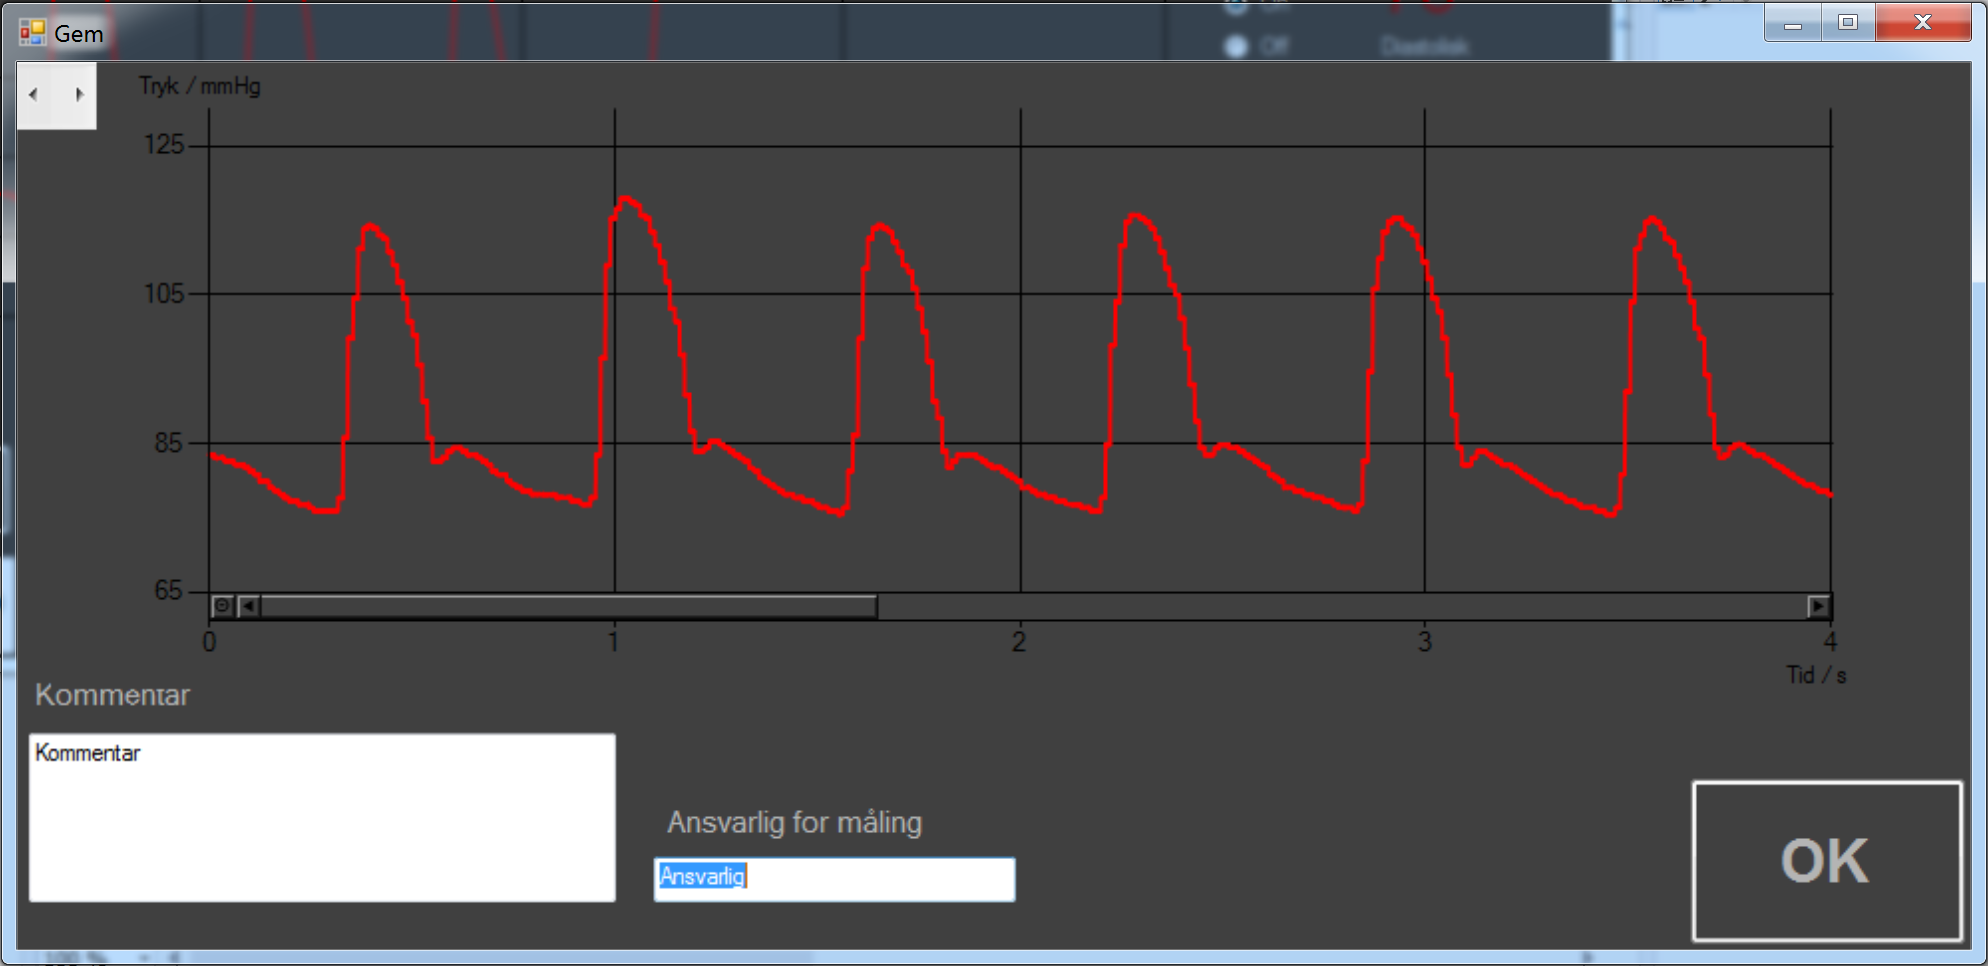
\includegraphics[width=1\textwidth]{Figurer/Pulstest_gemmevindue}
	\caption{Puls efter 10 sekunders måling}
\end{figure}

Det talte antal pulsslag holdes op mod dem, der er talt af metoden beregnpuls. Se pulsværdi i Figur 4.25.

\begin{figure}[H]
	\centering
	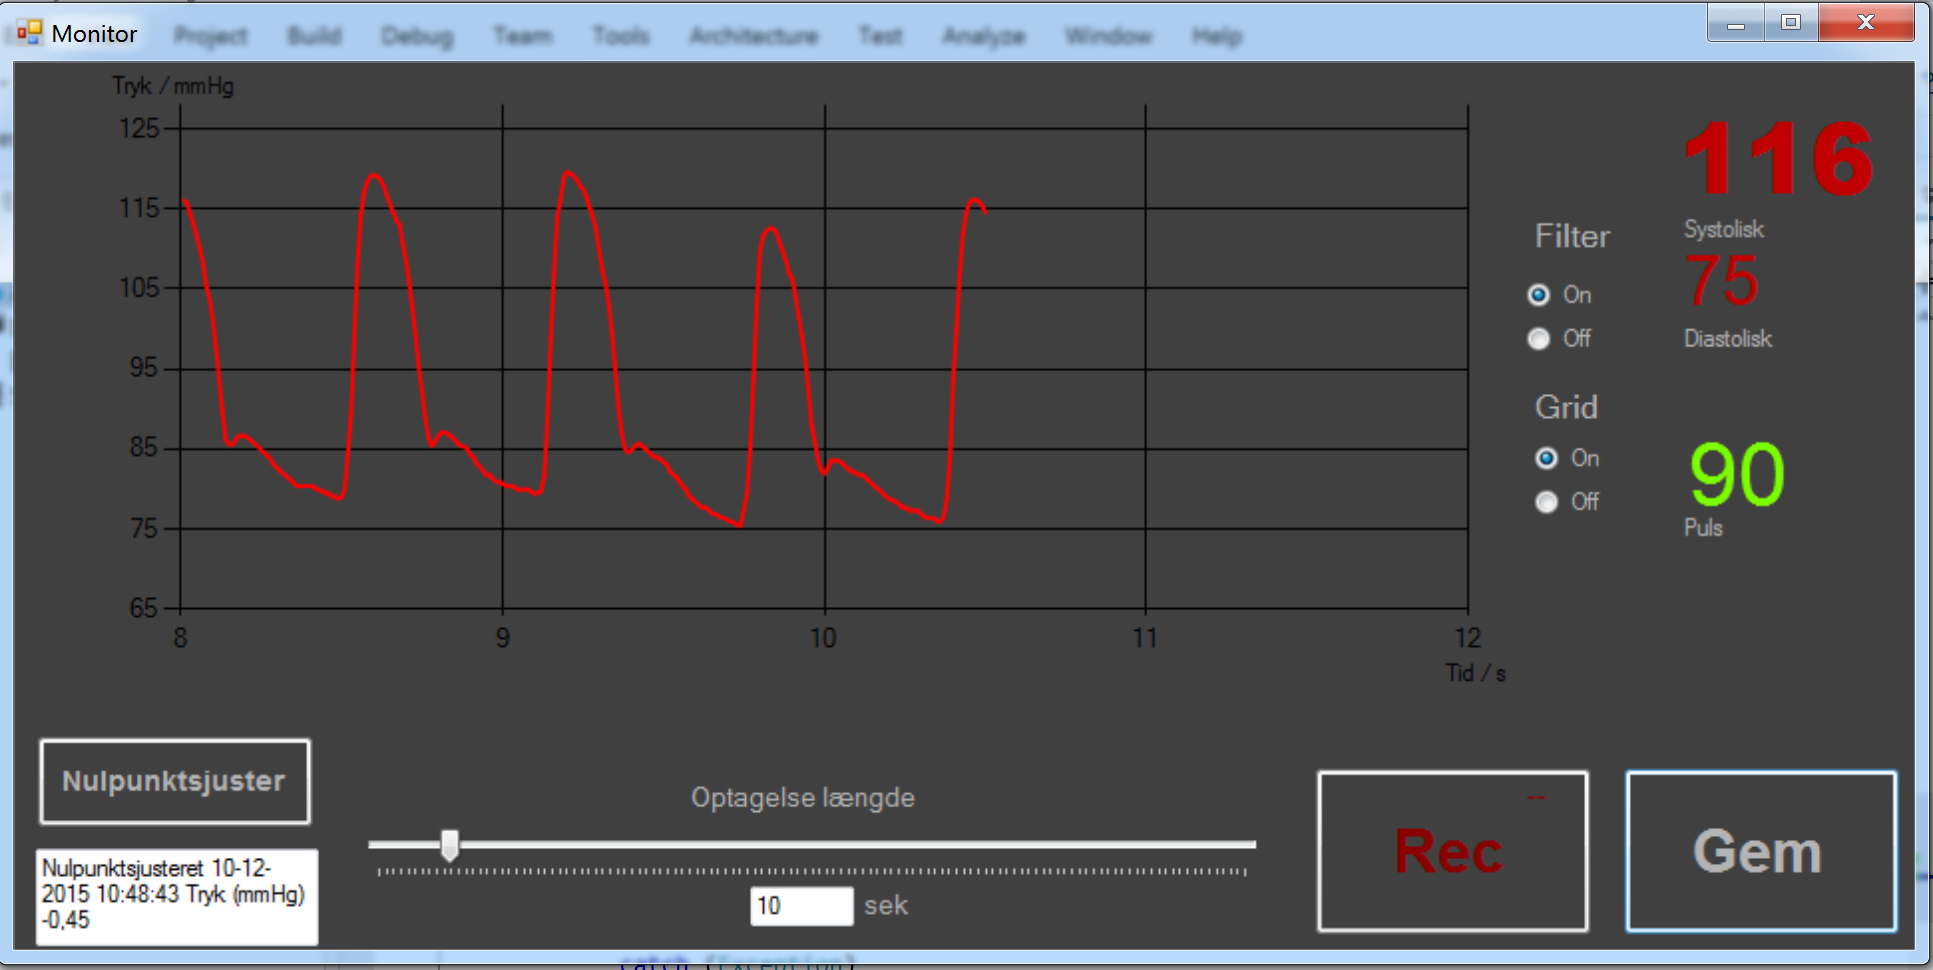
\includegraphics[width=1\textwidth]{Figurer/Pulstest_monitor}
	\caption{Puls efter 10 sekunders måling}
\end{figure}


Den beregnede puls er 90, hvilket stemmer overens med 15 pulsslag på 10 sekunder. Denne test kan bekræfte, at metoden fungerer efter hensigten.





\subsection{Use Case 3: Nulpunktsjuster}

Et DC-signal på 1 V bruges til inputsignal til DAQ. Se Figur 4.26.
\begin{figure}[H]
	\centering
	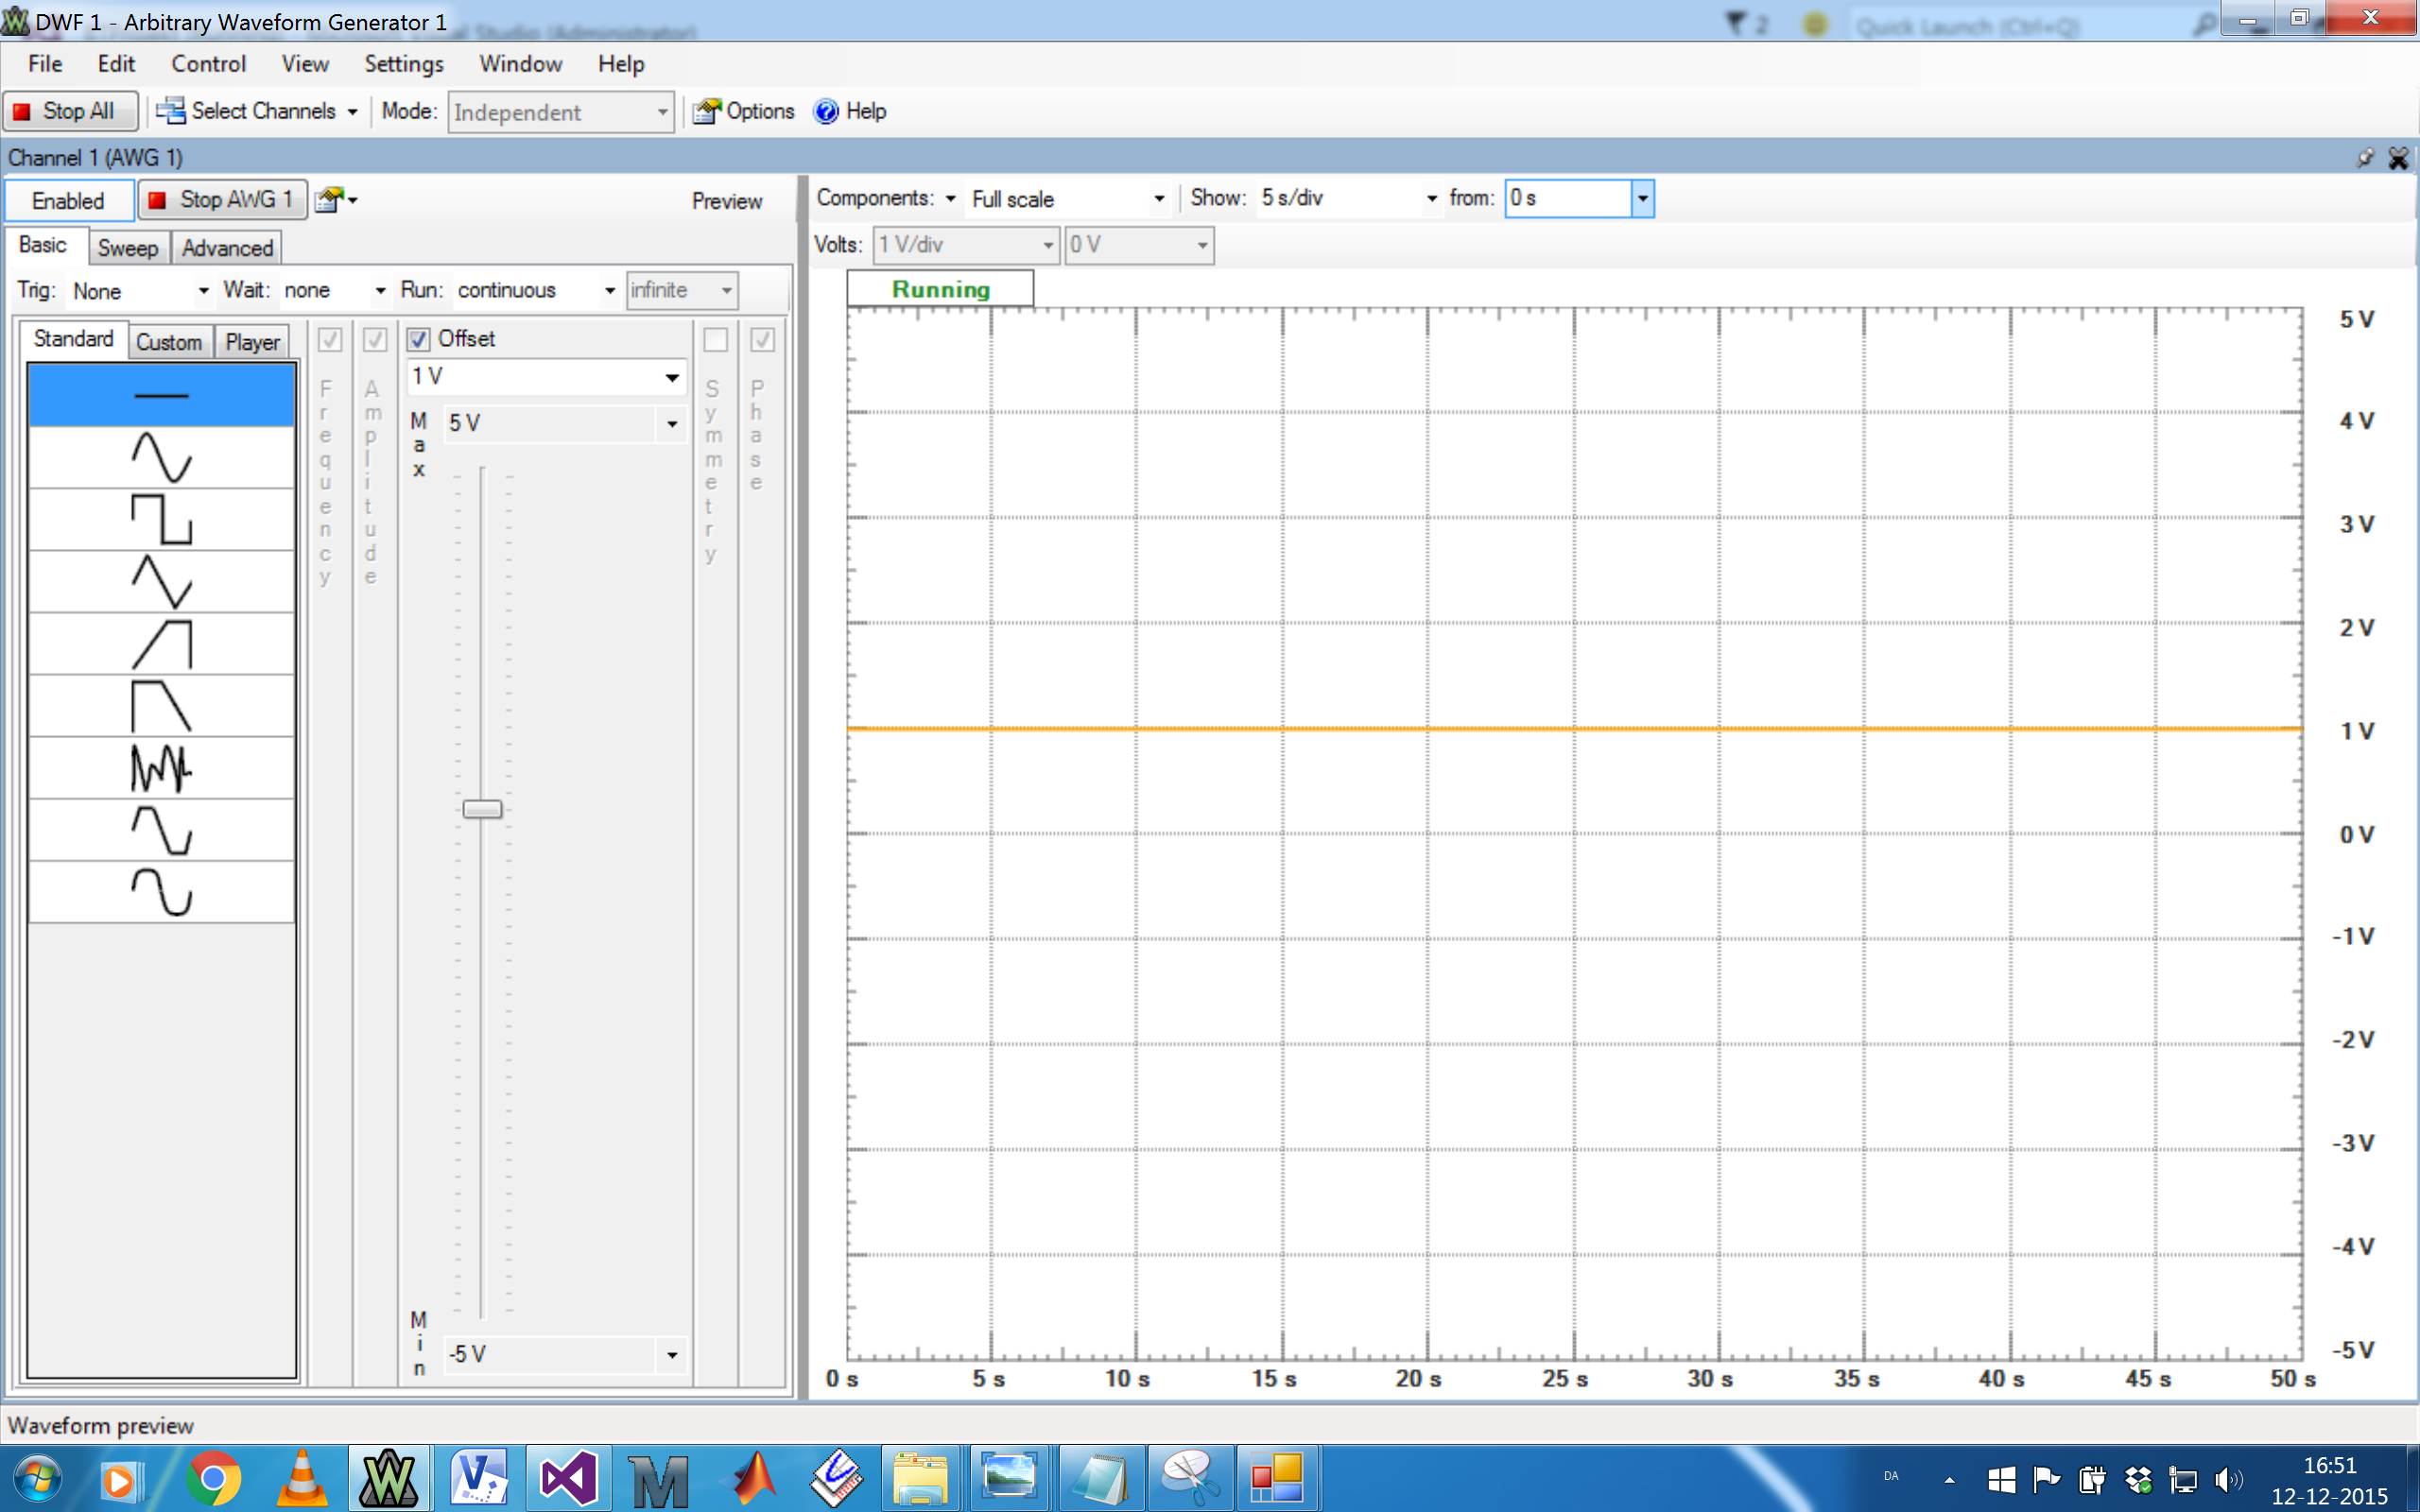
\includegraphics[width=1\textwidth]{Figurer/Test_Nul_1}
	\caption{Inputsignal til DAQ}
\end{figure}

Det ses at kalibreringskonstanten ligger på 57,9 og inputsignalet genererer det korrekte blodtryk. Se Figur 4.27.
\begin{figure}[H]
	\centering
	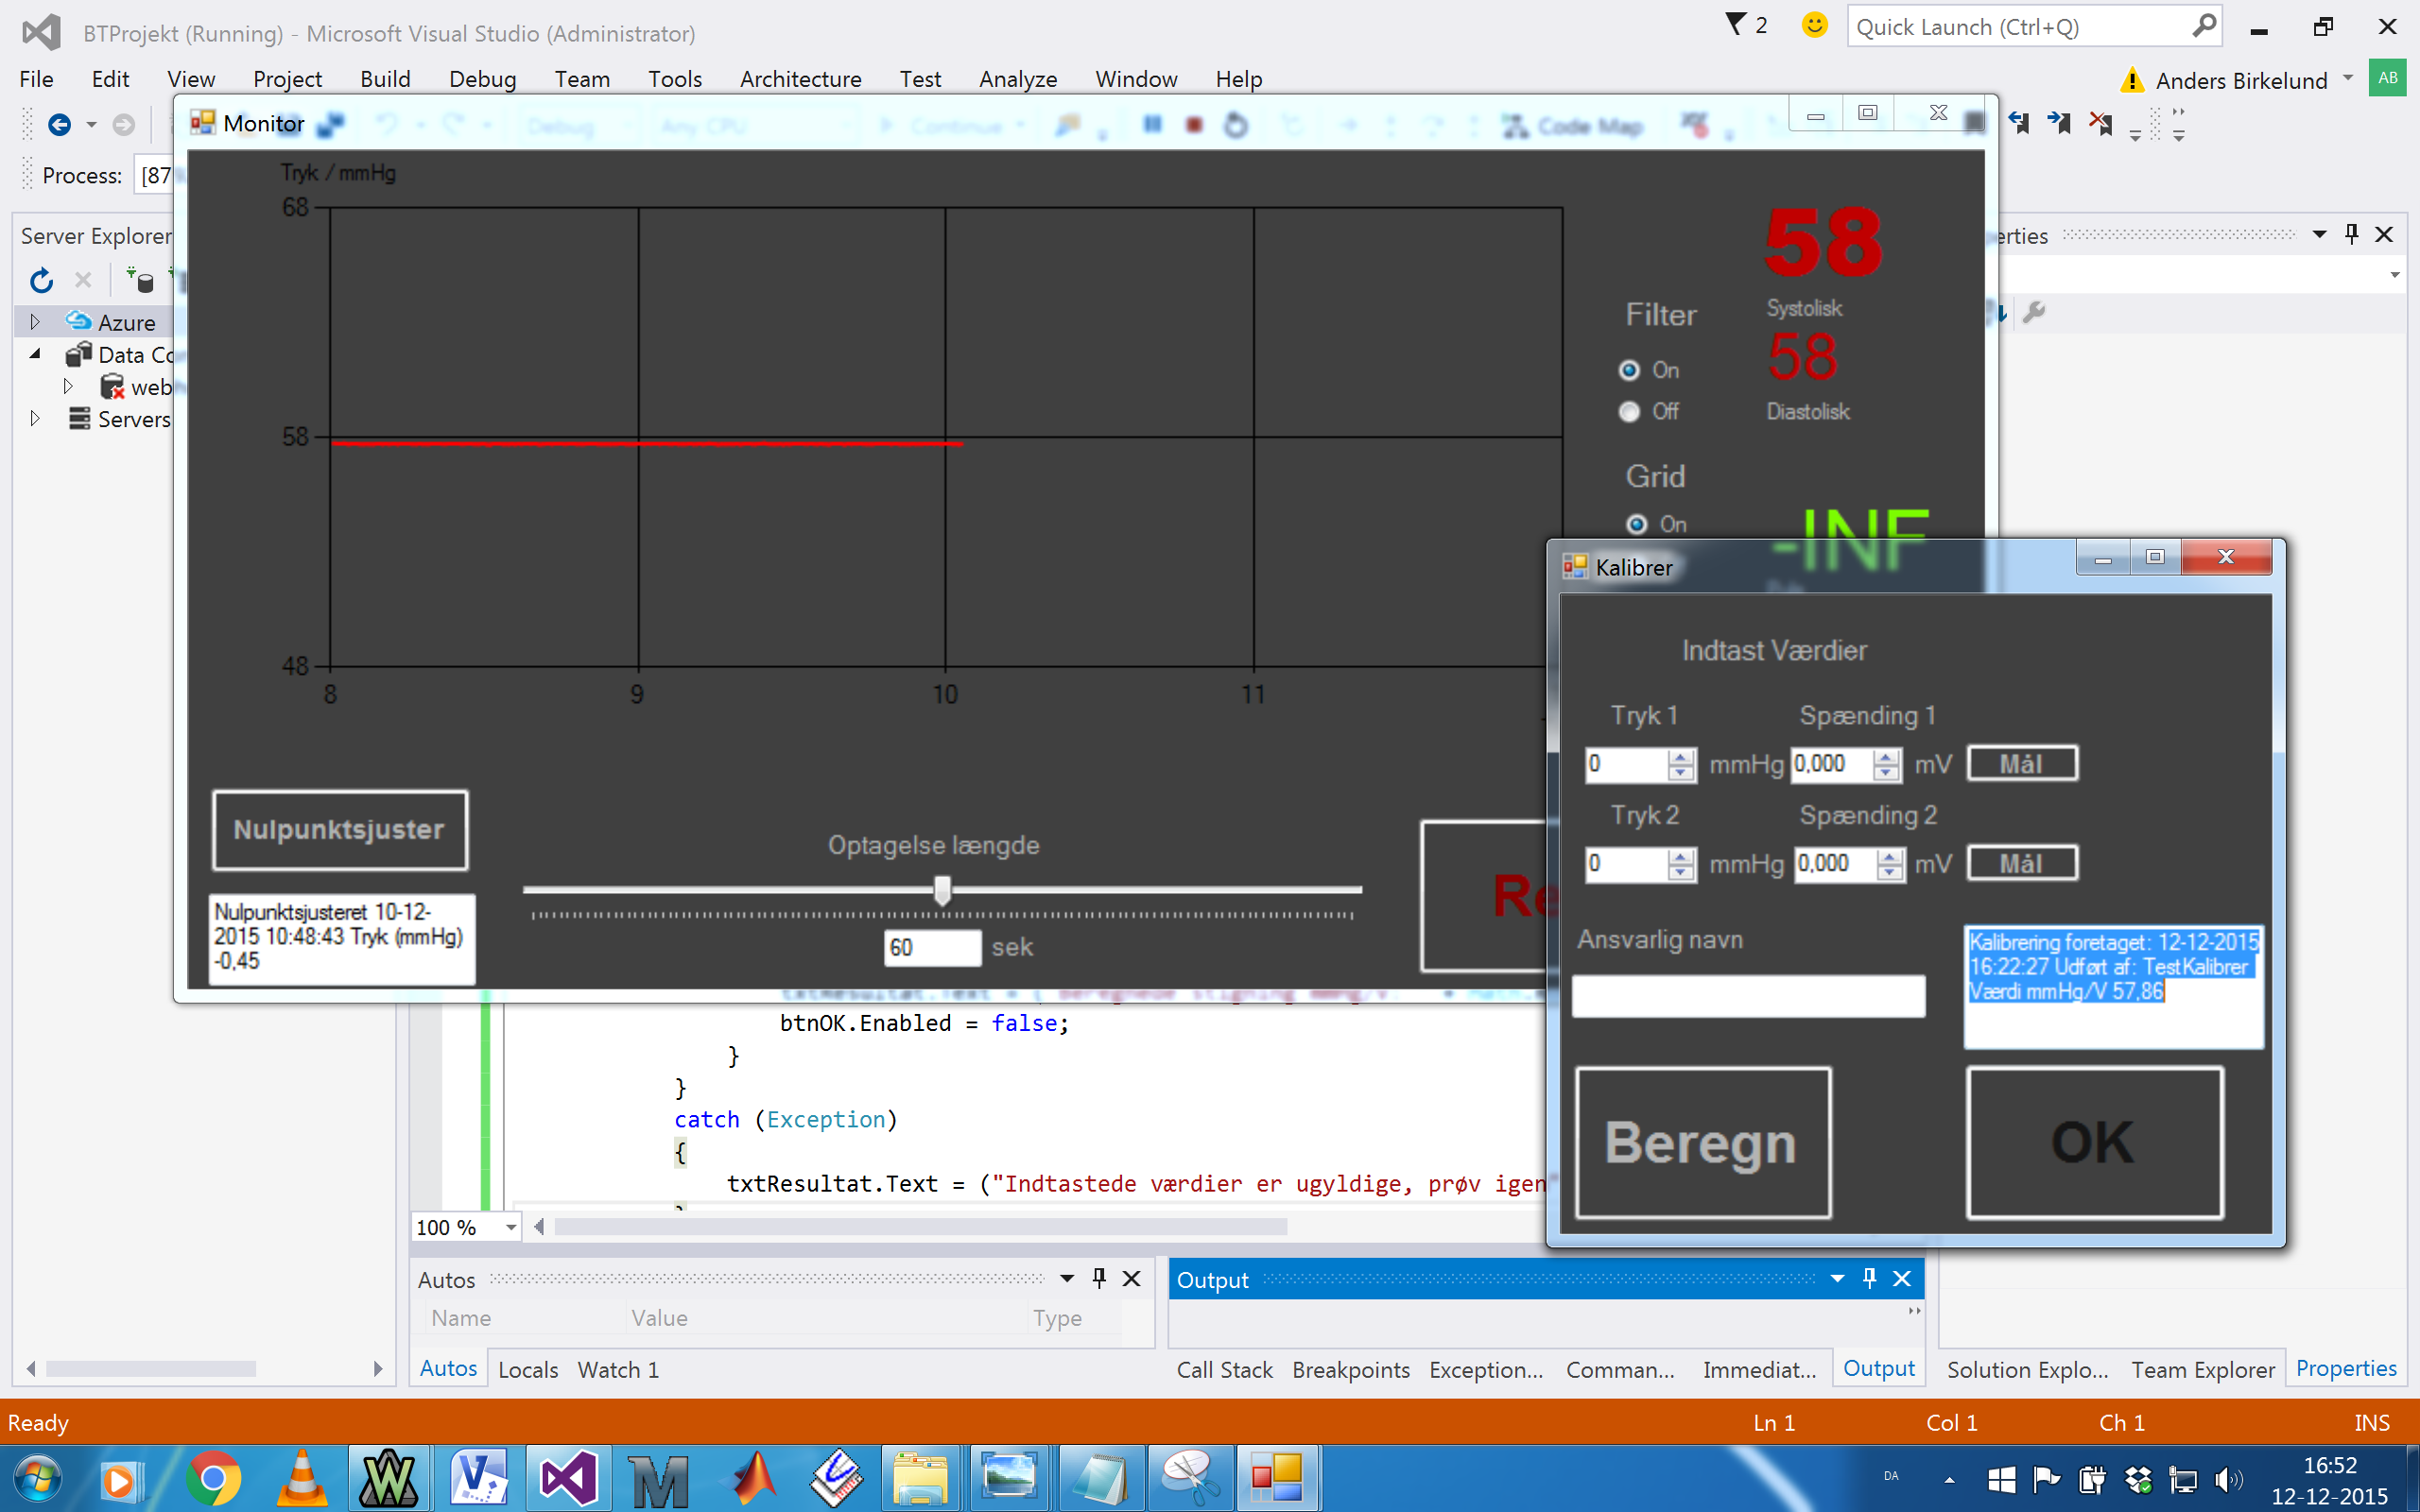
\includegraphics[width=1\textwidth]{Figurer/Test_Nul_2}
	\caption{Inputsignal til DAQ}
\end{figure}

Der trykkes på knappen "Nulpunktsjuster", og grafens værdi falder til 0. Se Figur 4.28.

\begin{figure}[H]
	\centering
	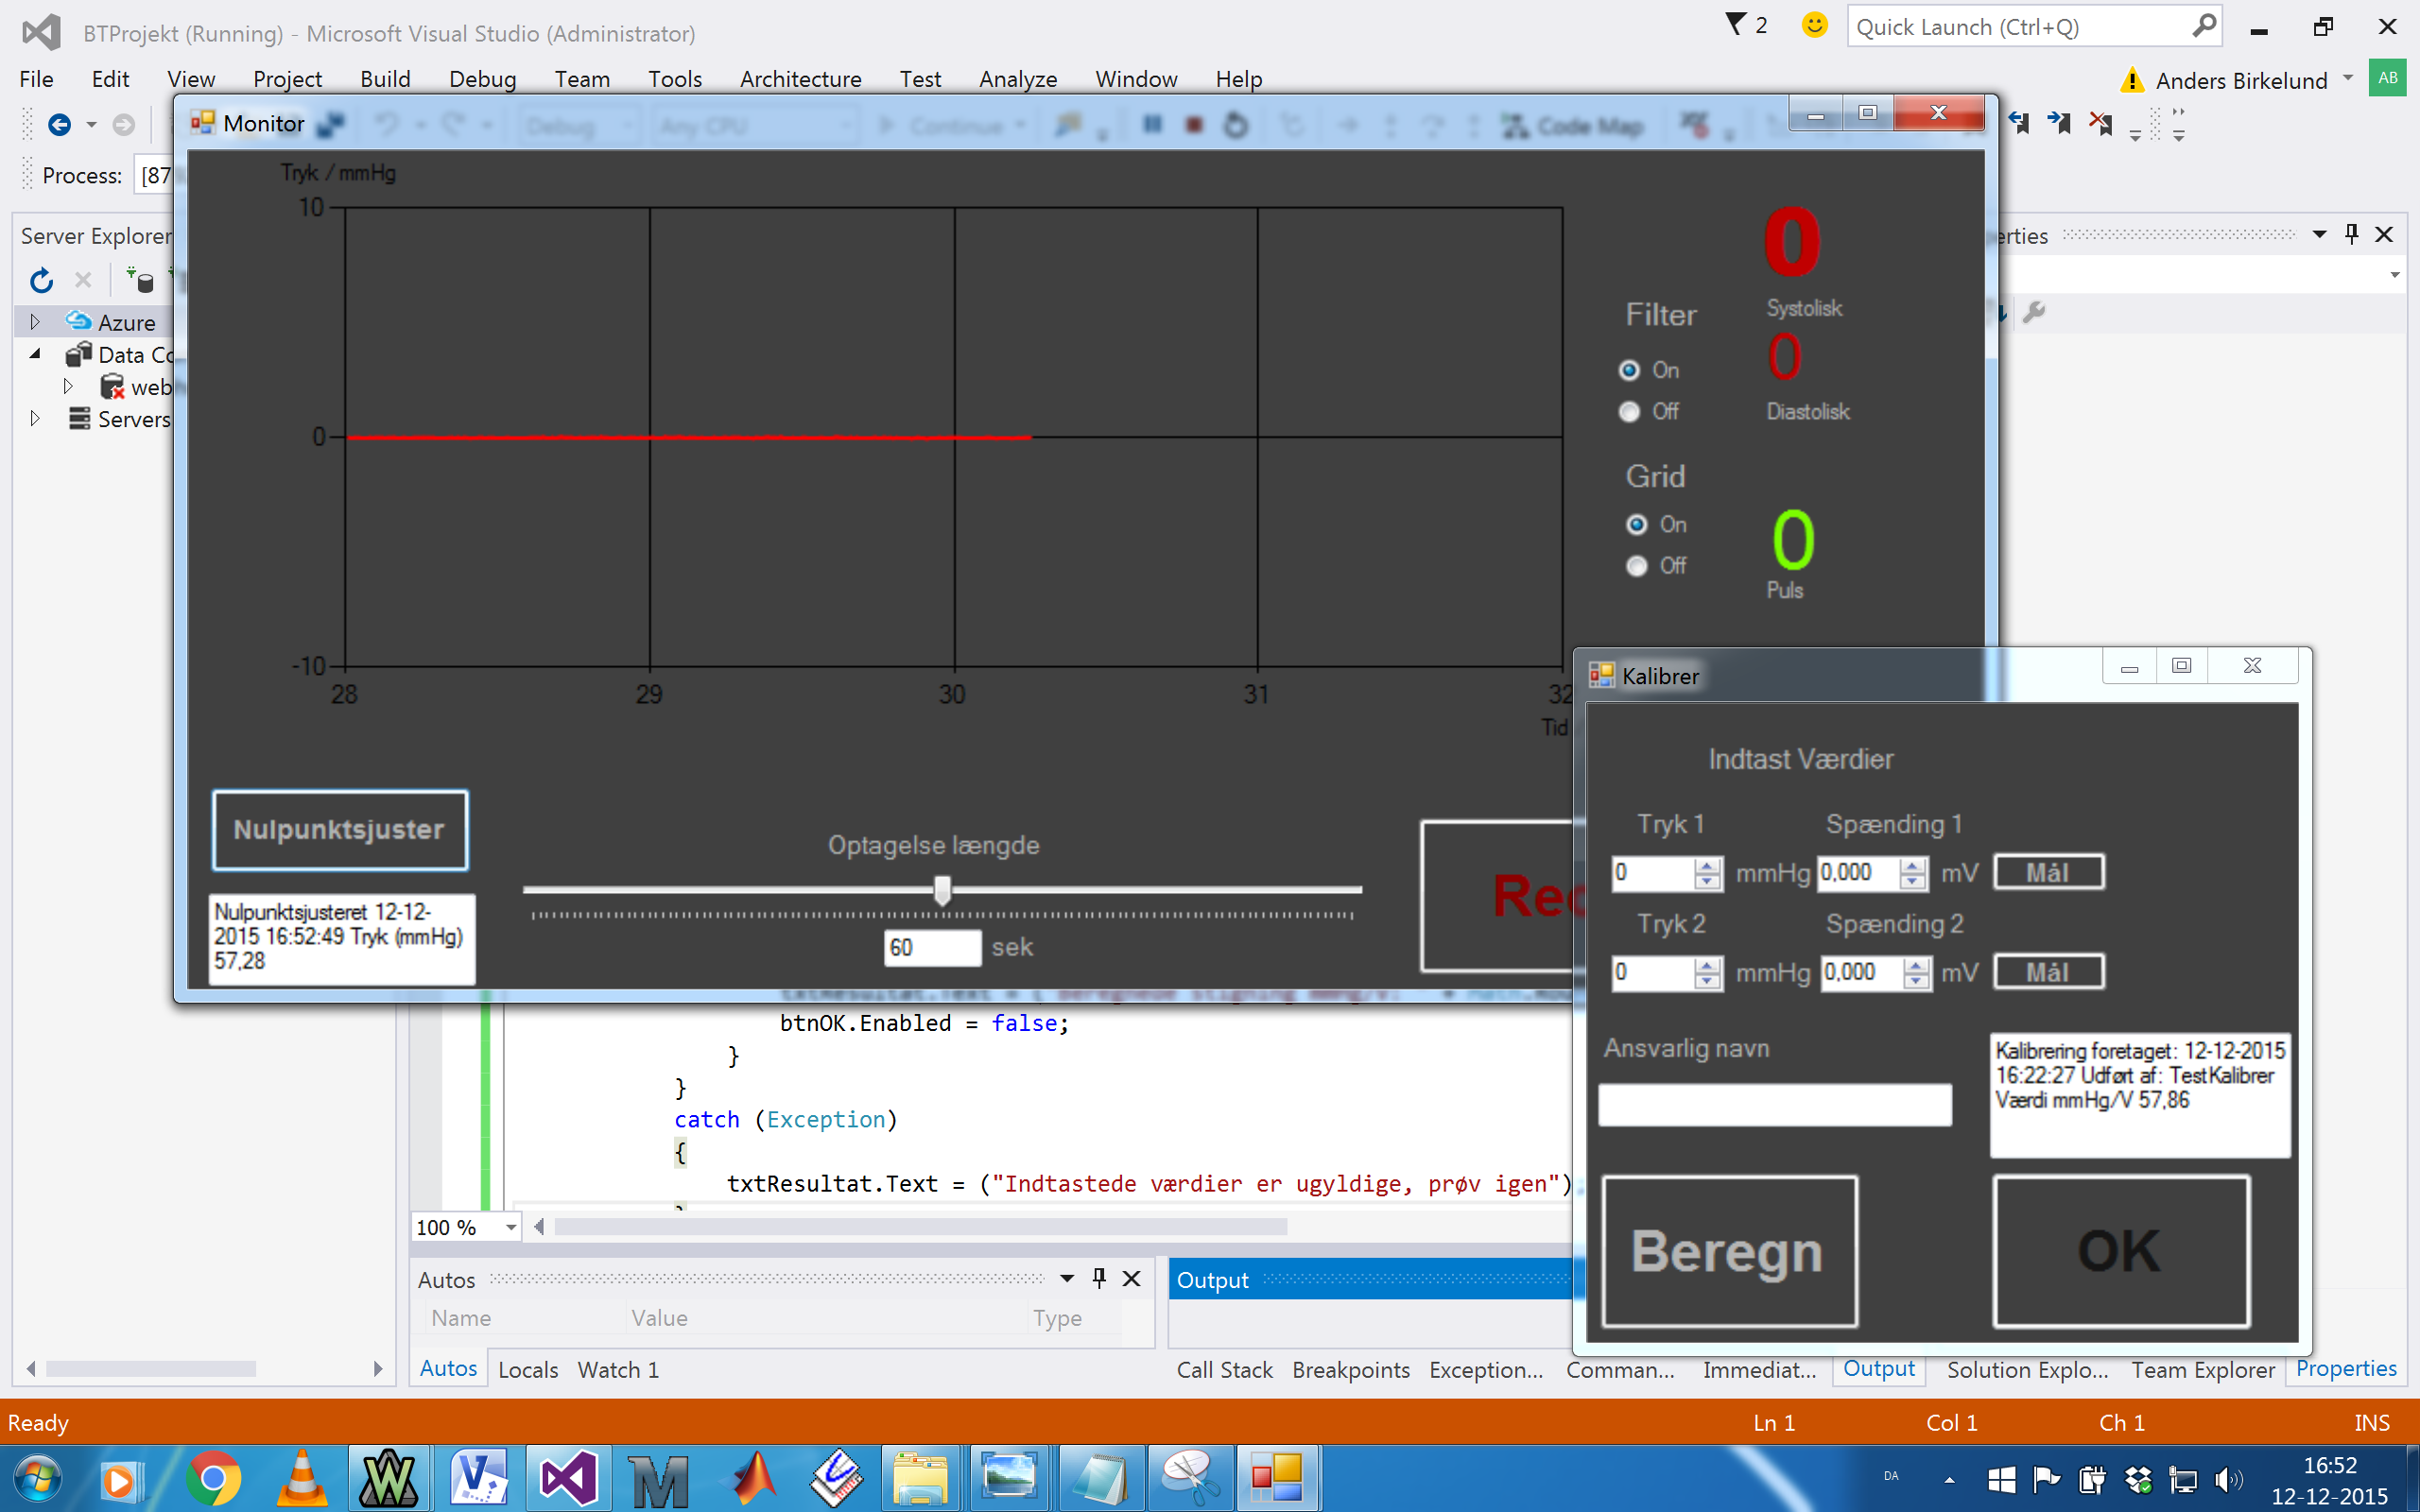
\includegraphics[width=1\textwidth]{Figurer/Test_Nul_3}
	\caption{Inputsignal til DAQ}
\end{figure}


\subsection{Use Case 4: Deaktiver filter}

Filteret er aktiveret, og det filtrerede signal vises i graf. Se Figur 4.29.

\begin{figure}[H]
	\centering
	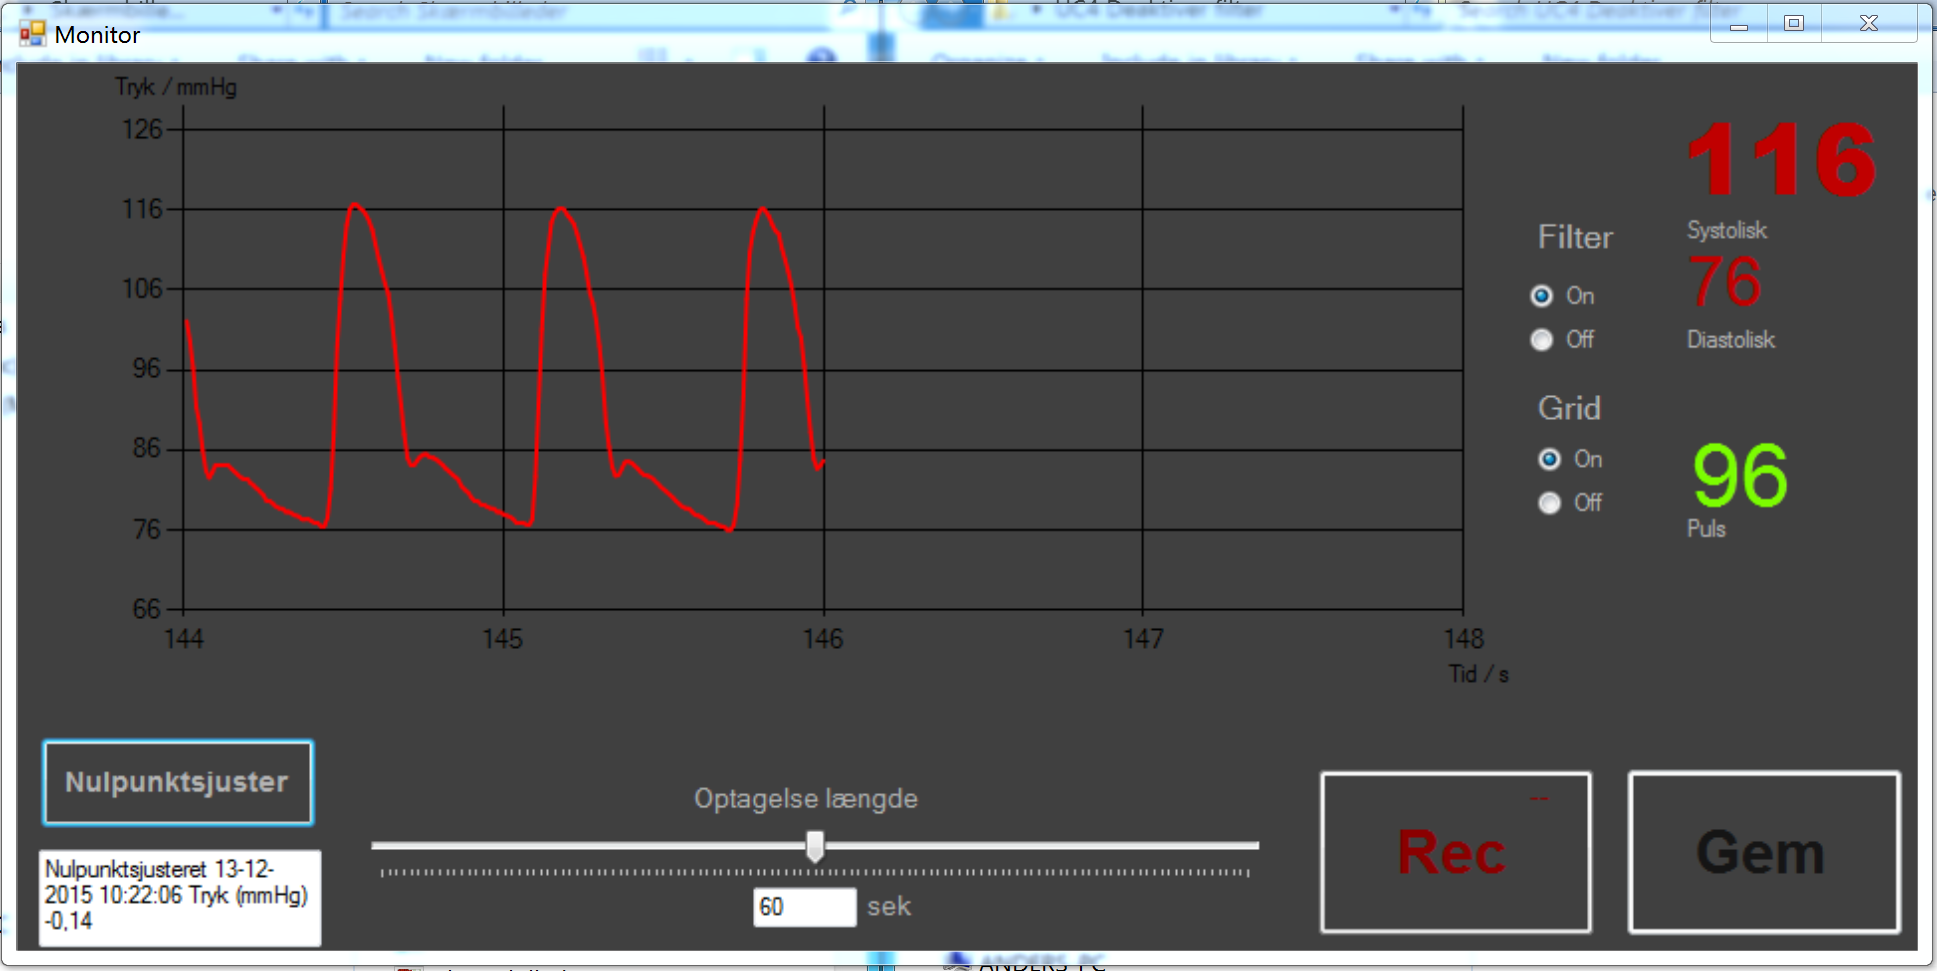
\includegraphics[width=1\textwidth]{Figurer/Test_Deaktiver_1}
	\caption{Målingen vises med filter aktiveret}
\end{figure}

I Beregninger klassen beregnes målingen der udskrives på graf med filter, da bool'en 'filterOn' er 'true. Se Figur 4.30.

\begin{figure}[H]
	\centering
	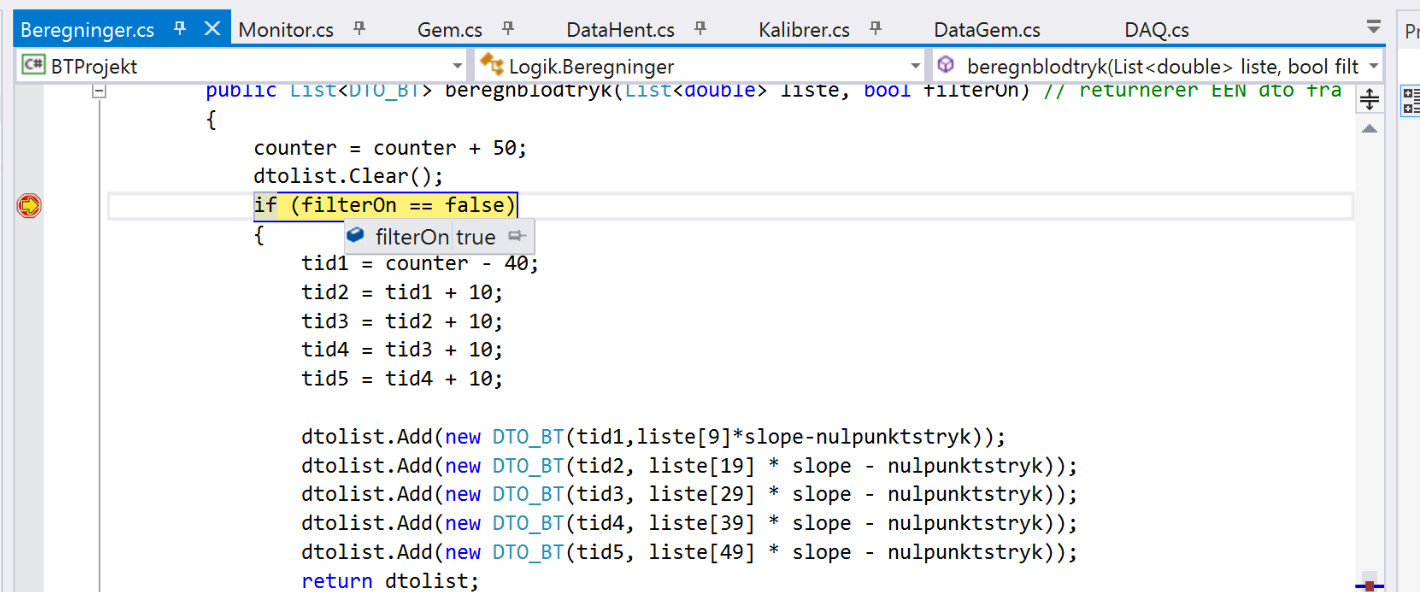
\includegraphics[width=1\textwidth]{Figurer/Test_Deaktiver_2}
	\caption{Beregningerklassen opretter filtrerede DTO'er}
\end{figure}

Der trykkes på radiobutton "Off"\ under "Filter"\ og bool'en der sendes med metoden "beregnBlodtryk"\ sættes til 'false'. Metoden beregner blodtrykket der udskrives i Monitor-vinduet, uden filter. Se Figur 4.31.

\begin{figure}[H]
	\centering
	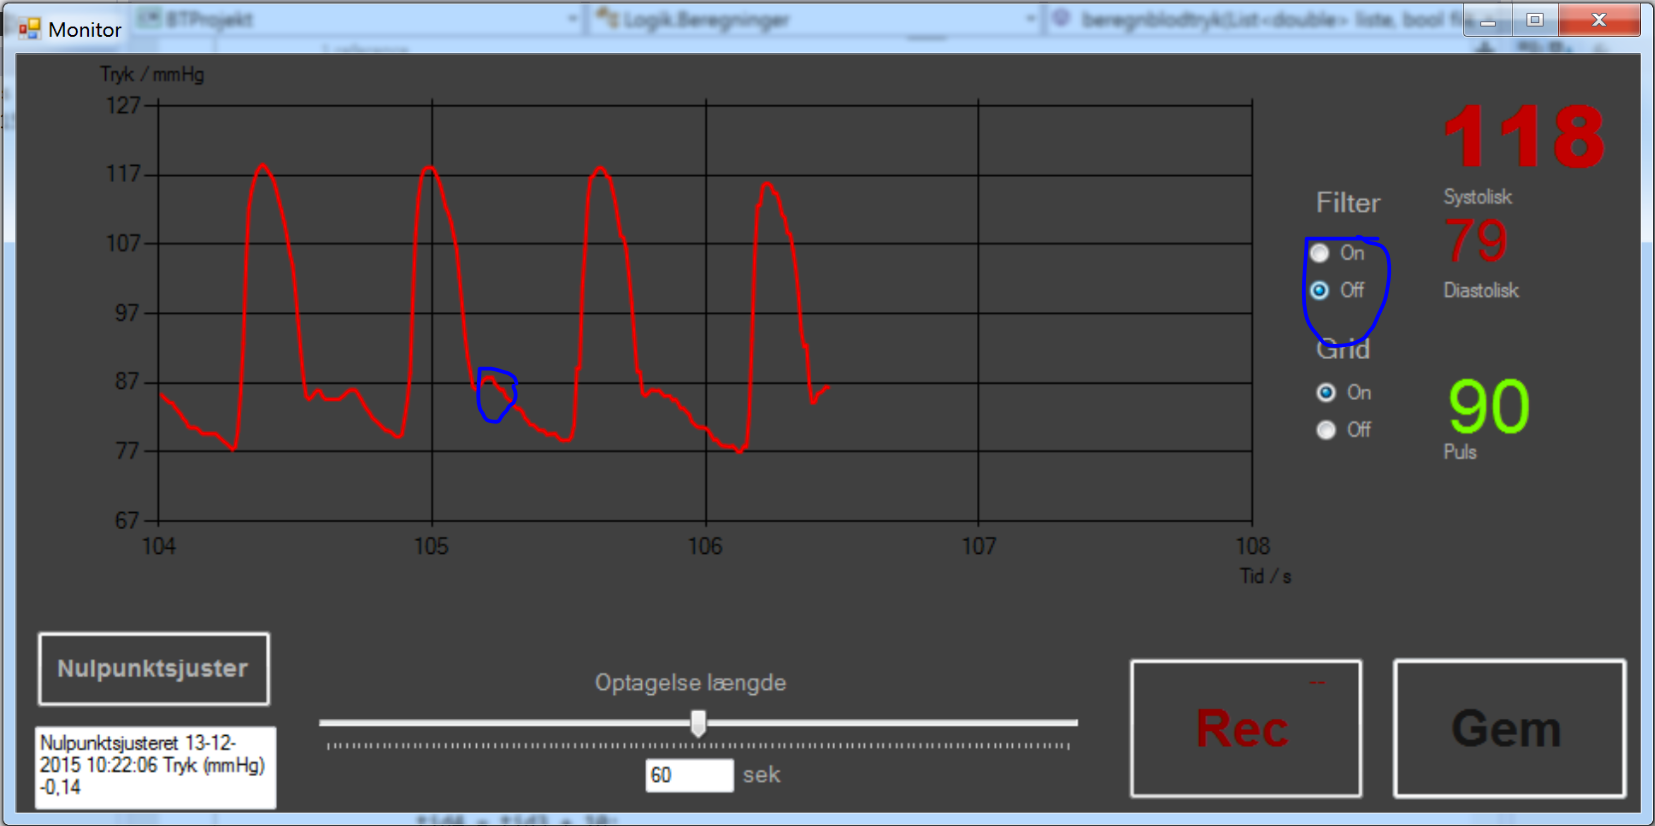
\includegraphics[width=1\textwidth]{Figurer/Test_Deaktiver_3}
	\caption{Blodtrykssignal før og efter deaktivering af filter. Den blå markering viser overgangen}
\end{figure}

Beregningerklassen kører metoden uden filter, da "filterOn"\ er 'false'. Se Figur 4.32.

\begin{figure}[H]
	\centering
	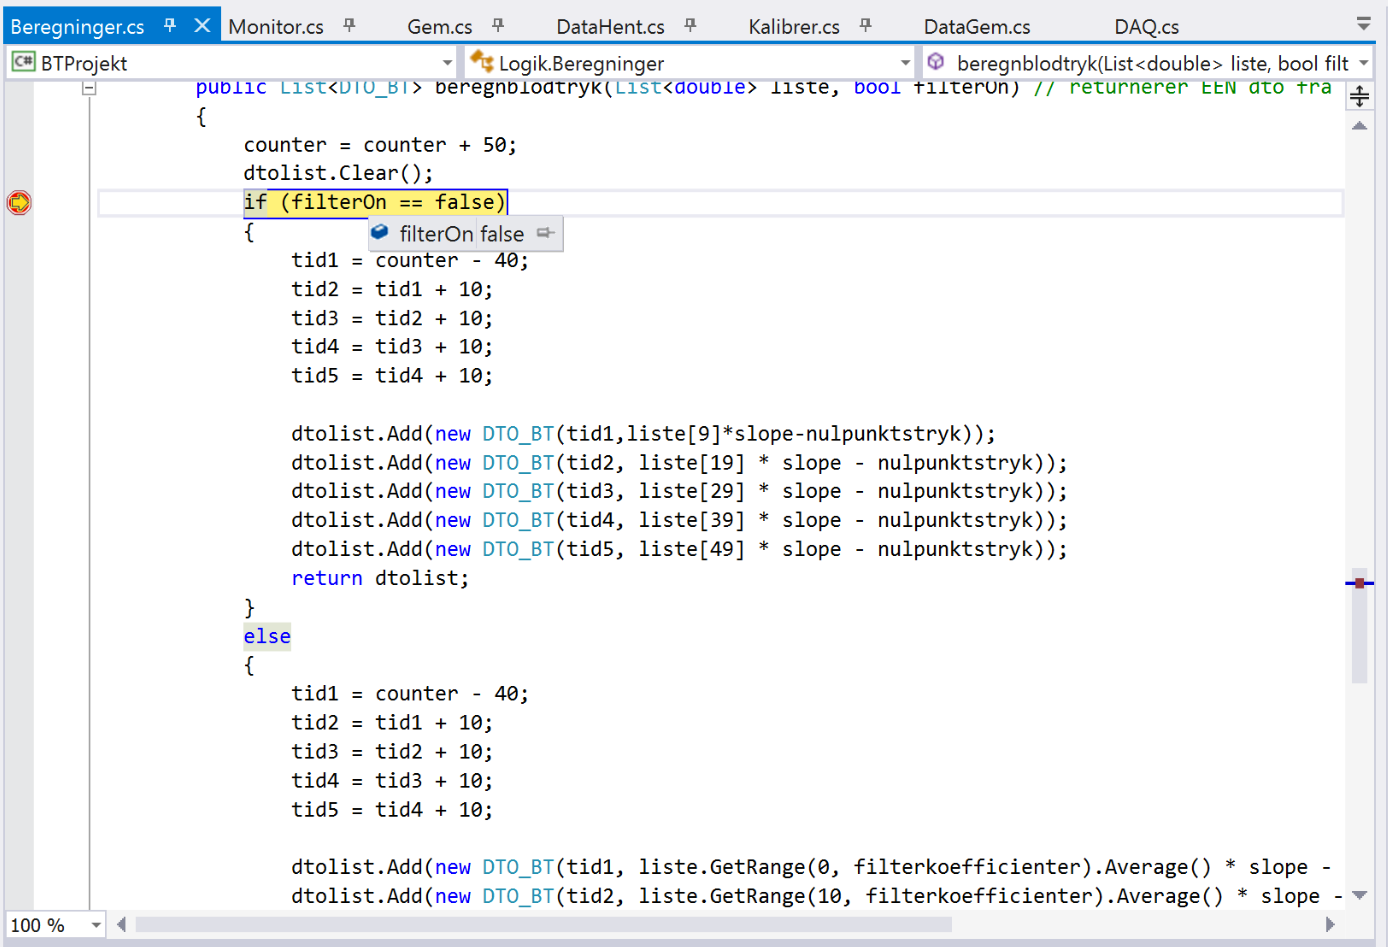
\includegraphics[width=1\textwidth]{Figurer/Test_Deaktiver_4}
	\caption{Beregningerklassen opretter ufiltrerede DTO'er}
\end{figure}

\subsection{Use Case 5: Aktiver filter}

Filteret er ikke aktiveret, og det ufiltrerede signal udskrives. Se Figur 4.33.

\begin{figure}[H]
	\centering
	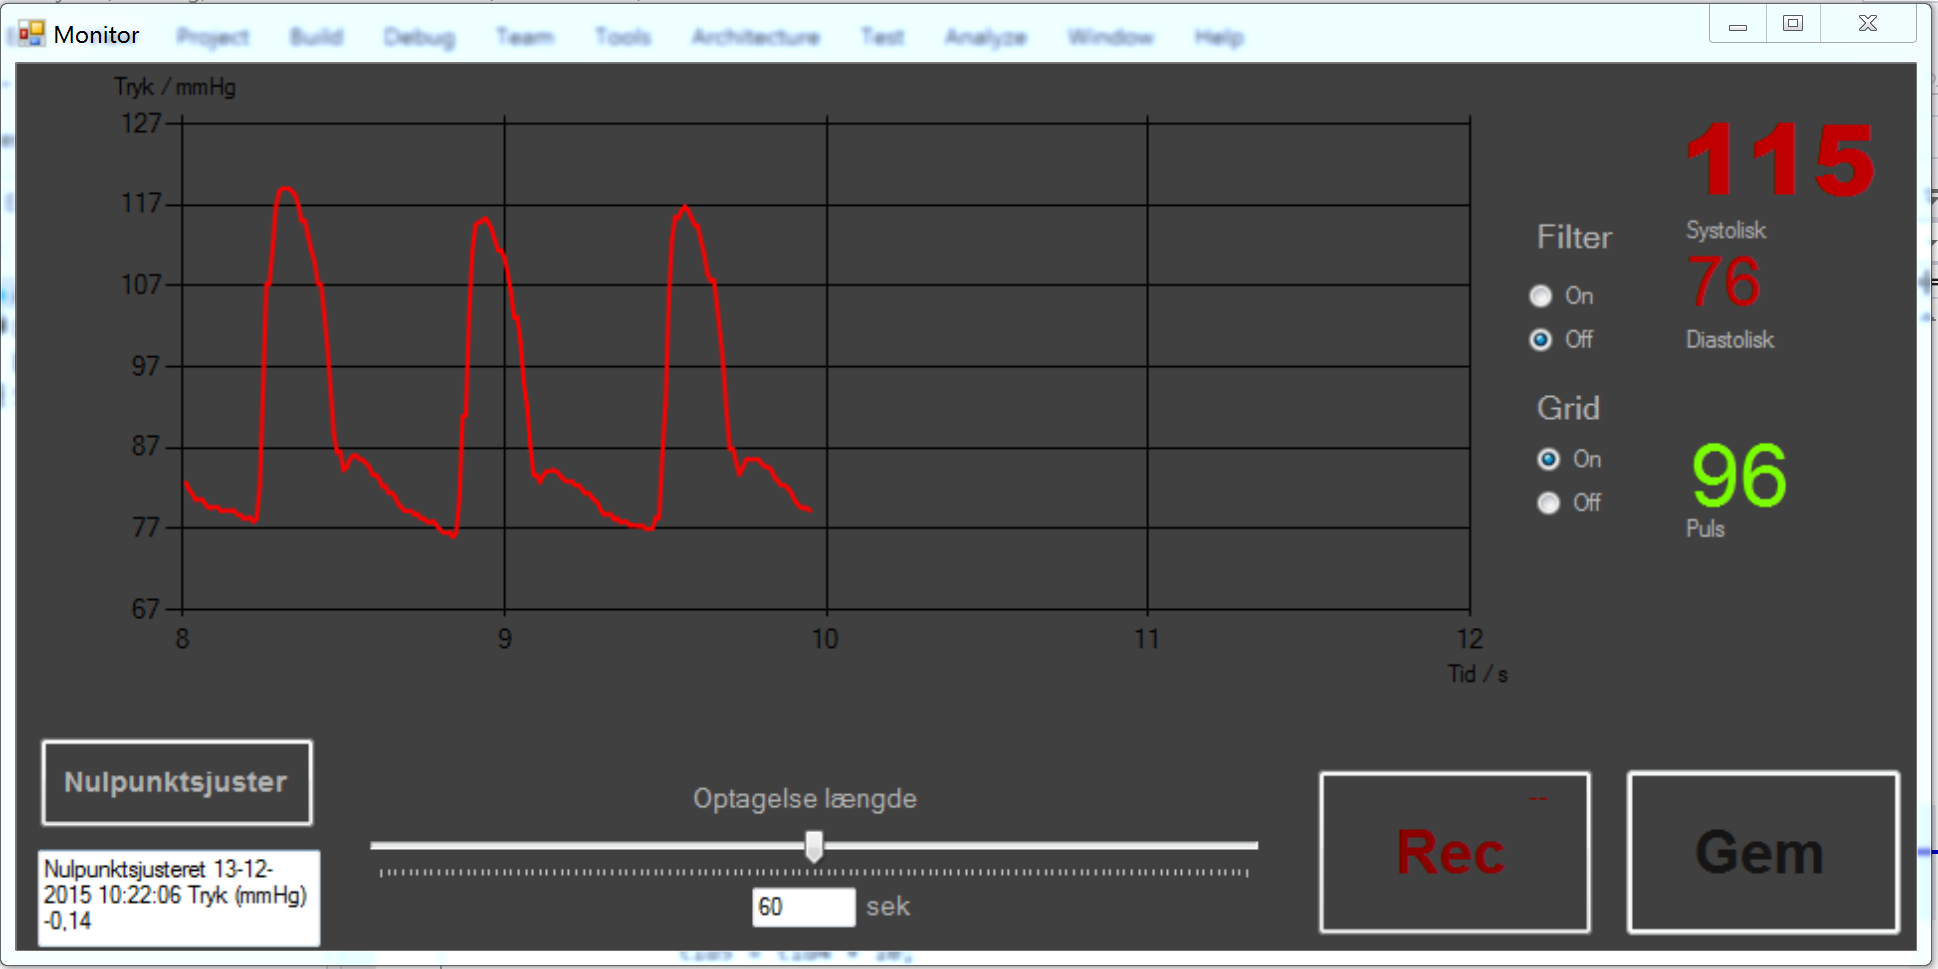
\includegraphics[width=1\textwidth]{Figurer/Test_Aktiver_1}
	\caption{Ufiltreret signal udskrives i graf}
\end{figure}

I Beregninger klassen beregnes målingen der udskrives på graf uden filter, da bool'en "filterOn"\ er 'false'. Se Figur 4.34.

\begin{figure}[H]
	\centering
	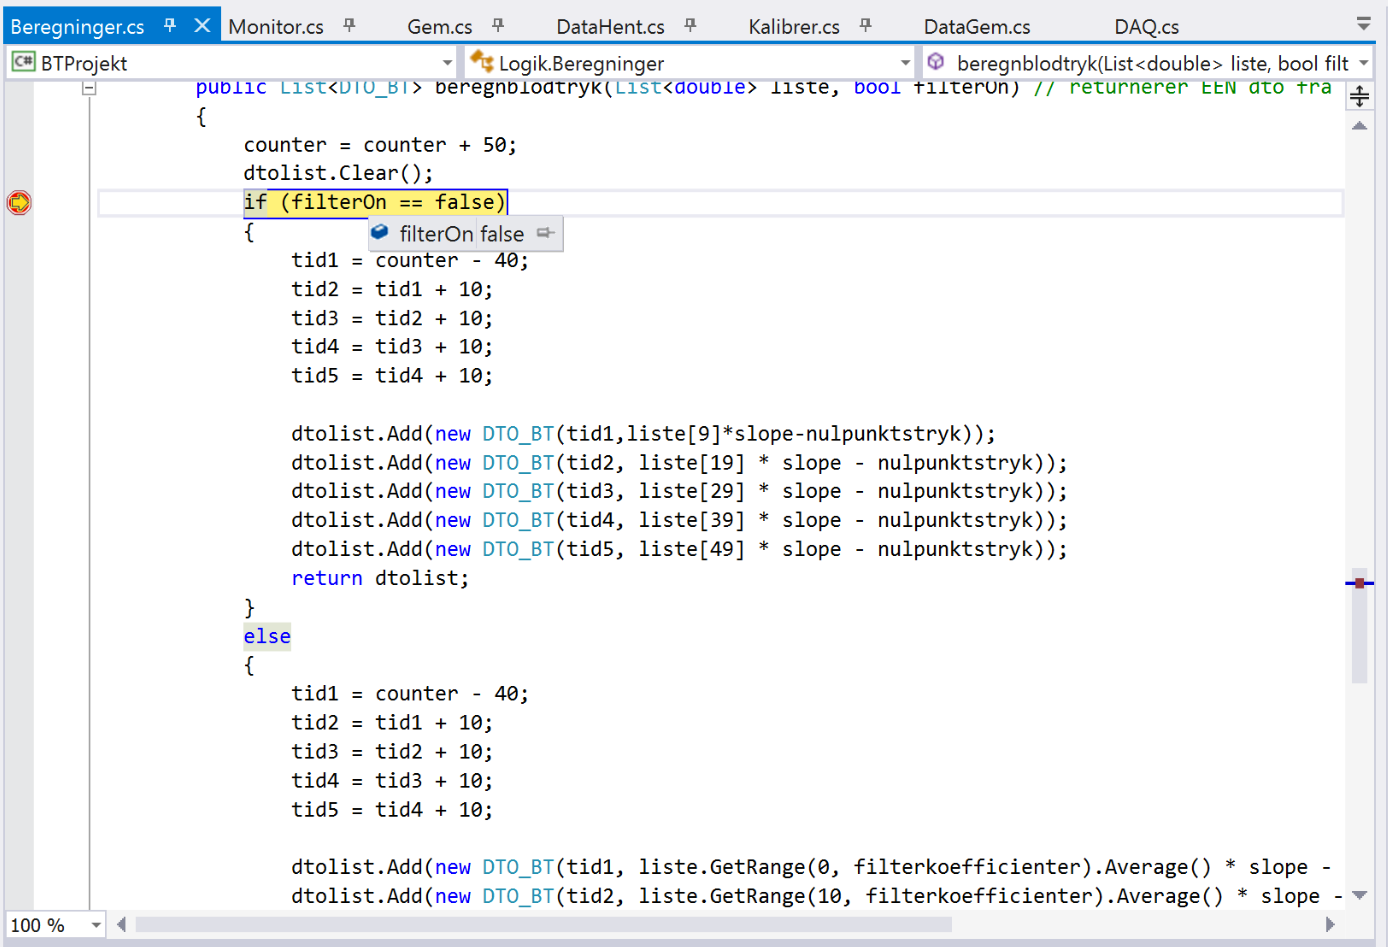
\includegraphics[width=1\textwidth]{Figurer/Test_Aktiver_2}
	\caption{Beregningerklassen opretter ufiltrerede}
\end{figure}

Der trykkes på "On"\ under "Filter"\ og det ses at det udskrevne signal filtreres. Se Figur 4.35.

\begin{figure}[H]
	\centering
	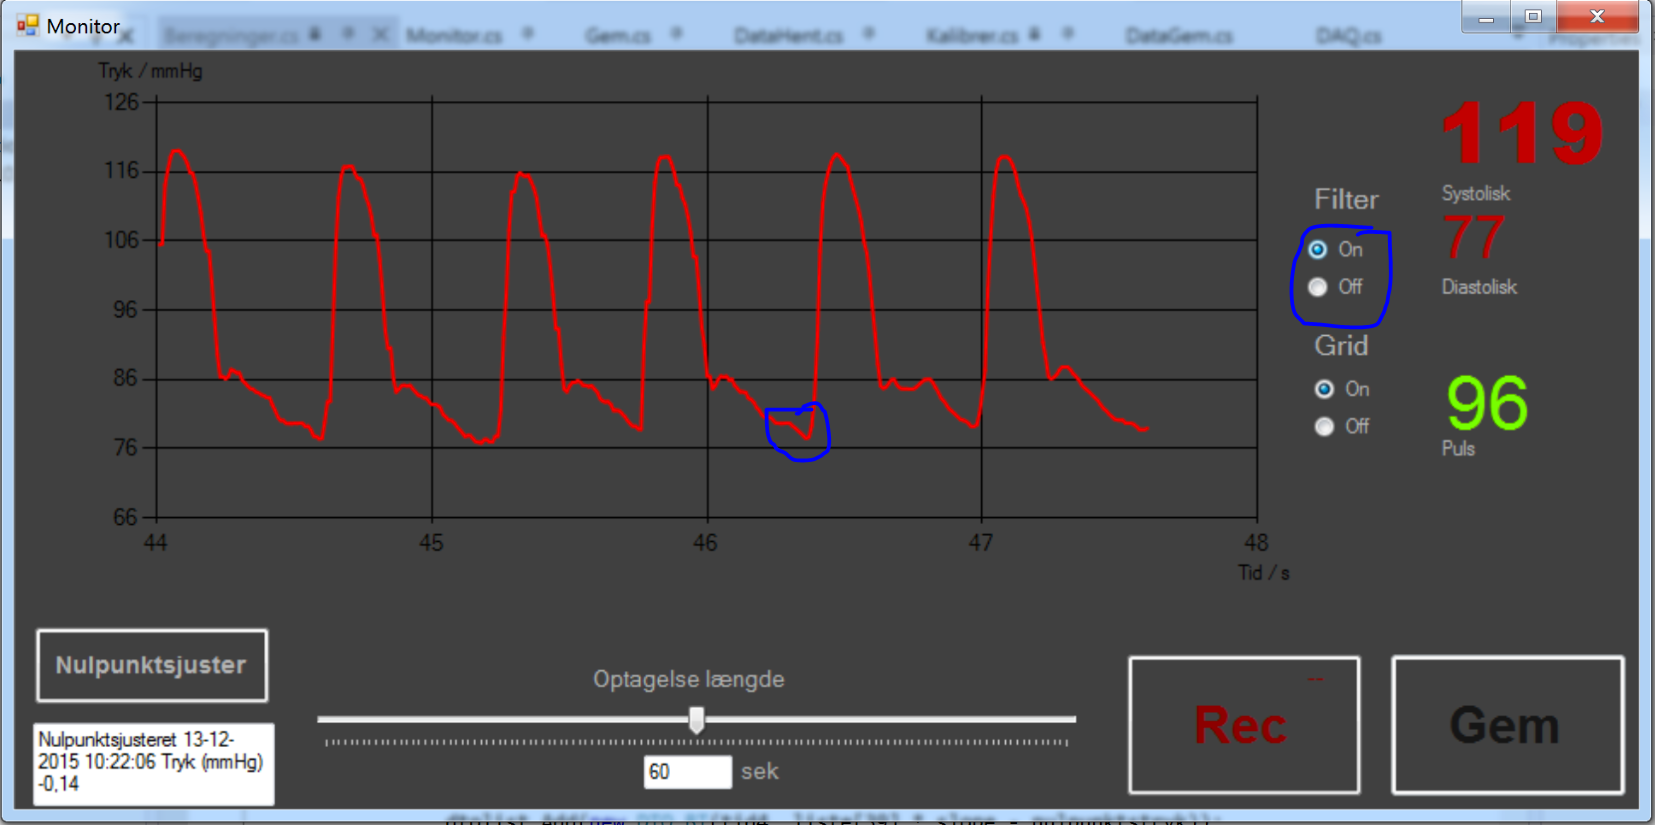
\includegraphics[width=1\textwidth]{Figurer/Test_Aktiver_3}
	\caption{Filtreret signal udskrives i graf efter markering med blå cirkel}
\end{figure}

I beregninger klassen er bool'en der sendes med metoden "beregnBlodtryk"\ sat til 'true'. Metoden beregner blodtrykket, der udskrives i Monitor-vinduet, med filter. Se Figur 4.36.

\begin{figure}[H]
	\centering
	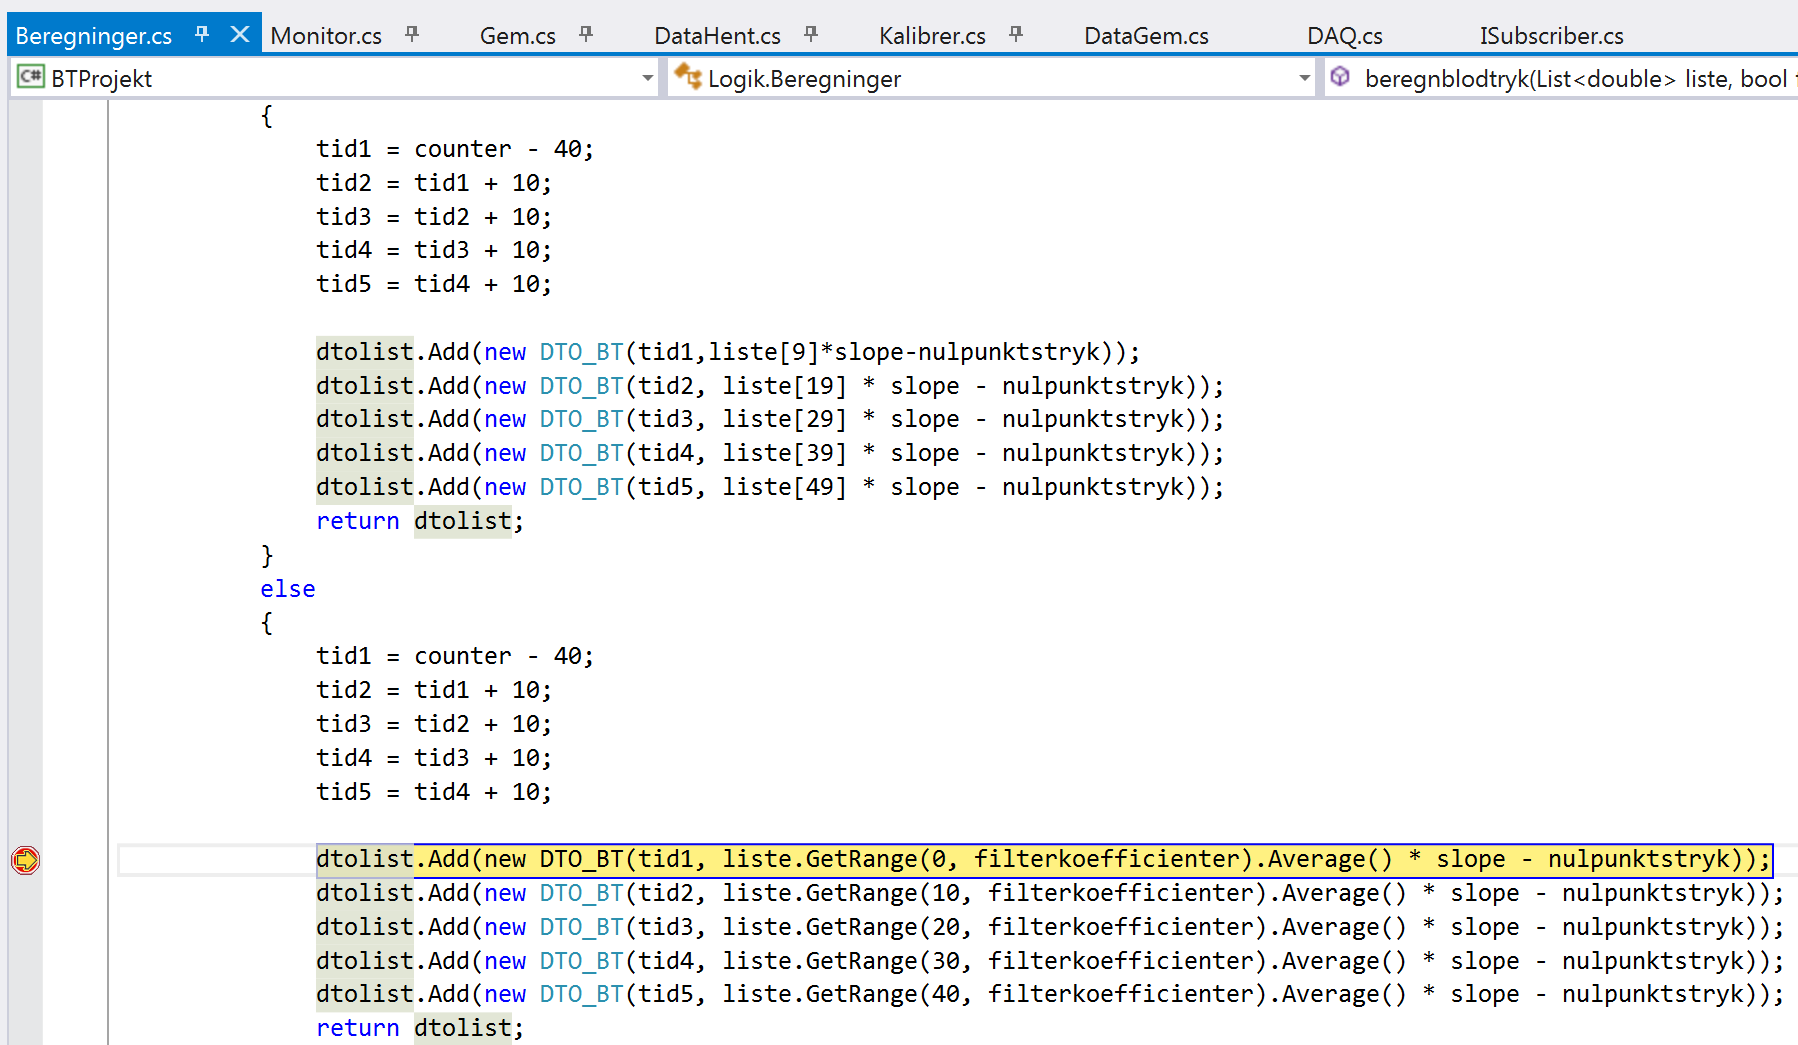
\includegraphics[width=1\textwidth]{Figurer/Test_Aktiver_4}
	\caption{Beregningerklassen opretter filtrerede DTO'er}
\end{figure}

\subsection{Use Case 6: Gem måling}
Kalibreringskonstant (mmHg/V) og nulpunktsværdi (mmHg) for måling fremgår af Figur 4.37.
\begin{figure}[H]
	\centering
	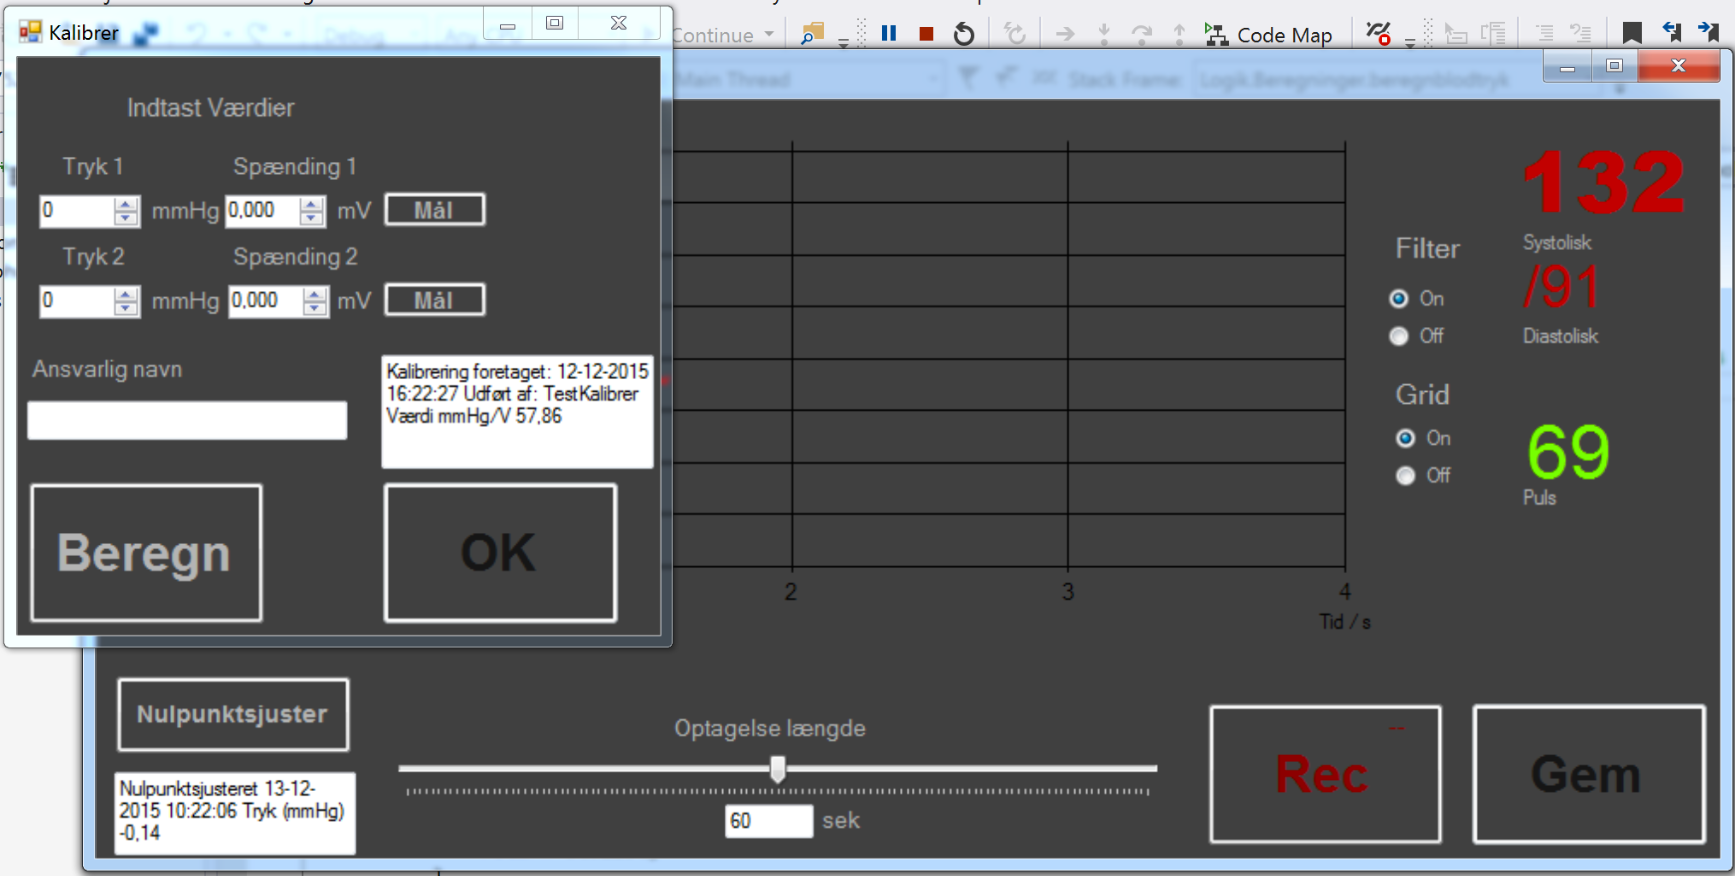
\includegraphics[width=1\textwidth]{Figurer/UC6_InitialConditions}
	\caption{Monitor-vinduets initiale værdier (kalibreringskonstant og nulpunktstryk)}
\end{figure}
 
Forsker vælger målelængde til fem sekunder og trykker på "Rec". Se Figur 4.38.
 
\begin{figure}[H]
	\centering
	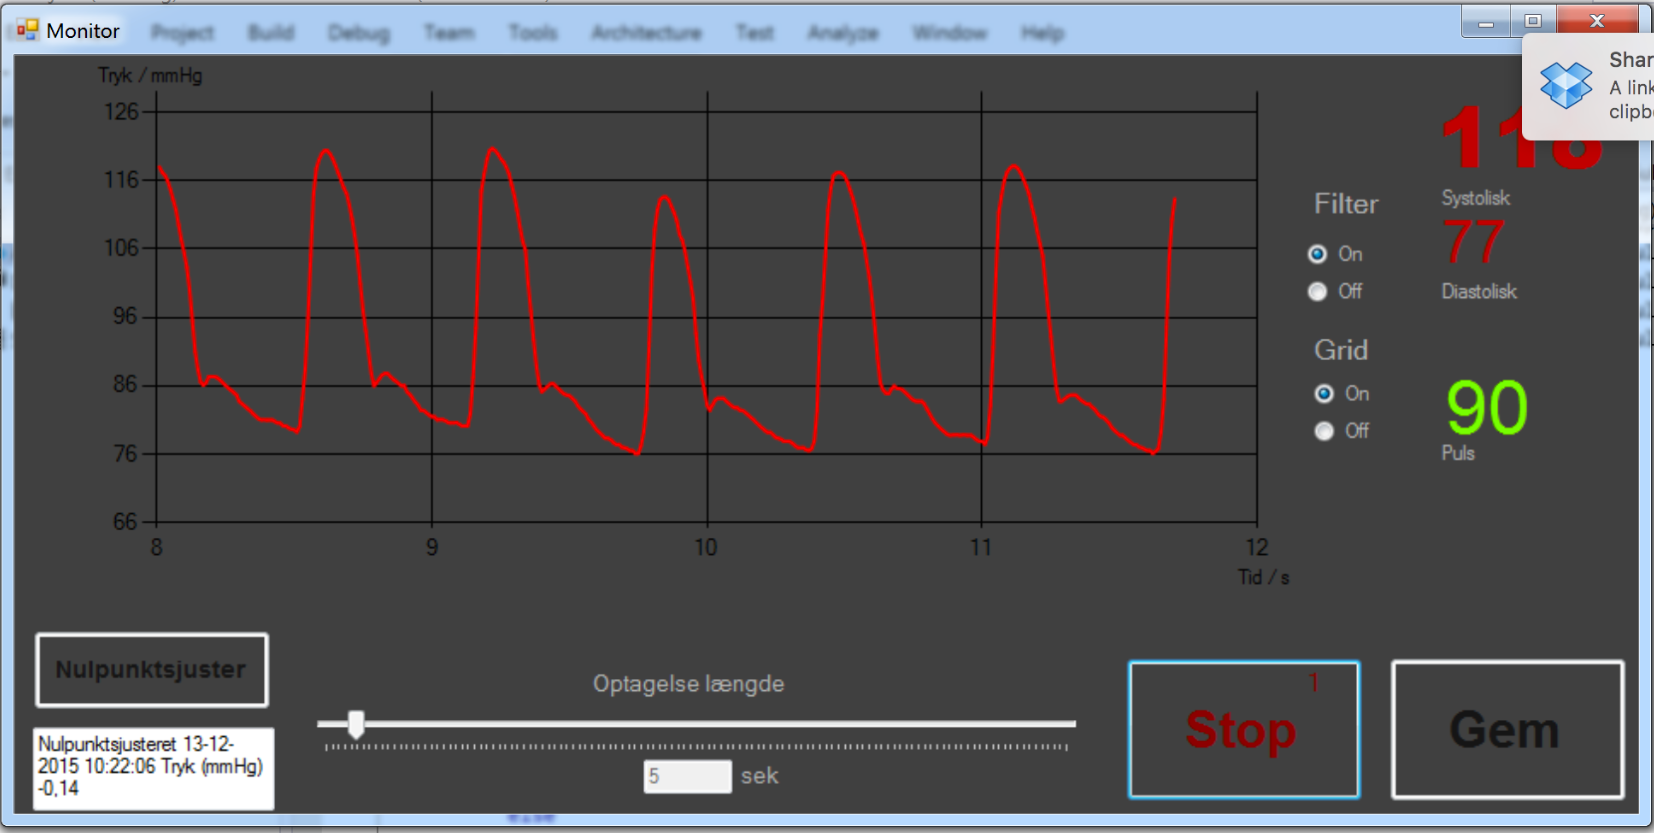
\includegraphics[width=1\textwidth]{Figurer/UC6_ForceRecEnd}
	\caption{Monitor-vindue efter tryk på "Rec"\--knap. "Rec"\--knappen skifter til en "Stop"\--knap}
\end{figure}

Metoden record() køres i Beregningerklassen. Her sættes startværdien for måling. Se Figur 4.39.

\begin{figure}[H]
	\centering
	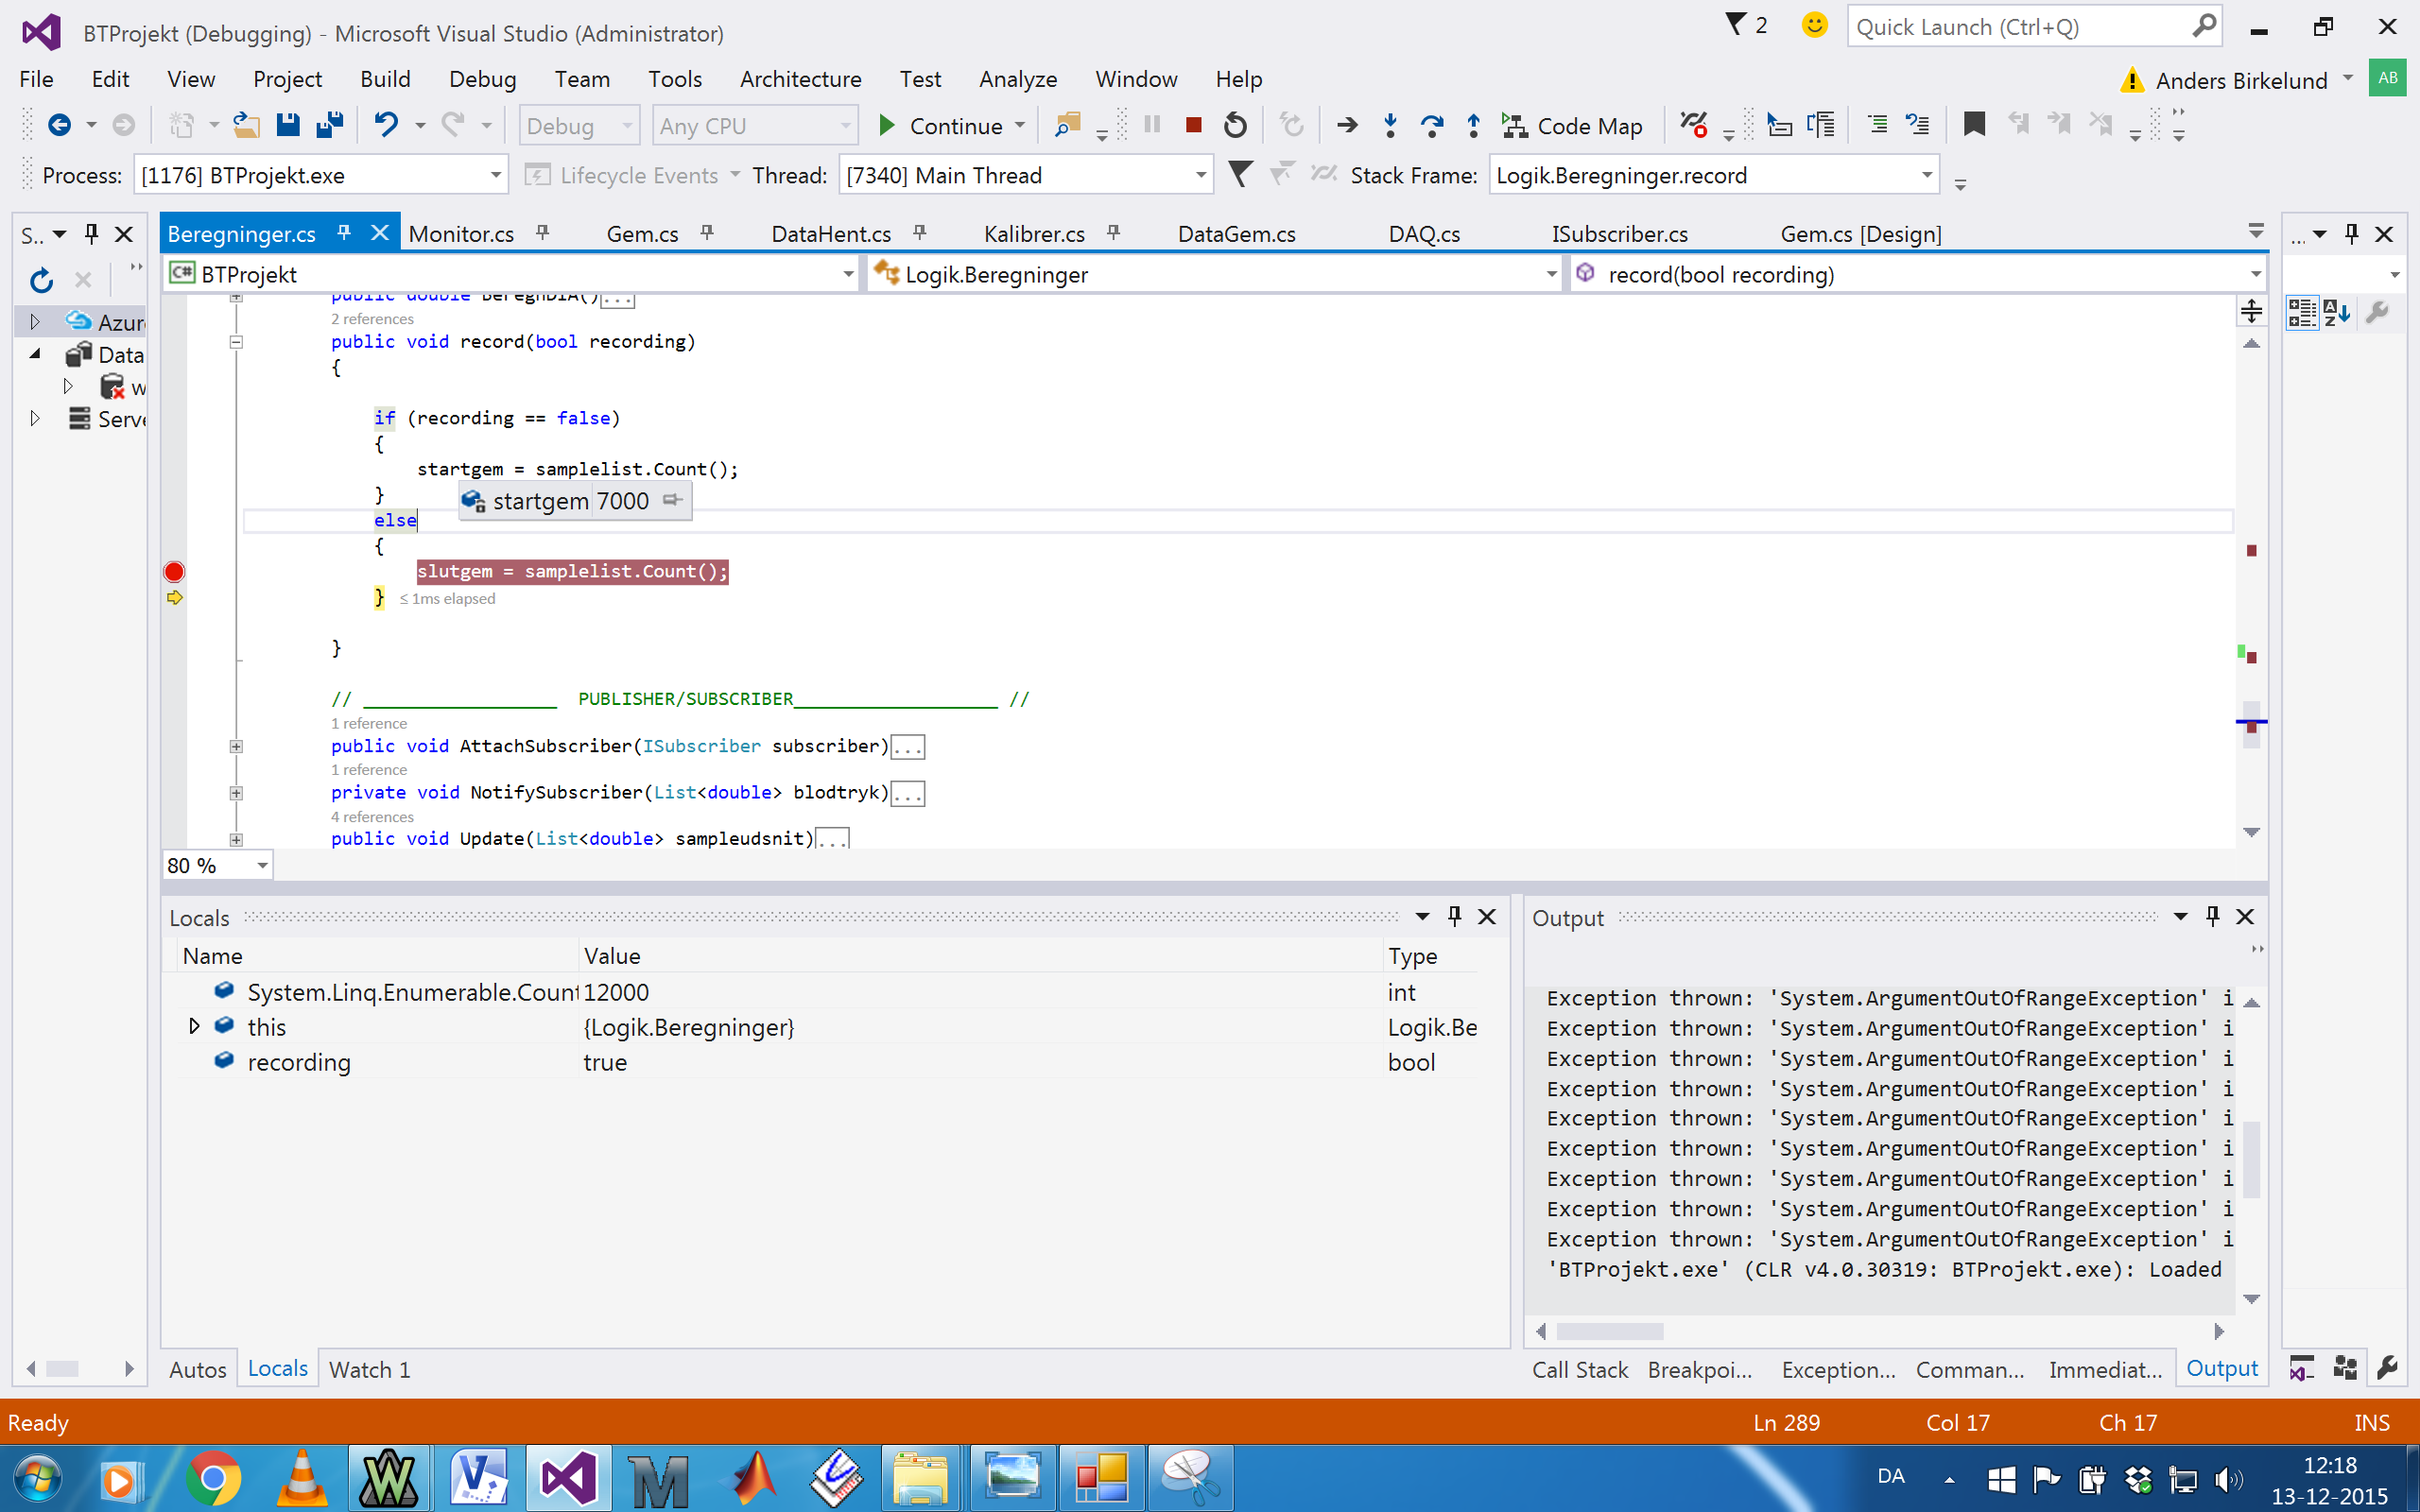
\includegraphics[width=1\textwidth]{Figurer/UC6_Record_Start}
	\caption{Beregningerklassens metode record() køres, når optagelse starter, og startværdien sættes}
\end{figure}

Tiden udløber og optagelsen slutter. Metoden record() køres automatisk igen. Denne gang sættes slutværdien for målingen. Det observeres om differencen mellem startværdi og slutværdi er lig 5 sekunder, det vil sige 5000 samples. Se Figur 4.40.

\begin{figure}[H]
	\centering
	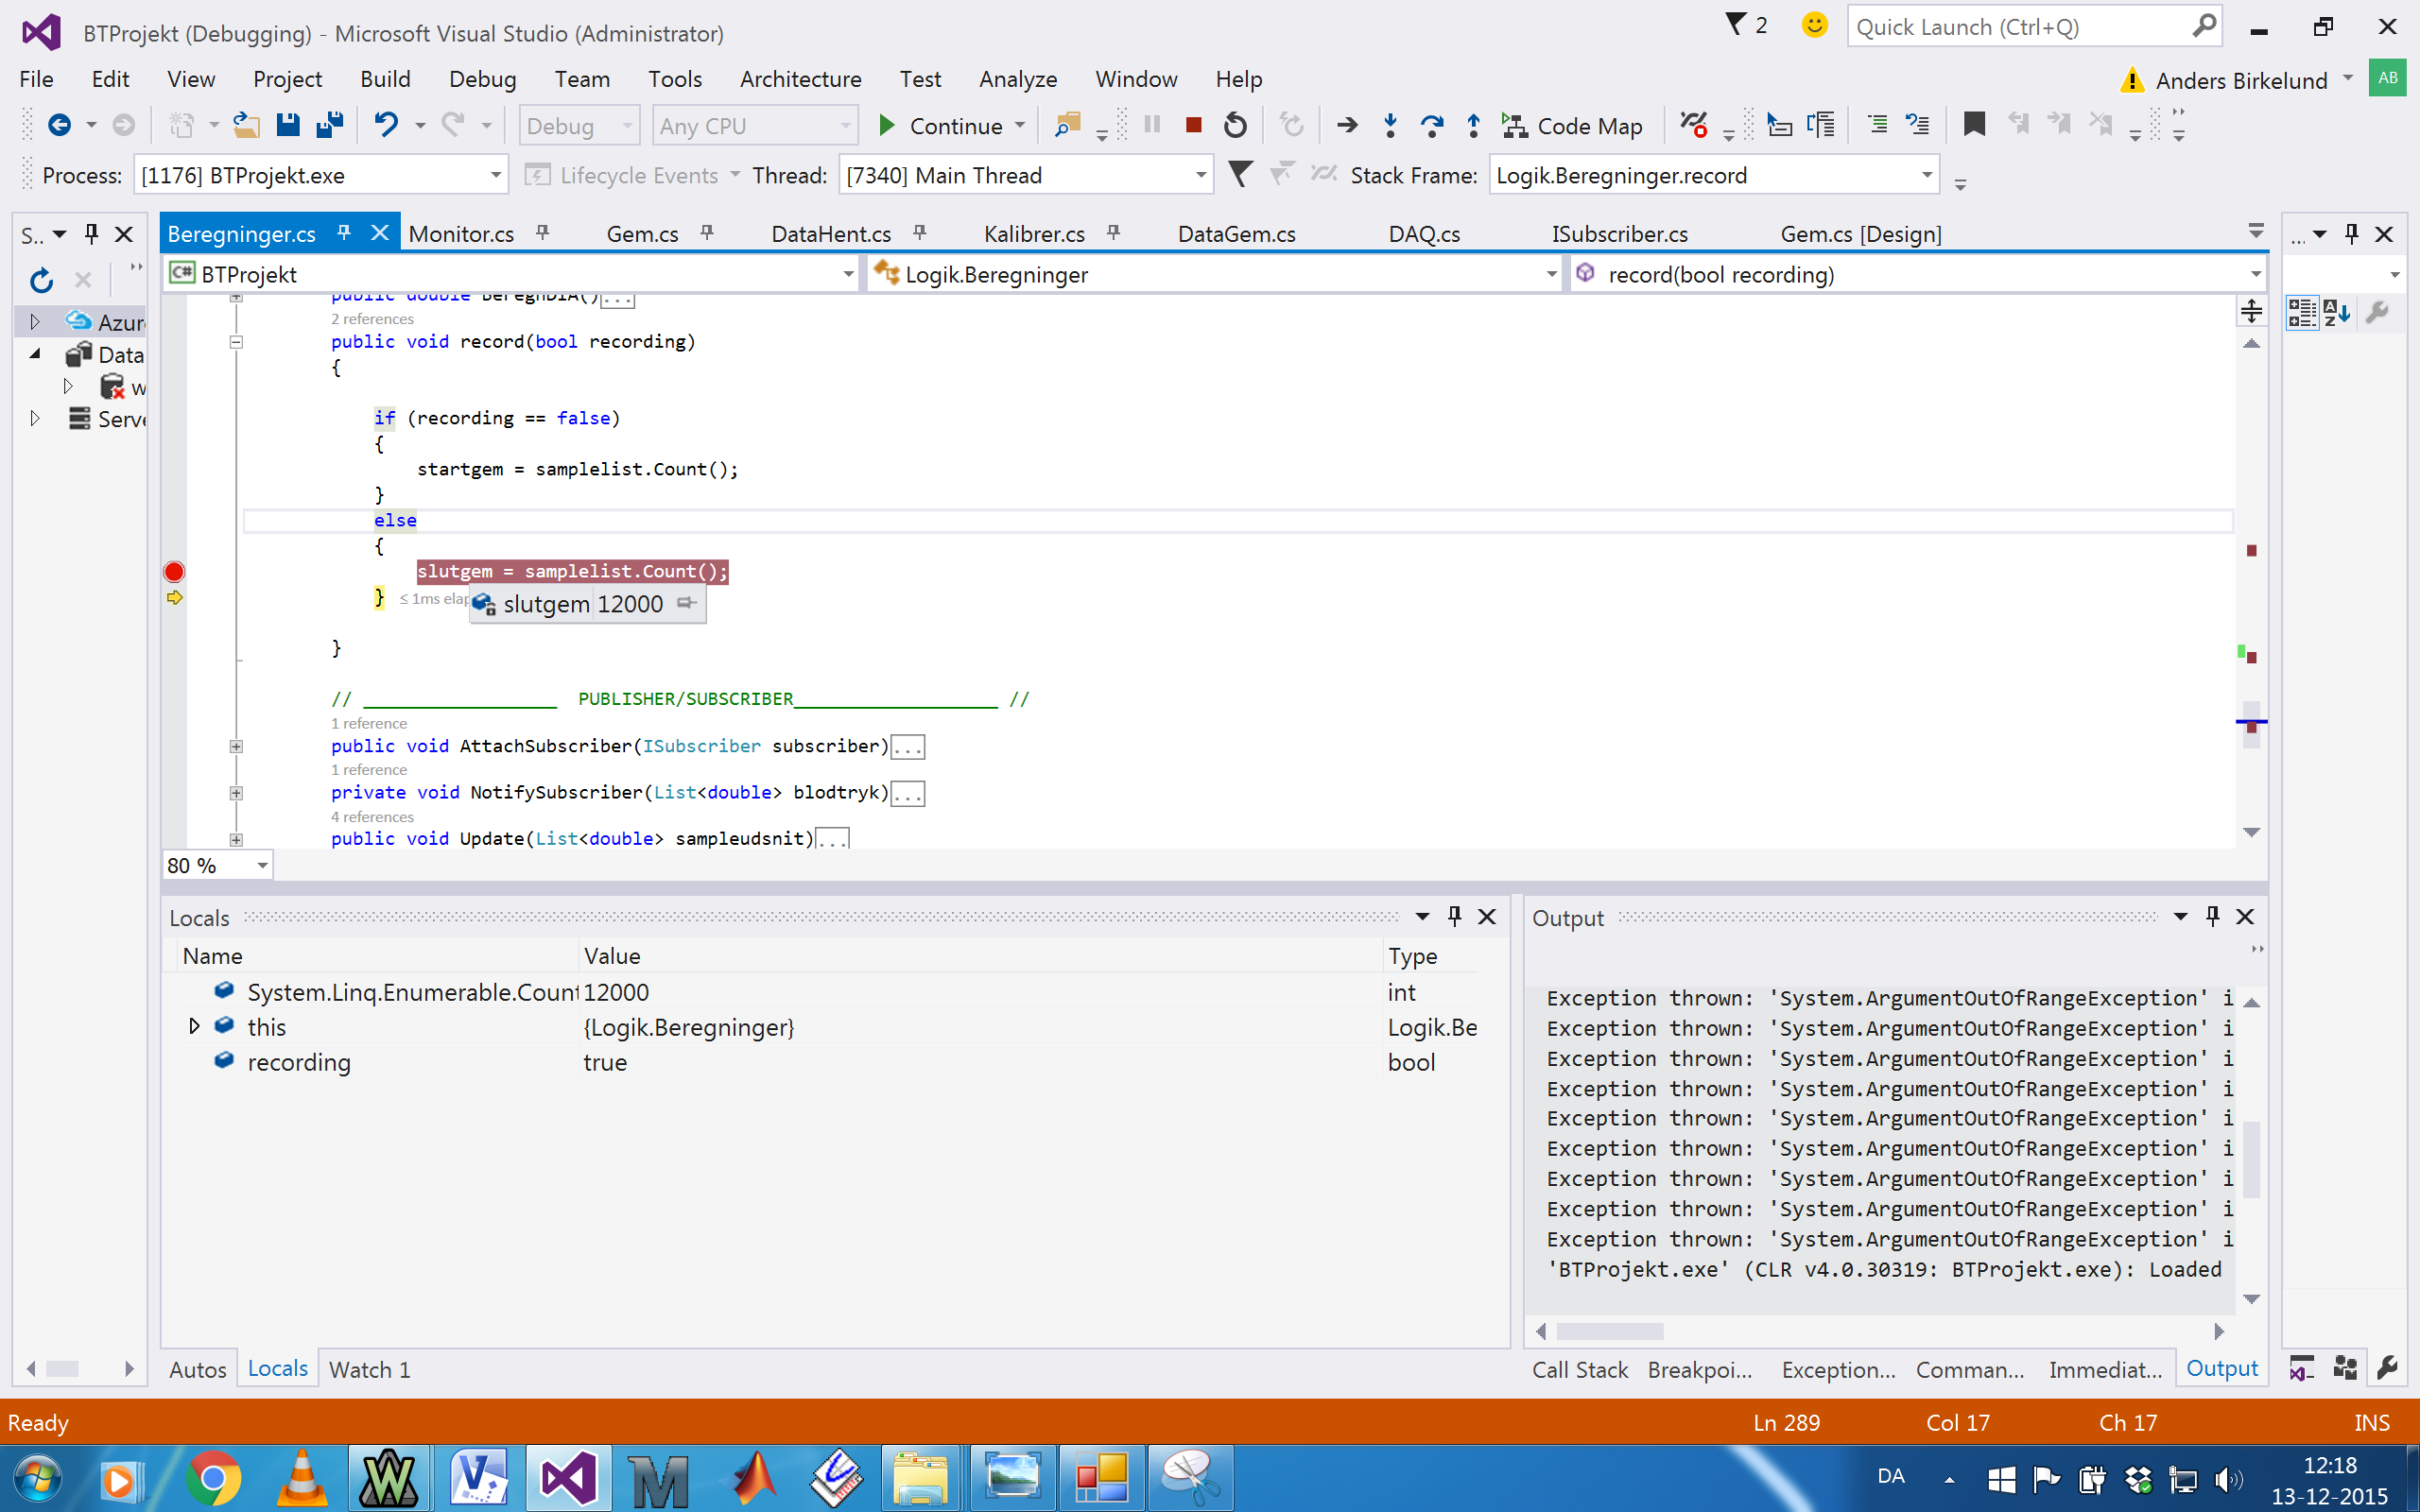
\includegraphics[width=1\textwidth]{Figurer/UC6_Record_Slut}
	\caption{Beregningerklassens record() køres når optagelse slutter, os slutværdien sættes}
\end{figure}

Forsker trykker på "Gem"\--knap i Monitor-vinduet. Gem-vinduets constructor modtager værdier via metoder, der afvikles i beregninger. Metoderne Visgemgraf() og Show() afvikles. Se Figur 4.41.

\begin{figure}[H]
	\centering
	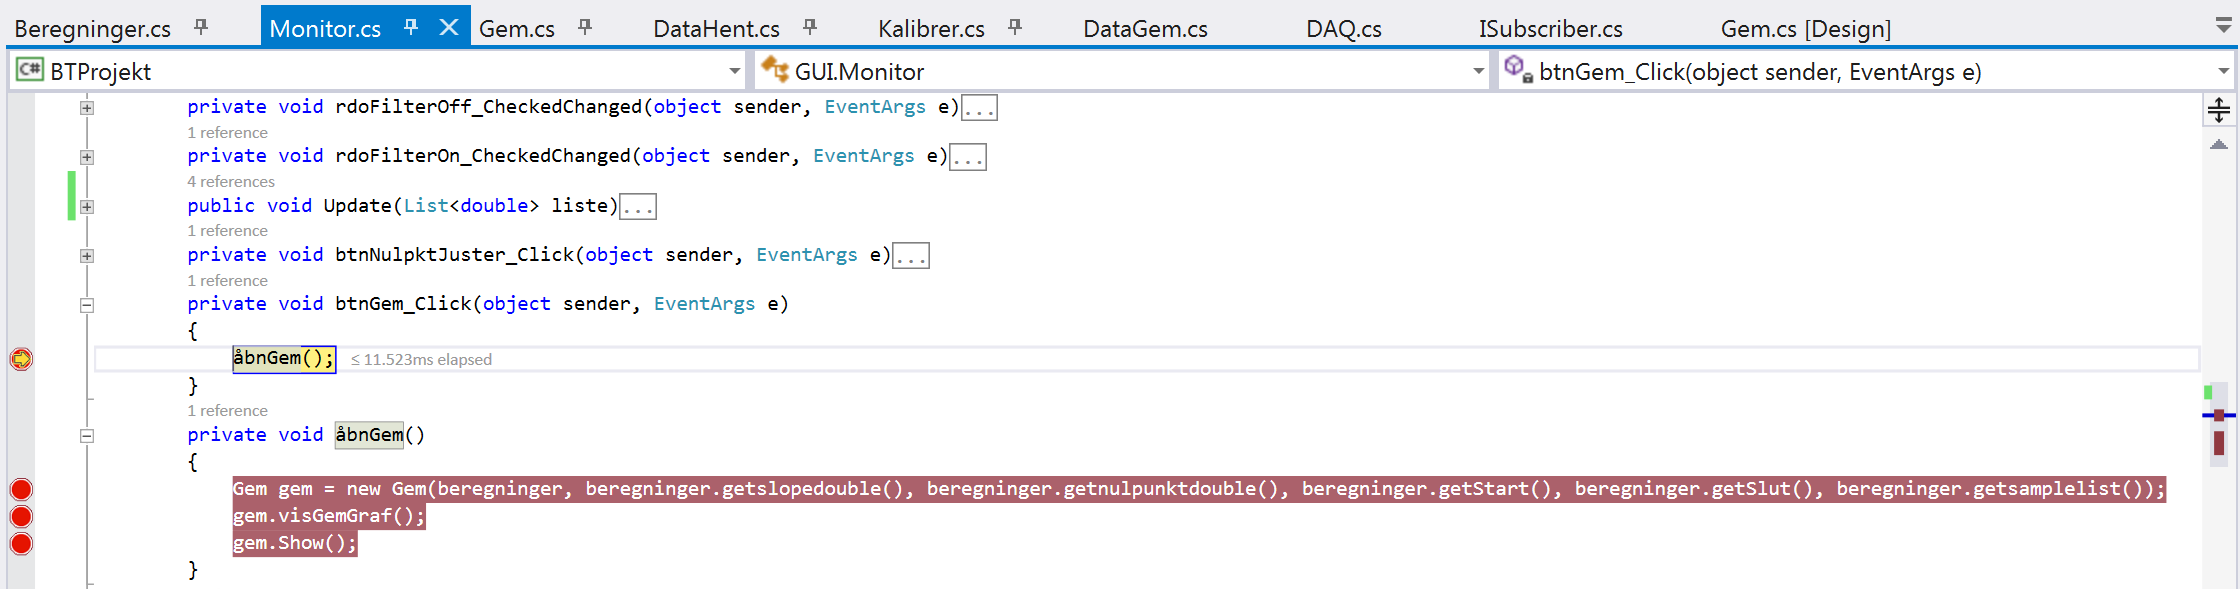
\includegraphics[width=1\textwidth]{Figurer/UC6_BtnGem}
	\caption{Oprettelse af nyt Gem-vindue}
\end{figure}

Det kontrolleres, om Gem-klassens værdier er korrekte. Følgende værdier tjekkes: slope\_ = kalibreringskonstant, nulpunkt\_ = nulpunktstryk, startgem\_ = startværdi for måling, slutgem\_ = slutværdi for måling. Se Figur 4.42.

\begin{figure}[H]
	\centering
	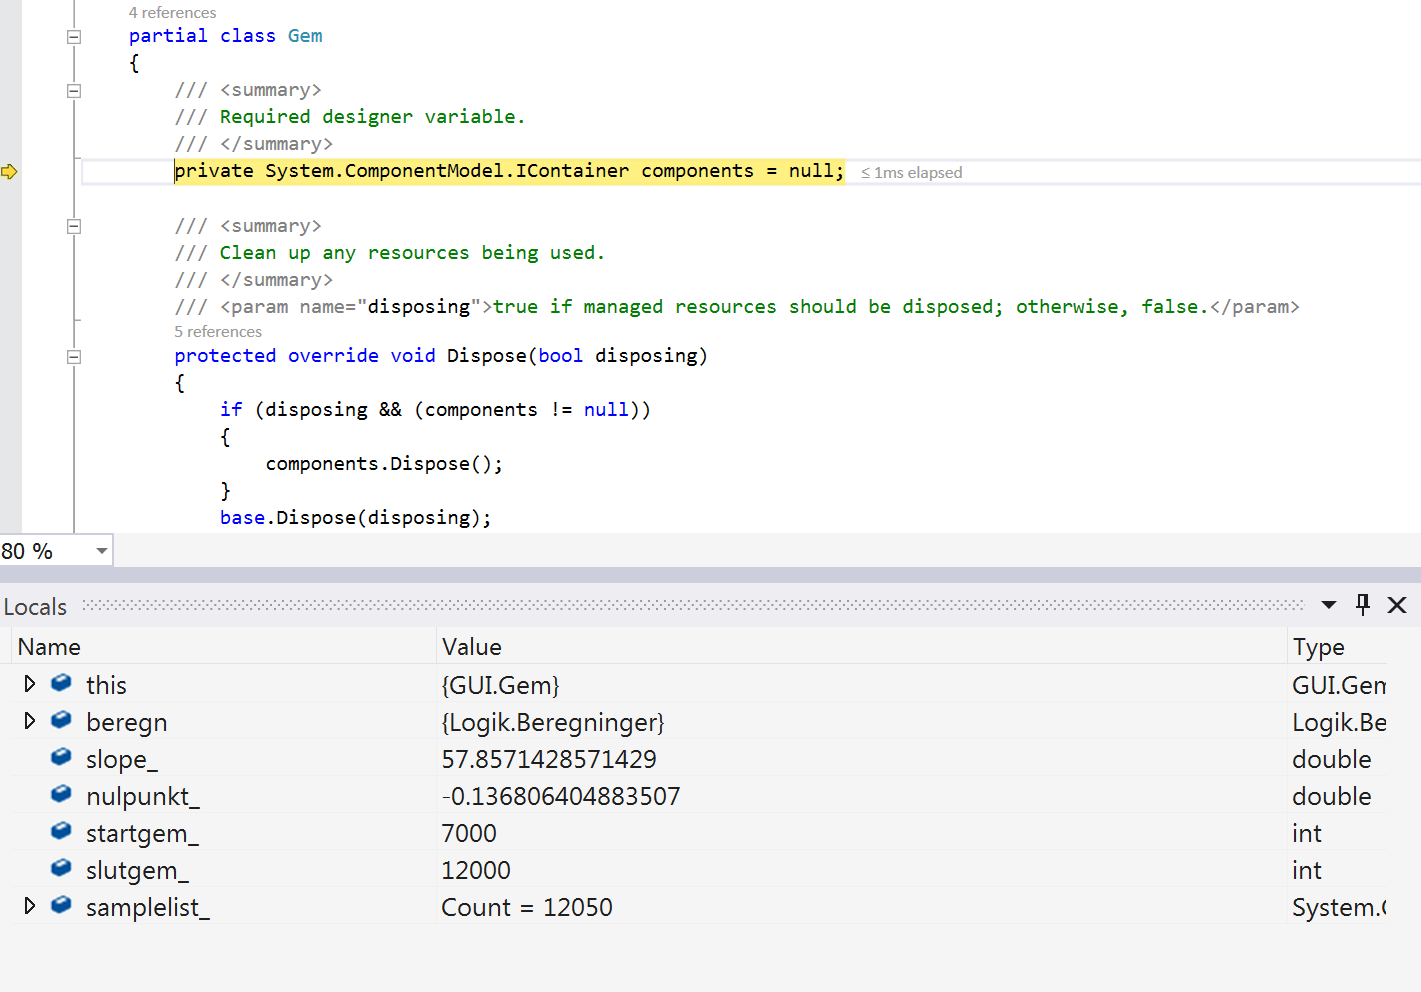
\includegraphics[width=1\textwidth]{Figurer/UC6_Vardier}
	\caption{Gem-vinduets værdier, efter oprettelse}
\end{figure}

Det kontrolleres, om længden af "samplearray" i metoden gemmaalingtilDB() stemmer overens med de valgte fem sekunder, det vil sige 5000 samples. Se Figur 4.43.

\begin{figure}[H]
	\centering
	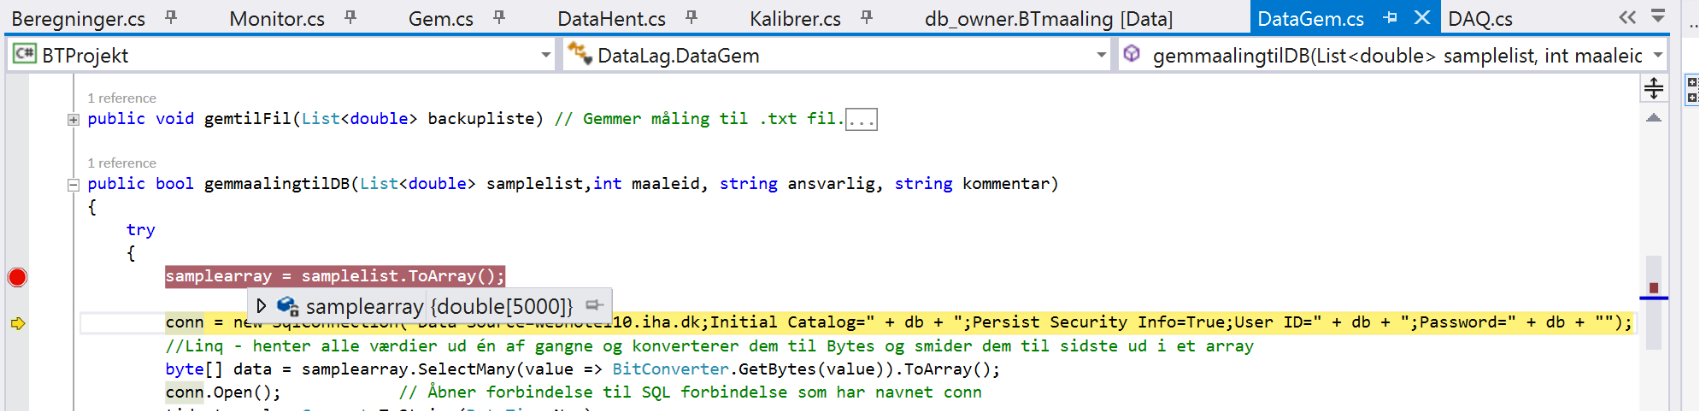
\includegraphics[width=1\textwidth]{Figurer/UC6_Samplearray}
	\caption{Array af blodtryksværdier, der gemmes til Database}
\end{figure}

Målingens ID noteres i Gem-vinduet. Se Figur 4.44.

\begin{figure}[H]
	\centering
	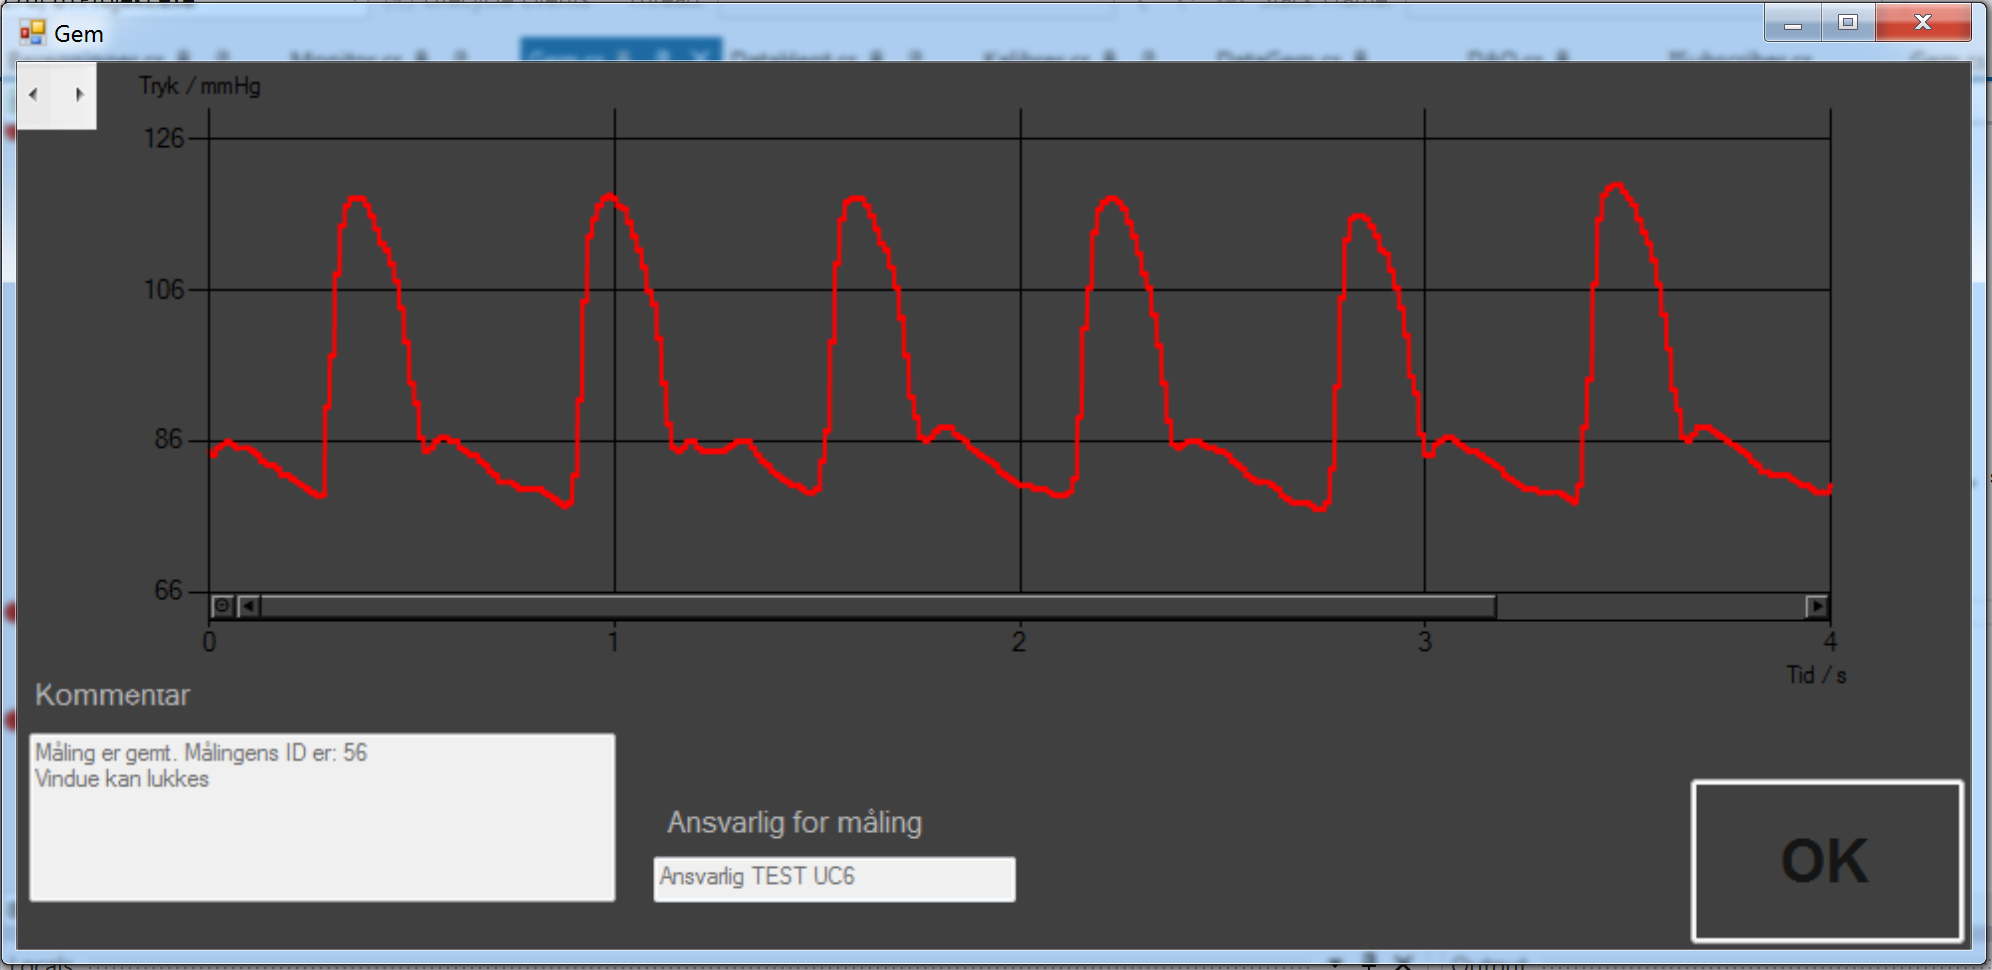
\includegraphics[width=1\textwidth]{Figurer/UC6_MalSuc}
	\caption{Gem-vinduet efter gemt måling}
\end{figure}


Det kontrolleres, om den gemte måling befinder sig i Databasen. Se Figur 4.45.

\begin{figure}[H]
	\centering
	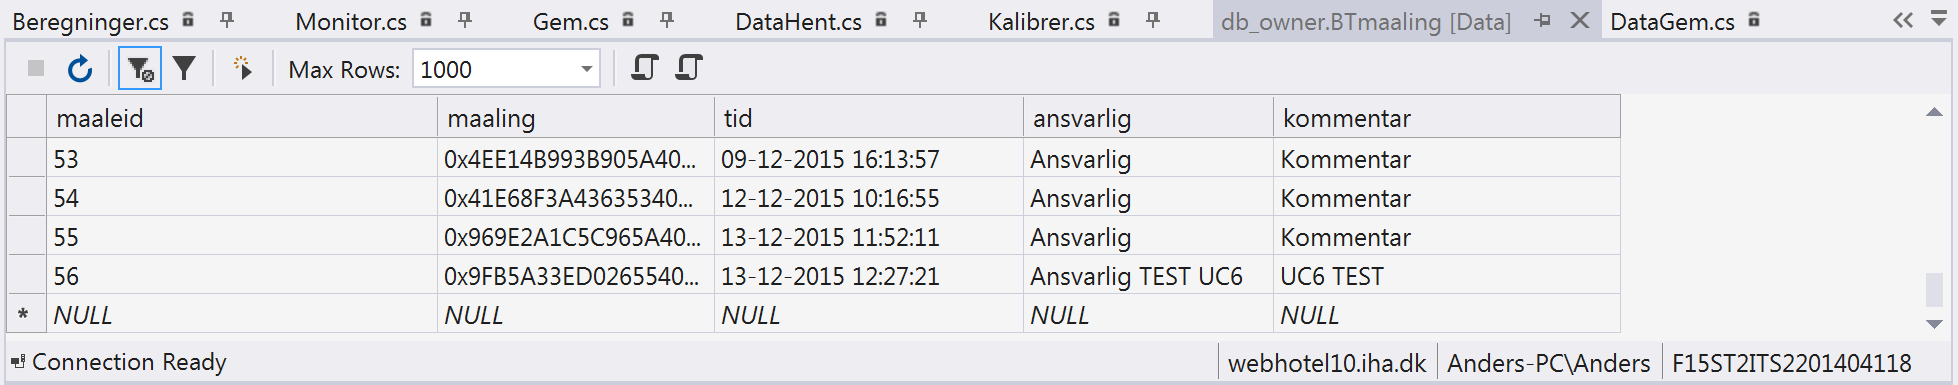
\includegraphics[width=1\textwidth]{Figurer/UC6_Database2}
	\caption{Array af blodtryksværdier, der gemmes til Database}
\end{figure}





